% !TEX root = catron-dissertation.tex
% arara: pdflatex
% arara: bibtex
% arara: pdflatex
% arara: pdflatex

\documentclass[twoadvisors,noinfo]{nddiss2e}

\usepackage{graphicx}
\usepackage{subcaption}
\usepackage{epstopdf}
\epstopdfsetup{outdir=./images/}
\usepackage{listings}
\usepackage{amsmath,amssymb}
% \usepackage[makeroom]{cancel}
% \usepackage{csquotes}
% \usepackage{fdsymbol}
% \usepackage{physics}
% \usepackage{mathtools}
\usepackage[export]{adjustbox}
\usepackage{multirow}
\usepackage{longtable,tabularx}
\usepackage{xcolor}
\usepackage{tikz}
\newcommand*\circled[1]{\tikz[baseline=(char.base)]{
    \node[shape=circle,draw,inner sep=2pt] (char) {#1};}}
\newcommand*\circledfill[1]{\tikz[baseline=(char.base)]{
    \node[shape=circle,draw,inner sep=2pt,fill=white] (char) {#1};}}
\newcommand*\squared[1]{\tikz[baseline=(char.base)]{
    \node[shape=rectangle,draw,inner sep=2pt] (char) {#1};}}

\lstset
{ %Formatting for code in appendix
    language=Matlab,
    basicstyle=\footnotesize,
    numbers=left,
    stepnumber=1,
    showstringspaces=false,
    tabsize=1,
    breaklines=true,
    breakatwhitespace=false,
}

% Custom Math Objects
\DeclareMathOperator{\fft}{FFT}
\DeclareMathOperator{\fftn}{FFT_n}
\DeclareMathOperator{\fftthree}{FFT_3}
\DeclareMathOperator{\ffttwo}{FFT_2}
\DeclareMathOperator{\fftshift}{FFT_{SHIFT}}
\DeclareMathOperator{\ifft}{IFFT}
\DeclareMathOperator{\ifftn}{IFFT_n}
\DeclareMathOperator{\wf}{WF}
\DeclareMathOperator{\f}{F}
\DeclareMathOperator{\opd}{OPD}
\DeclareMathOperator{\opdrms}{OPD_{RMS}}
\DeclareMathOperator{\opl}{OPL}
\DeclareMathOperator{\sr}{SR}
\DeclareMathOperator{\spl}{SPL}
\DeclareMathOperator{\real}{REAL}
\DeclareMathOperator{\imag}{IMAG}
\DeclareMathOperator{\ft}{FT}


\begin{document}
  \frontmatter
    \title{ Filtering of Acoustic Information from Aero-Optical Measurements }
    \author{ Brian Lowell Catron }
    \work{ Dissertation }
    \degaward{ Doctor of Philosophy }
    \advisor{ R. Mark Rennie }
    \secondadvisor{ Eric J. Jumper}
    \department{ Aerospace and Mechanical Engineering}

    \maketitle
    \copyrightyear{ 2022 }
    \makecopyright

    \begin{abstract}
      % !TEX root = catron-dissertation.tex

With development of new airborne optical systems, there is a significant amount of effort being put into ensuring that the systems will meet the specified performance criteria.
A large portion of this effort is being put into maximizing the farfield performance of the optical system.
To meet this goal, the optical path difference variance over the aperture, a measure of the nearfield optical distortions, is being reduced as much as possible.
Part of this development process involves testing models of these systems with various configurations in wind tunnels.
In these tests, the optical disturbances due to the testing environment are becoming a large percentage of the measured optical disturbances.

It is now a necessity to be able to identify, measure, and remove the various noise sources that appear in aero-optical measurements that take place in wind tunnels.
One of the primary sources of signal noise in these measurements, is acoustics.
Both the wing-tunnel fan and the flow through out the tunnel generate large amounts of acoustic noise that travel throughout the tunnel as acoustic duct modes.
The fan primary generates strong narrow-band signals at the blade-passing frequency and its harmonics.
There is also a significant broad-band acoustic duct mode signals along with vibration related signals and strong mostly-steady optical lensing signals that add to the overall measurement.

The signal identification and filtering mostly take place in the multidimensional spectrum, where the optical wavefront is not only split into its temporal frequency components but also its spatial frequency components.
A significant portion of this dissertation is dedicated to analyzing optical wavefront in the multidimensional spectral space.
The combination of three filters is able to remove most of the noise signals while retaining most of the aero-optical signal.
A velocity filter, which retains a narrow band of signal that is traveling within a small velocity range, is able to remove most of the broad-band signal noise, especially at higher temporal-frequencies.
A forward filter, which retains on the portion of a signal that is traveling in the direction of flow, removes signal that the velocity filter is not able to at lower temporal-frequencies.
Finally a baseline filter, which identifies the baseline spectrum and removes narrow-band peaks.

    \end{abstract}
    \begin{dedication}
      To my wife Karen \& our son Arthur
    \end{dedication}

    \tableofcontents
    \listoffigures
    \listoftables
    \begin{symbols}[cl]
% A
\sym{Ap}{Aperture size - Typically diameter}
% B
% C
% D
% E
% F
% G
% H
% I
\sym{I}{Actual on target intensity}
\sym{I_0}{Diffraction-limited intensity}
% J
% K
\sym{k}{Wavenumber ($k=2\pi/\lambda$)}
% L
% M
% N
\sym{n}{Index of refraction}
% O
\sym{\opd}{Optical path difference}
\sym{\opdrms}{Time-averaged spatial $\opd$ root-mean-square}
\sym{\opdrms(t)}{Spatial $\opd$ root-mean-square as a function of time}
% P
% Q
% R
% S
\sym{\sr}{Strehl ratio ($\textrm{SR}=I/I_0$)}
% T
% U
% V
% W
% X
% Y
% Z
\sym{}{\textbf{Greek}}
% ALPHA
% BETA
% GAMMA
% DELTA
\sym{\delta}{Boundary layer thickness}
% EPSILON
% ZETA
% ETA
% THETA
\sym{\left<\theta^2\right>}{Mean-squared of the fluctuating deflection angle}
% IOTA
% KAPPA
% LAMBDA
% MU
% NU
% XI
% OMICRON
% PI
% RHO
% SIGMA
% TAU
% UPSILON
% PHI
% CHI
% PSI
% OMEGA
\end{symbols}


    \begin{acknowledge}
      I would like to thank my advisors R. Mark Rennie and Eric J. Jumper along with Stanislav Gordeyev for helping me grow not only in my ability to take measurements, but also as a researcher, designing experiments and analyzing the data.

    \end{acknowledge}

  \mainmatter
    % !TEX root = catron-dissertation.tex
\epstopdfsetup{outdir=./images/01_introduction/}

\chapter{Introduction}
\label{chap:01_intro}

Directed-energy systems have a variety of uses but typically fall into one of two categories: communications and weapons.
The primary benefits of directed-energy communications is the ability to have secure point-to-point data transfer that is high unlikely to intercept or be interfered with \cite{crs-2021-RwNjGeZD}.
Directed-energy weapons are likely to have a lower cost per shot and a deeper magazine when compared to traditional munitions \cite{crs-2021-hyCUE868}.
As ground based directed-energy systems are slowly rolled out, most prominently aboard the USS Ponce \cite{crs-2021-Atxb7GDv}, there is a desire to field a system aboard an aircraft.

There have been two major attempts to field a directed-energy system aboard an aircraft to date \cite{Jumper-2013-8KtN3pue}.
The first was the Airborne Laser Laboratory (ALL) which took place in the late 1970's and early 1980's which used a CO$_2$ laser at 10.6-$\mu$m.
The second was the Airborne Laser (ABL) program which operated in the 2000's and used a COIL laser at 1.315-$\mu$m.
Airborne optical systems have to deal with a phenomenon know as ``aero-optics,'' which is optical distortions caused by various aero-dynamic flow features.
These optical distortions were first noticed due to image degradation in wind tunnel measurements in the 1950's \cite{Stine-1956-UaRzVZCe} as well as in photo-reconnaissance missions in the 1960's \cite{Kyrazis-2013-vwKeEBym}.

The intensity of that makes through an optical disturbance to a target, $I$, divided by the diffraction-limited performance, $I_0$, is known as the Strehl ratio \cite{Mahajan-1982-kkXM4eaB}, $\sr$,
\begin{equation}
  \sr = \frac{I}{I_0} \textrm{.}
  \label{eqn:01_strehl_ratio_definition}
\end{equation}
The diffraction-limited performance is the intensity that would make it to the same target if not for a disturbance.
The Airborne Laser Laboratory had an estimated Strehl ratio of 95\%\cite{Jumper-2013-8KtN3pue} meaning the ``aero-optics problem'' effectively did not apply.
After the Airborne Laser Laboratory program there was a desire to move toward shorter wavelengths in order to take advantage of improved diffraction-limited performance \cite{Jumper-2001-6QDh7zDy},
\begin{equation}
  \frac{I_0}{P} = \frac{1}{\pi}\left(\frac{Ap}{\lambda z}\right)^2 \textrm{,}
  \label{eqn:01_farfield_intensity}
\end{equation}
where $P$ is the laser output power, $Ap$ is the aperture size, and $z$ is the propagation distance.
This improved diffraction-limited performance is shown in Figure \ref{fig:01_farfield_intensity}.
\begin{figure}
  \centering
  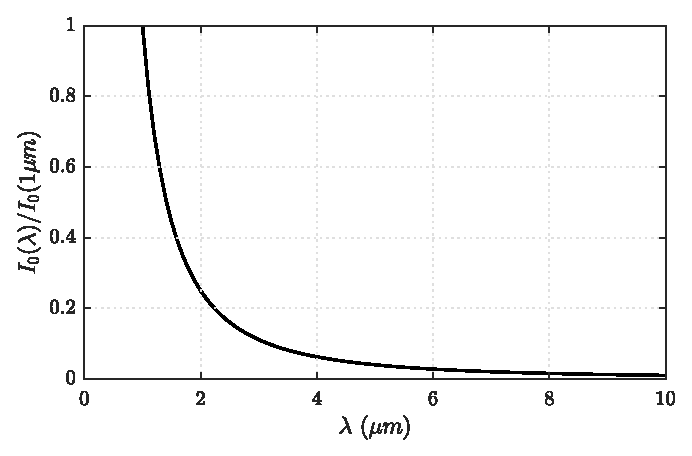
\includegraphics{../matlab/01_introduction/farfield_intensity.eps}
  \caption{Diffraction-limited far-field intensity of a beam normalized by the performance at 1-$\mu$m.}
  \label{fig:01_farfield_intensity}
\end{figure}
By only changing the laser source from a 10-$\mu$m to 1-$\mu$m wavelength the diffraction-limited performance can be increased 100 times.

Aero-optical issues start to become apparent as the wavelength is decreased as is evident by the Mar\'echal approximation \cite{Mahajan-1983-hg7ahvJM} which relates the Strehl ratio to wavelength,
\begin{equation}
  \sr \approx \exp\left\{-\left[\frac{2\pi \opdrms}{\lambda}\right]^2\right\} \textrm{,}
  \label{eqn:01_strehl_ratio}
\end{equation}
where $\opdrms$ is the spatial root-mean-square of the optical path difference over the aperture and is a way to quantify the optical disturbance that will be discussed in Chapter \ref{chap:02_lit_review}.
If the ALL system's laser was swapped with another laser of a lower wavelength, the Strehl ratio would significantly decrease as shown by Figure \ref{fig:01_strehl_ratio}.
\begin{figure}
  \centering
  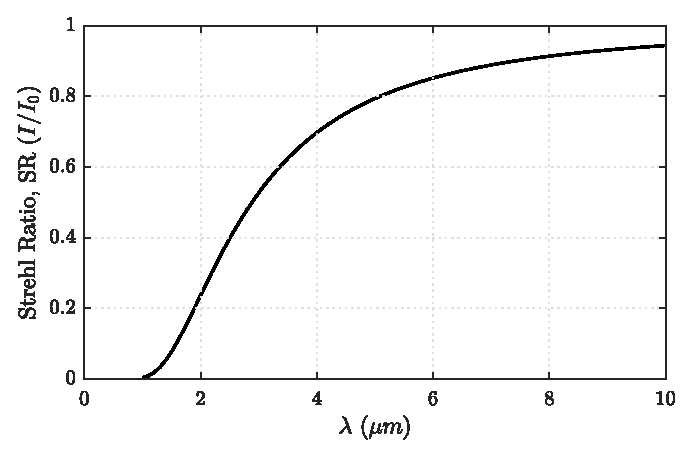
\includegraphics{../matlab/01_introduction/strehl_ratio.eps}
  \caption{Strehl ratio due to the $\opdrms$ of the Airborne Laser Laboratory (ALL) at various laser wavelengths.  ALL had an estimated Strehl ratio of 95\% with its 10.6-$\mu$m laser.}
  \label{fig:01_strehl_ratio}
\end{figure}
While the hypothetical case of going from 10 to 1-$\mu$m resulted in a 100-fold increase in diffraction-limited performance, the actual on-target intensity that this hypothetical system obtains would be essentially zero.
This means that the aero-optical problem can no longer be ignored and was recognized as one of the main developmental risks of the ABL program \cite{DOTE-1999-HnkadUEw}.
{\color{red}{Do you have or know of a source that at the very least alludes to the aero-optical issues with ABL that greatly limited its field of regard?}}

As the next generation of airborne directed-energy systems are developed some amount of ground testing of those systems will need to occur.
In order to understand the aero-optical environment that these systems will experience in the air wind tunnel tests will need to be employed.
These tests are far cheaper to perform and allow for quicker iteration of design parameters.
Wind tunnel tests will however include some additional optical contamination including but not limited to the boundary layer present on the wall and the acoustic environment generated by the wind tunnel fan \cite{Gordeyev-2014-jcJndkHM}.
Assuming that the optical disturbances system model are statistically independent from the optical disturbances from the testing environment, we can estimate the total optical disturbance from
\begin{equation}
  \opdrms_{TOTAL}^2 = \opdrms_{MODEL}^2+\opdrms_{ENVIRONMENT}^2 \textrm{.}
  \label{eqn:01_combined_opd}
\end{equation}

This combination of optical disturbances is shown in Figure \ref{fig:01_design_iteration} along with a hypothetical iterative design process.
\begin{figure}
  \centering
  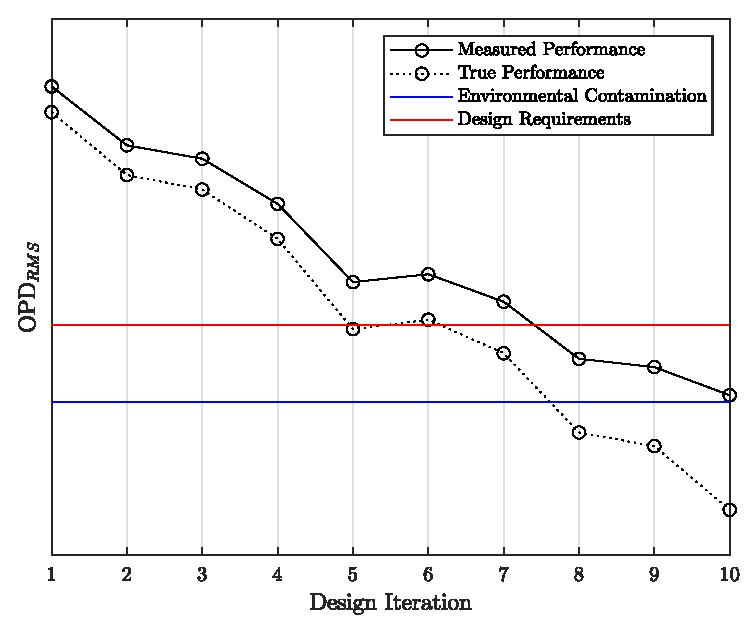
\includegraphics{../matlab/01_introduction/design_iteration.eps}
  \caption{Hypothetical iterative design process of an airborne directed-energy system.  The required performance level is shown by the red line and the testing environment's contamination is shown by the blue line.}
  \label{fig:01_design_iteration}
\end{figure}
This process seeks to obtain a design that meets a required level of performance shown in red.
If only the measured data is used to assess the system's performance three additional iterative changes are needed to achieve a usable design which can add significantly to the development time and costs.
If the environmental contamination is greater than the design requirement, the measured performance will never reach the required performance criteria.
When the true performance of a system is significantly higher than the environmental contamination, the measured performance is not significantly greater than the true performance.
The measured performance becomes significantly greater that the true performance when the true performance is less than the environmental contamination.

This dissertation will primary examine the environmental contamination due to acoustic noise within the wind tunnel.
In Chapter \ref{chap:03_optical_acoustics} it will look at the optical disturbances caused by acoustic waves from some simple plane and spherical waves to a process for estimating the acoustic environment within the test section of a wind tunnel.
The strength of an spherical acoustic wave will be assessed with both microphone and optical measurements.
Multi-dimensional spectral techniques will be used to analyze optical wavefronts in Chapter \ref{chap:04_dispersion} and filter optical wavefronts in Chapter \ref{chap:06_single_filter}.
These filtering techniques will contain some optical contamination particularly in regions where the various signal components interfere with one another.
In order to further reduce the optical contamination, Chapter \ref{chap:07_multiple_filter} will utilize additional sensor information from both microphones and accelerators to remove some of the overlapping contamination to obtain a better picture of the actual optical performance of an airborne directed-energy system from ground test measurements.

    % !TEX root = catron-dissertation.tex
\epstopdfsetup{outdir=./images/02_background/}

\chapter{Literature Review}
\label{chap:02_lit_review}
The literature review will consist of primarily two sections.
The first section will examine aero-optics while the second will look at acoustics inside of ducts.
\section{Aero-Optics}
Optical communication and directed energy systems require a tightly focused beam on target in order to meet system performance objectives.
The farfield performance of airborne optical systems can be degraded by the nearfield flow that becomes optically active at compressible flow speeds.
``Aero-optics'' is the study of the optical effect of these nearfield flow disturbances.
Examples of important aero-optical flows that have been studied extensively include boundary layers \cite{Gordeyev-2014-jcJndkHM,Smith-2013-VXArwwux,Wang-2012-gJ7rttg7}, shear layers \cite{Fitzgerald-2004-DgAgbreK,Rennie-2008-Wku6NheG}, shock waves \cite{Jumper-2013-8KtN3pue}, and even tip vortices \cite{Porter-2013-pQcNWHJ6}.
The effect of acoustic disturbances on aero-optical measurements has also been shown in both flight testing \cite{DeLucca-2018-gBQdjTmT} and ground testing \cite{Catron-2018-DdVp6VZf,Catron-2020-x8njYmmu}.

In these optically active flows the index-of-refraction, $n$, varies locally as does the other fluid properties.
Gladstone and Dale \cite{Gladstone-1863-ND4wtDT9} found that the index-of-refraction is primarily a function of density with a loose dependence on the wavelength of light.
Gladstone and Dale proposed a ``specific refractive energy'' now known as the Gladstone-Dale constant, $K_{GD}$,
\begin{equation}
  K_{GD} = \frac{n-1}{\rho}\textrm{.}
  \label{eqn:02_gladstone_dale_constant}
\end{equation}
For air the refractive index can be related to state quantities \cite{Valley-1965-F3k3cmv6}
\begin{equation}
  n-1 = 77.6\times 10^{-6}\frac{P}{T}\left(1+\frac{7.53\times10^{-3}}{\lambda^2}\right)\textrm{,}
  \label{eqn:02_refractive_index_ptlambda}
\end{equation}
where $P$ is in mbar, $T$ is in K, and $\lambda$ is in $\mu$m.
By combining this relationship with the ideal gas law, the Gladstone-Dale constant can be determined as a function of light wavelength,
\begin{equation}
  K_{GD} = 2.23\times10^{-4}\left(1+\frac{7.53\times10^{-3}}{\lambda_{\mu m}^2}\right) \: \left[\frac{m^3}{kg}\right]\textrm{.}
  \label{eqn:02_gladstone_dale_wavelength}
\end{equation}
The Gladstone-Dale constant for air over the visible range is shown in Figure \ref{fig:02_gladstone_dale_wavelength}.
\begin{figure}
  \centering
  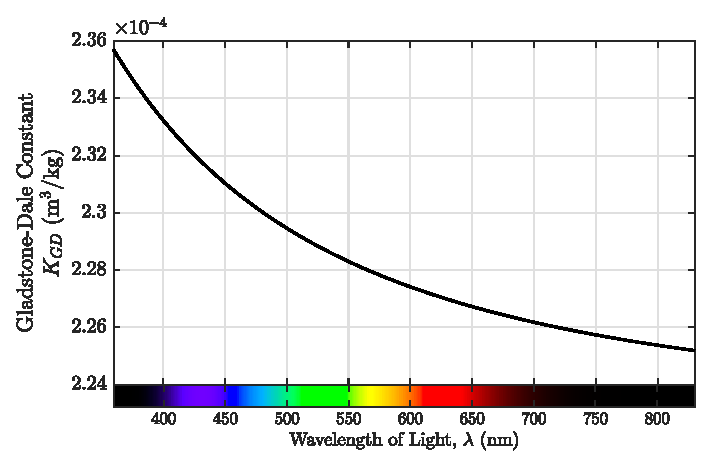
\includegraphics{../matlab/02_background/gladstone_dale_wavelength.eps}
  \caption{Gladstone-Dale constant for air over the visible wavelength range.}
  \label{fig:02_gladstone_dale_wavelength}
\end{figure}
While the value for $K_{GD}$ does vary over the visible range, it is only a few percent, and many sources use an average value of 2.27$\times10^{-4}$ m$^3$/kg for the visible and near-infrared \cite{Gardiner-1980-reW8xrCb}.
The Gladstone-Dale relationship is typically presented as
\begin{equation}
  n = 1+K_{GD}\rho
  \label{eqn:02_gladstone_dale_relation}
\end{equation}
but when applied to situations where there are significant fluctuations in the flow an alternate form is often more useful
\begin{equation}
  n'=K_{GD}\rho'
  \label{eqn:02_gladstone_dale_relation_fluctuating}
\end{equation}
where $'$ denotes the quantity represents the fluctuating component ($n' = n-\bar{n}$).

When a beam with an initially planar wave front passes through a region of optical active flow its wave front aberrated
The optical path length ($\opl$) at any point in the beam can be obtained by integrating the index of refraction along the propagation of an optical ray \cite{Klein-1986-8Vx29RfE}.
\begin{equation}
  \opl (x,y,t) = \int^{s_2}_{s_1} n(x,y,z,t)ds
  \label{eqn:02_opl}
\end{equation}
The optical path difference ($\opd$), is then the spatially-averaged $\textrm{OPL}$ over an aperture removed from the OPL.
\begin{equation}
  \opd(x,y,t) = \opl(x,y,t)-\langle\opl(x,y,t)\rangle
  \label{eqn:02_opd}
\end{equation}
When working with fluctuating components, the $\opd$ can be calculated directly
\begin{equation}
  \opd(x,y,t) = \int^{s_2}_{s_1} n'(x,y,z,t)ds \textrm{.}
  \label{eqn:02_opd_n}
\end{equation}

When $\opd$ is combined with the beam intensity profile, one can compute the farfield complex amplitude distribution using the Fraunhofer approximation \cite{Goodman-1968-zPUmuuzx}.
\begin{equation}
  U(x_0,y_0,t)\propto\iint_{Ap}\exp\left\{\frac{2\pi j}{\lambda}\left[\opd(x_1,y_1,t)-\frac{(x_0x_1+y_0y_1)}{z}\right]\right\}dx_1dy_1
  \label{eqn:02_fraunhofer}
\end{equation}
where $U$ is the complex amplitude, the subscripts 0 and 1 represent the coordinates of the farfield and nearfield respectively.
The intensity can be computed from the complex amplitude via: $I = UU^\ast$.
For cases in which optical aberrations are nonexistent (i.e. $\opd(x,y,t)=0$), the farfield irradiance pattern that results from Equation \ref{eqn:02_fraunhofer} is caused entirely by diffraction from the optical aperture, and is referred to as the “diffraction-limited” irradiance pattern.
For a beam with a flat wave front and circular aperture, the farfield irradiance pattern is the Airy’s disk, and the peak irradiance at the center of the disk, $I_0$ , is the maximum irradiance that can be achieved by the optical system:
\begin{equation}
  I_0 = \left(\frac{kAp^2}{8z}\right)^2
  \label{eqn:02_airy_pattern}
\end{equation}
where $k$ is the wavenumber ($k=2\pi /\lambda$), $Ap$ is the aperture diameter, and $z$ is the distance from the aperture.
In the presence of aero-optical aberrations, $\opd(x,y,t)$ is non-zero, and the farfield irradiance pattern in this case tends to be more spread out and diffuse than the diffraction-limited case; furthermore, the beam may be shifted off target by optical tip/tilt imposed by the aberrations.

The Strehl ratio ($\sr$), is the ratio of intensity on target ($I$) to the diffraction-limited on target intensity ($I_0$):
\begin{equation}
  \sr=\frac{I}{I_0}
  \label{eqn:02_strehl_simple}
\end{equation}
The Strehl ratio can be computed accurately by applying Equation \ref{eqn:02_fraunhofer} twice, once for the diffraction-limited case to obtain $I_0$, and a second time with the $\opd$ field due to aero-optical aberrations included to obtain $I$.
The farfield performance, can also be estimated via the Mar\'{e}chal approximation:
\begin{equation}
  \sr(t) \equiv \frac{I(t)}{I_0} \approx \exp \left\{-\left[\frac{2\pi \opdrms(t)}{\lambda}\right]^2\right\}
  \label{eqn:02_strehl_ratio}
\end{equation}
where $\opdrms$ is the spatial rms of the wave front and $\lambda$ is the wavelength of the beam.
\begin{figure}
  \centering
  \begin{subfigure}[t]{0.45\textwidth}
    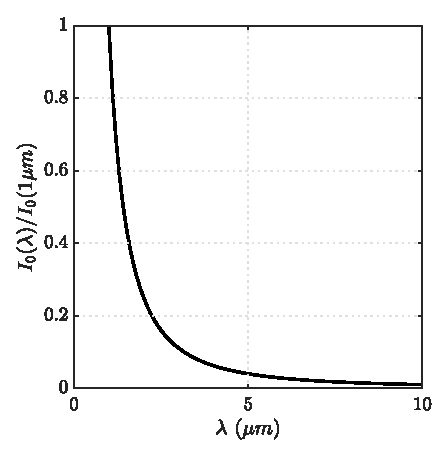
\includegraphics{../matlab/02_background/farfield_intensity.eps}
    \caption{}\label{fig:02_farfield_intensity}
  \end{subfigure}
  ~
  \begin{subfigure}[t]{0.45\textwidth}
    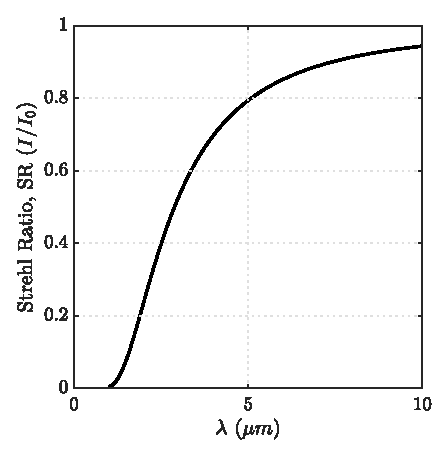
\includegraphics{../matlab/02_background/all_strehl_ratio.eps}
    \caption{}\label{fig:02_all_strehl_ratio}
  \end{subfigure}
  \caption{(\subref{fig:02_farfield_intensity}) Diffraction limited on target intensity as a function of wavelength normalized by the value at $\lambda$ = 1 $\mu$ m. (\subref{fig:02_all_strehl_ratio}) Strehl ratio as a function of wavelength for an aberration that gives SR = 0.95 at $\lambda$ = 10.6 $\mu$m.}
  % \label{FIG:airy_strehl}
\end{figure}
Equation \ref{eqn:02_strehl_ratio} shows a key relationship between $\opd$, wavelength, and the farfield performance, plotted in Figure \ref{fig:02_all_strehl_ratio}.
On the other hand, Equation \ref{eqn:02_airy_pattern} shows that the diffraction-limited farfield irradiance increases as the wavelength is shortened, plotted in Figure \ref{fig:02_farfield_intensity}.
Together, Figure \ref{fig:02_farfield_intensity} and \ref{fig:02_all_strehl_ratio} show that as modern optical systems move to shorter wavelengths to increase $I_0$, aero-optical aberrations cause a much more serious degradation of the Strehl ratio, illustrating why aero-optical considerations are critical in the development of any airborne optical system.

Figure \ref{fig:02_necessary_opd} shows the $\opdrms$ necessary to achieve various Strehl ratios over a range of wavelengths.
\begin{figure}
  \centering
  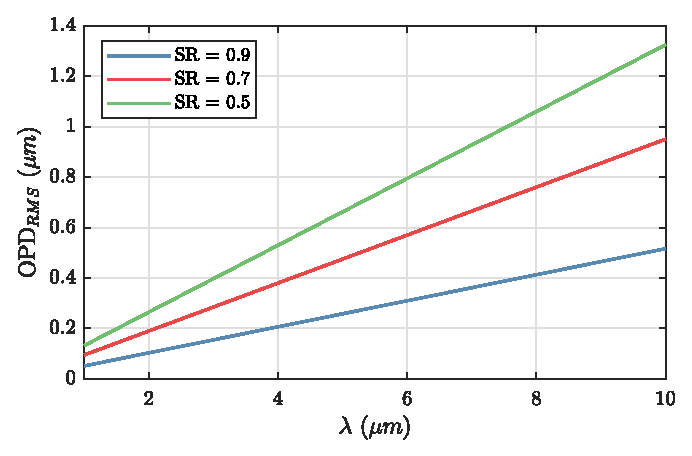
\includegraphics{../matlab/02_background/necessary_opd.eps}
  \caption{$\opdrms$ values necessary to obtain Strehl ratios of 0.9, 0.7, and 0.5 over a range of wavelengths.}
  \label{fig:02_necessary_opd}
\end{figure}
As the wavelength of light decreases the required $\opdrms$ decreases linearly for a fixed Strehl ratio.


\subsection{Typical Optical Wavefront Measurement System}





\begin{figure}
  \centering
  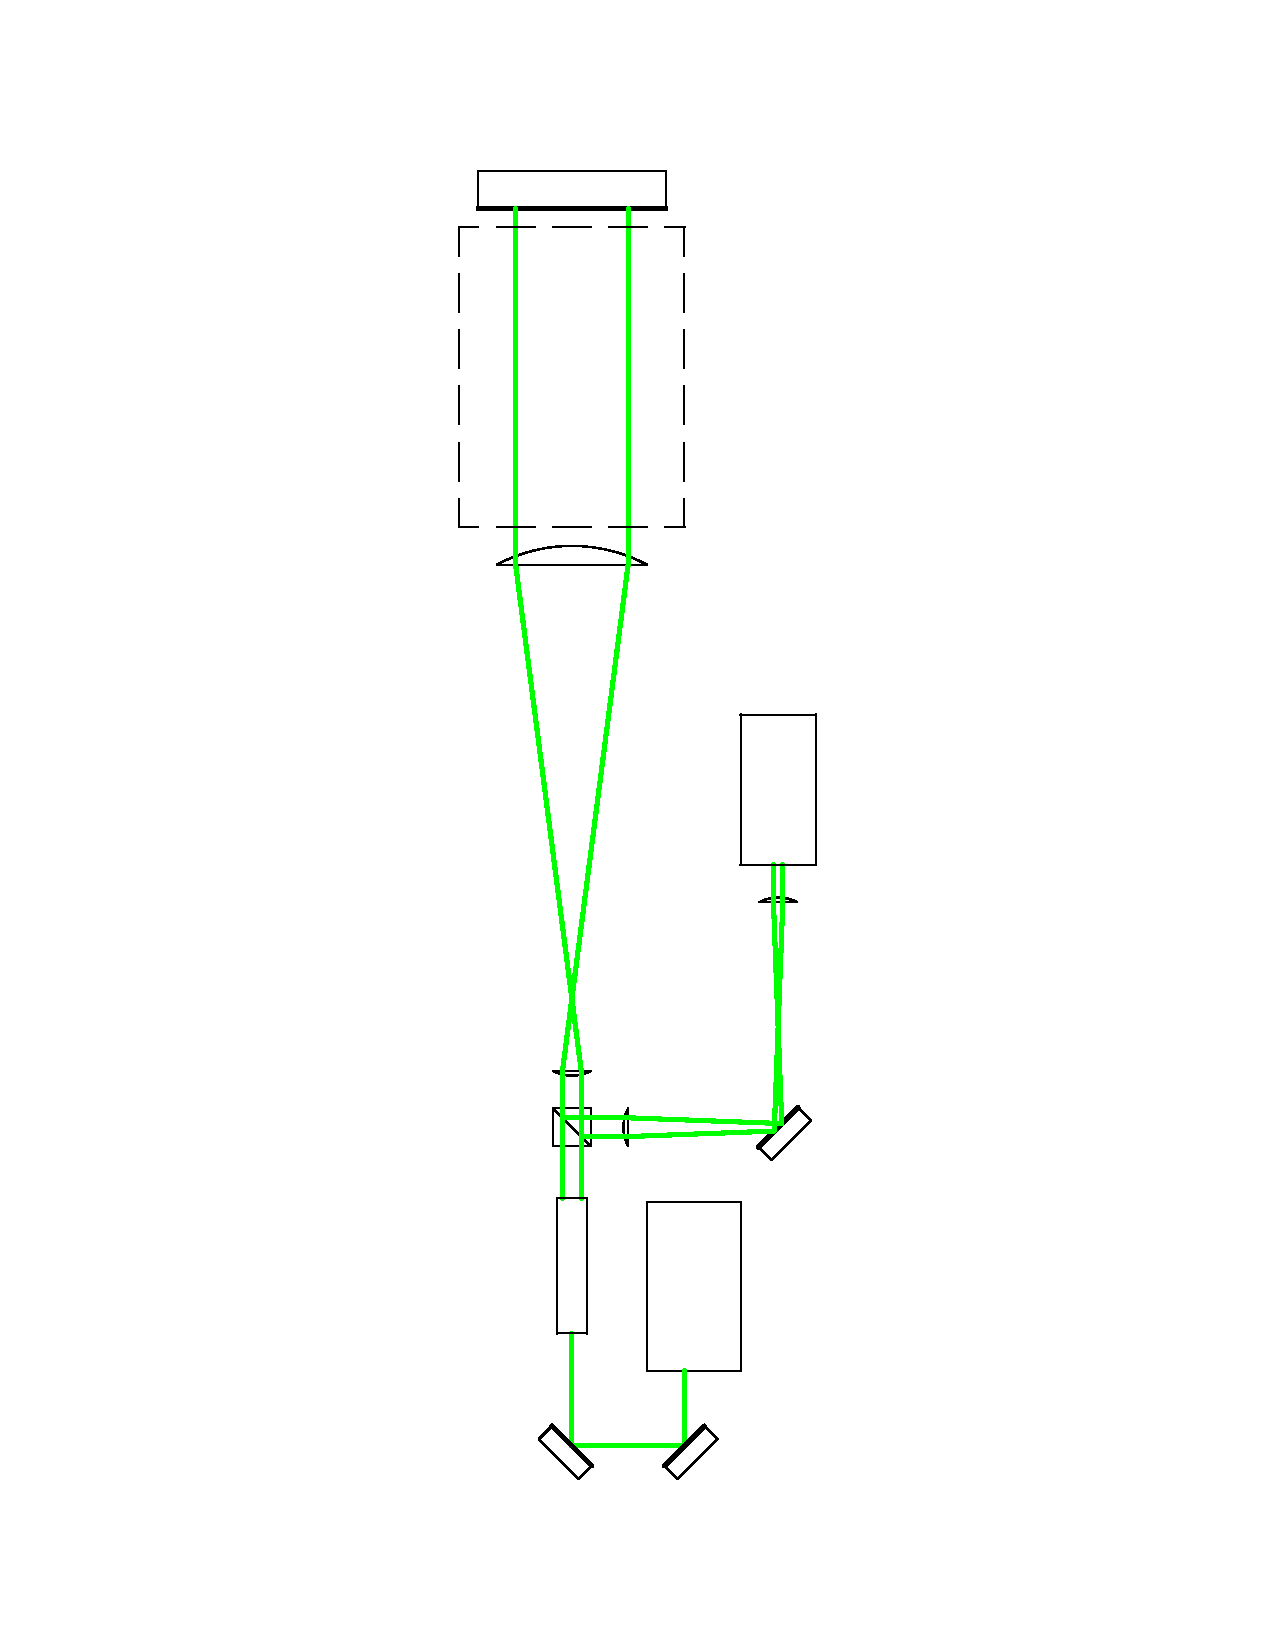
\includegraphics[width=2.5in,clip,trim=200 75 200 75]{../cad/wavefront_setup.pdf}
  \put(-72,62){\rotatebox{90}{\Large LASER}}
  \put(-145,78){\rotatebox{90}{BEAM}}
  \put(-135,65){\rotatebox{90}{EXPANDER}}
  \put(-150,200){\rotatebox{90}{\Large PRIMARY TELESCOPE}}
  \put(-130,400){\rotatebox{90}{\Large MEASUREMENT}}
  \put(-112,427){\rotatebox{90}{\Large REGION}}
  \put(-95,160){\rotatebox{60}{\Large REIMAGING}}
  \put(-80,155){\rotatebox{60}{\Large TELESCOPE}}
  \put(-10,245){\rotatebox{90}{\Large WAVEFRONT}}
  \put(5,260){\rotatebox{90}{\Large SENSOR}}
  \caption{Typical double-pass optical wavefront measurement setup.}
  \label{fig:02_typical_wavefront_system}
\end{figure}




\subsection{A Brief History of Aero-Optics}
The field of aero-optics began with an investigation by Liepmann \cite{Liepmann-1952-89GQ7wyA} into the limits of sensitivity of schlieren systems when used in high-speed flow analysis.
Liepmann used geometric optics to analyze a small-diameter beam and derive its mean-squared fluctuating deflection angle, $\left<\theta^2\right>$.
Liepmann propagated the beam in the $y$ direction and assumed the index of refraction changes in the $x-z$ plane were statistically similar.
Liepmann's analysis for a boundary layer of thickness $\delta$ resulted in
\begin{equation}
  \left<\theta^2\right> = \frac{1}{[n_0(\delta)]^2}\int_0^\delta\int_0^\delta n_0(y)n_0(\zeta)\left<\left(\frac{\partial\nu}{\partial y}\right)^2\right>R_v(|y-\zeta|)dyd\zeta
  \label{eqn:02_liepmann_deflection_angle}
\end{equation}
where the index of refraction is determined from $n=n_0(y)(1+\nu)$ and $R_v(|y-\zeta|)$ is the correlation function for the index variation.
This analysis introduced the concept of a linking equation that allows one to predict time-averaged optical degradation to turbulent flow statistical measurements.

\section{Acoustics}

\subsection{Basic Acoustics}


Starting with the conservation of mass,
\begin{equation}
  \frac{\partial\rho}{\partial t}+\nabla\cdot\left(\rho\mathbf{u}\right)=0  \textrm{,}
  \label{eqn:02_cons_of_mass}
\end{equation}
and separating the density into a time-averaged ($\rho_0$) and fluctuating portion ($\rho'$), $\rho = \rho_0+\rho'$.
The fluctuating conservation of mass equation is obtained by separating the density ($\rho = \rho_0+\rho'$) into a temporally averaged density, $\rho_0$, and a

\begin{equation}
  \frac{\mathbf{D}\rho'}{\mathbf{Dt}}+\nabla\cdot\left(\rho_0\mathbf{u}\right)=0
  \label{eqn:02_cons_of_mass_fluc}
\end{equation}





For acoustics waves of frequency less than $10^9$ Hz the compression of the fluid can be assumed to be adiabatic \cite{Morse-1968-yygEdQZf}.


\begin{equation}
  \left.\frac{\partial p}{\partial\rho}\right|_s = c_0^2
  \label{eqn:02_speed_of_sound}
\end{equation}

\subsection{Duct Acoustics}
Acoustic waves are often enclosed inside of somesort of structure.
This section will look at acoustics when confined to a duct in which the acoustic waves primarily travel along one-axis and have walls confining the acoustics along the other two axes as is the case inside of a wind tunnel.
Figure \ref{fig:02_duct_drawing} shows the diagram used for deriving the acoustic properties inside of a constant area duct.
\begin{figure}
\centering
  % \fbox{
    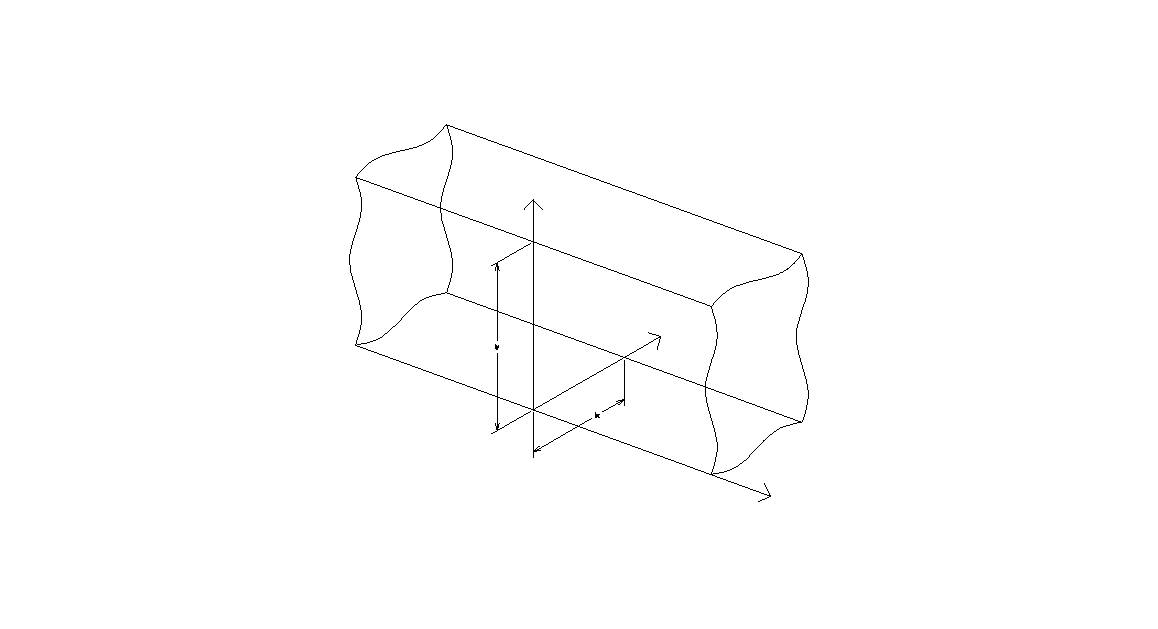
\includegraphics[trim=2.2in 0.7in 2.2in 0.7in,clip,width=4.5in]{../autocad/02_background/duct_drawing.eps}
    \put(-155,62){\fcolorbox{white}{white}{$l_x$}}
    \put(-227,113){\fcolorbox{white}{white}{$l_y$}}
    \put(-103,119){$\mathbf{x}$}
    \put(-198,220){$\mathbf{y}$}
    \put(-26,4){$\mathbf{z}$}
  % }
  \caption{Duct with a rectangular cross-section.}
  \label{fig:02_duct_drawing}
\end{figure}

This derivation is primarily influenced from Munjal \cite{Munjal-2014-w28y4EyP} along with Jacobsen and Juhl \cite{Jacobsen-2013-PHD3v3YZ}.
The primary assumption used in this derivation is that the duct is of constant cross-section.
This means that all mean quantities ($\rho_0$, $\mathbf{u_0}$, ...) a constant throughout space and time.
Starting with the linearized inviscid forms of the conservation of mass,
\begin{equation}
  \frac{\mathbf{D}\rho}{\mathbf{Dt}} + \rho_0\nabla\cdot\mathbf{u} = 0 \textrm{,}
  % \frac{\partial\rho}{\partial t} + \mathbf{u}\cdot\nabla\rho + \rho_0(\nabla\cdot\mathbf{u}) = 0 \textrm{,}
  \label{eqn:02_cons_mass}
\end{equation}
and conservation of momentum,
\begin{equation}
  \rho_0\frac{\mathbf{Du}}{\mathbf{Dt}} + \nabla p = 0 \textrm{.}
  % \rho_0\frac{\partial\mathbf{u}}{\partial t} + \rho_0(\mathbf{u_0}\cdot\nabla)\mathbf{u} + \nabla p = 0 \textrm{.}
  \label{eqn:02_cons_mom}
\end{equation}
The definition of the speed of sound (Equation \ref{eqn:02_speed_of_sound}) is then substituted into Equation \ref{eqn:02_cons_mass},
\begin{equation}
  \frac{1}{c_0^2}\frac{\mathbf{D}p}{\mathbf{Dt}} + \rho_0\nabla\cdot\mathbf{u} = 0 \textrm{,}
  % \frac{1}{c_0^2}\frac{\partial p}{\partial t} + \frac{1}{c_0^2}(\mathbf{u}\cdot\nabla p) + \rho_0(\nabla\cdot\mathbf{u}) = 0 \textrm{,}
  \label{eqn:02_cons_mass_p}
\end{equation}
where $c_0$ is the speed of sound at average fluid properties ($\rho_0$, $p_0$, $T_0$, ...).
Next the difference between the material derivative ($\mathbf{D}/\mathbf{Dt}$) of Equation \ref{eqn:02_cons_mass_p} and the partial derivative ($\partial/\partial\mathbf{x}$) of Equation \ref{eqn:02_cons_mom} with respect to space is taken which results in the convected 3-D wave equation,
\begin{equation}
  \left(\frac{\mathbf{D}^2}{\mathbf{Dt}^2}-c_0^2\nabla^2\right)p=0\textrm{.}
  \label{eqn:02_wave_conv_3_c}
\end{equation}
Expanding the material derivative and dividing by $c_0^2$,
\begin{equation}
  \left(\frac{1}{c_0^2}\frac{\partial^2}{\partial t^2} + \frac{2\mathbf{M}}{c_0}\frac{\partial^2}{\partial t\partial\mathbf{x}} - (1-\mathbf{M}^2)\nabla^2\right)p = 0 \textrm{,}
  \label{eqn:02_wave_conv_expand}
\end{equation}
where $\mathbf{M} = \mathbf{u_0}/c_0$.
By using the fact that $c_0=\omega/k_0$, Equation \ref{eqn:02_wave_conv_3_c} can be written in a more convent form,
\begin{equation}
  \left(\frac{1}{\omega^2}\frac{\partial^2}{\partial t^2} + \frac{2\mathbf{M}}{\omega k_0}\frac{\partial^2}{\partial t\partial\mathbf{x}} - \frac{1-\mathbf{M}^2}{k_0^2}\nabla^2\right)p = 0 \textrm{,}
  \label{eqn:02_wave_conv_3}
\end{equation}
where $\omega$ is the angular frequency and $k_0$ is the total wavenumber.

At this point the pressure field is going to written in a complex form and assumed to be separable in both time and space such that $\hat{p}(\mathbf{x},t) = \hat{p}(x,y)\hat{p}(z)\hat{p}(t)$.
The temporal solution is assumed to take the form
\begin{equation}
  \hat{p}(t) = \exp\left\{j\omega t\right\} \textrm{.}
  \label{eqn:02_pressure_solution_time}
\end{equation}
This results in the spatial component of the convecting wave equation
\begin{equation}
  \left((1-\mathbf{M}^2)\nabla^2-2jk_0\mathbf{M}\nabla+k_0^2\right)\hat{p}(x,y)\hat{p}(z) = 0 \textrm{.}
  \label{eqn:02_wave_conv_space}
\end{equation}
This can be further split into axial and cross-sectional components by splitting $k_0$ into components,
\begin{equation}
  k_0 = \sqrt{k_{xy}^2+k_z^2} \textrm{,}
  \label{eqn:02_k0}
\end{equation}
and because the mean flow is only in the axial direction ($\mathbf{M} = M\mathbf{\hat{k}}$).
The cross-sectional component is a typical Helmholtz equation
\begin{equation}
  \left(\frac{\partial^2}{\partial x^2}+\frac{\partial^2}{\partial y^2}\right)\hat{p}_{xy}(x,y)+k_{xy}^2\hat{p}(x,y) = 0 \textrm{,}
  \label{eqn:02_wave_xy}
\end{equation}
whos solution,
\begin{equation}
  \hat{p}(x,y) = \Psi_m(x,y) \textrm{,}
  \label{eqn:02_pressure_solution_xy}
\end{equation}
is one of infinity many eigen-function solutions with discrete wavenumbers, $k_m$.
The axial component of the convecting wave equation,
\begin{equation}
  (1-M^2)\frac{\partial^2\hat{p}(z)}{\partial z^2} - 2jk_0M\frac{\partial\hat{p}(z)}{\partial z} + k_z^2\hat{p}(z) = 0 \textrm{,}
  \label{eqn:02_wave_z}
\end{equation}
retains the total wavenumber in second term which means its solution will depend on the cross-sectional wavenumber value at cross-sectional mode.
The solution to the axial convecting wave equation,
\begin{equation}
  \hat{p}(z) = p^+_m\exp{\left\{-jk^+_{zm}z\right\}}+p^-_m\exp{\left\{+jk^-_{zm}z\right\}} \textrm{,}
  \label{eqn:02_pressure_solution_z}
\end{equation}
has waves traveling in both directions with the axial wavenumber in each direction for a given mode
\begin{equation}
  k^\pm_{zm} = \frac{\mp Mk_0+\sqrt{k_0^2-(1-M^2)k_m^2}}{1-M^2} \textrm{.}
  \label{eqn:02_kzm}
\end{equation}

The solution for a three-dimensional acoustic wave in a duct with a constant but arbitrary cross-section in complex pressure is the combination of the component solutions presented in Equations \ref{eqn:02_pressure_solution_time}, \ref{eqn:02_pressure_solution_xy}, and \ref{eqn:02_pressure_solution_z},
\begin{equation}
  \hat{p}(x,y,z,t) = \Psi_m(x,y)\left(p^+_m\exp{\left\{-jk^+_{zm}z\right\}}+p^-_m\exp{\left\{+jk^-_{zm}z\right\}}\right)\exp\left\{j\omega t\right\} \textrm{.}
  \label{eqn:02_pressure_solution_duct}
\end{equation}
The two solutions for a plane wave ($\Psi_m=1$, $k_m=0$) traveling in a duct have a characteristic speed of $u\pm c_0$.
Acoustic modes will travel indefinitly if $k_0^2-(1-M^2)k_m^2>0$ (the quantity inside of the square-root of Equation \ref{eqn:02_kzm}).
This presents a frequency at which a given mode will cut-on,
\begin{equation}
  f_{cuton} = \frac{c_0}{2\pi}\sqrt{(1-M^2)k_m^2} \textrm{.}
  \label{eqn:02_cuton_freq}
\end{equation}
Below this frequency, an acoustic mode will be exponentially attenuated as it travels throught the duct.

\subsubsection{Characteristic Equations of Cross-Sections}
In order to determine the characteristic equations of an acoustic field within a cross-section the solution to Equation \ref{eqn:02_wave_xy} needs to be determined.
A typical boundary condition that is used in the solution of this 2-D Helmholtz equation is using the assumption that the walls are rigid.
\begin{equation}
  \nabla p_{x,y}(x,y)\cdot\mathbf{n}_{wall} = 0
  \label{eqn:02_bc_rigig_wall}
\end{equation}
This boundary condition results in the acoustic waves being perfectly reflected off of the duct walls.
There are several known empirical solution sets of the characteristic equations for specific geometry with the rigid wall assumption.

The first of these solutions is for a rectangular cross-section,
\begin{equation}
  \Psi_{m,n}(x,y) = \cos(k_xx)\cos(k_yy) \textrm{,}
  \label{eqn:02_psi_rect}
\end{equation}
where the wave numbers along each axis are $k_x = m\pi/l_x$ and $k_y = n\pi/l_y$.
The duct has a width of $l_x$ and a height of $l_y$.
The total cross-sectional wave number for use in determining the axial wave numbers is
\begin{equation}
  k_m^2 = k_x^2+k_y^2 \textrm{.}
  \label{eqn:02_wave_number_crosssection}
\end{equation}
Figure \ref{fig:02_cross_section_rect} shows the characteristic functions when m=0:2 and n=0:3 for a rectangular cross-section of width of $l_x$ and height of $l_y$.
\begin{figure}
  \centering
  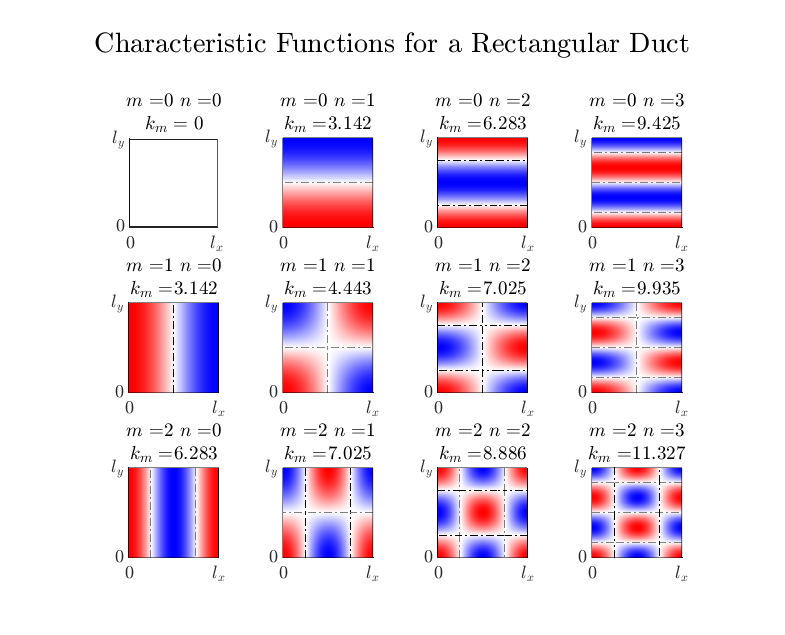
\includegraphics{../matlab/02_background/cross_section_rect.eps}
  \caption{Characteristic solutions to Equation \ref{eqn:02_wave_xy} with rigid wall in a rectangular cross-section where m=0:2 and n=0:3.  Nodal lines are depicted by the dot-dash lines.  The cross-sectional wave numbers, $k_m$, listed are for a duct of unit length and height.}
  \label{fig:02_cross_section_rect}
\end{figure}
The lines depicted in the figure are nodal lines and represent locations where there is zero pressure fluctuations for that acoustic mode.

The second set of known empirical solutions is for a circular cross-section with radius $R$,
\begin{equation}
  \Psi_{m,n}(r,\theta) = J_m(k_{mn}r)\exp\left\{\pm jm\theta\right\} \textrm{,}
  \label{eqn:02_psi_circ}
\end{equation}
where $J_m$ is the $m^\textrm{th}$ Bessel function of the first kind and the $\pm$ indicates the direction of spin.
If the left and right spin coefficients are equal in magnitude then a non-spinning mode is created.
In order to satisfy the solid wall boundary condition $J_m'(k_{mn}R) = 0$ which determines a set of discrete values for the cross-sectional wave number at the $n^\textrm{th}$ zero for the $m^\textrm{th}$ Bessel function.
Figure \ref{fig:02_cross_section_circ} shows the characteristic functions for a circular duct.
\begin{figure}
  \centering
  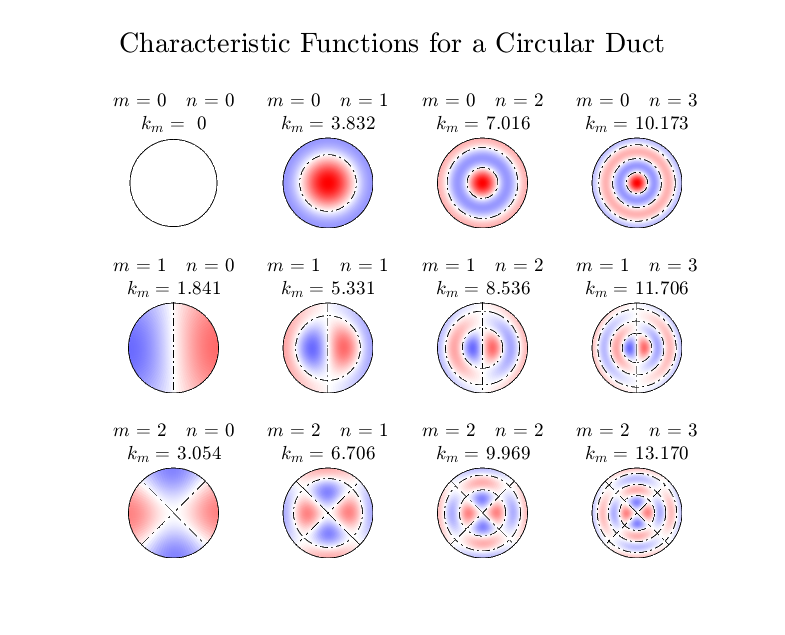
\includegraphics{../matlab/02_background/cross_section_circ.eps}
  \caption{Characteristic solutions to Equation \ref{eqn:02_wave_xy} with rigid wall in a circular cross-section where m=0:2 and n=0:3.  Nodal lines are depicted by the dot-dash lines.  The cross-sectional wave numbers, $k_m$, listed are for a duct of unit radius.}
  \label{fig:02_cross_section_circ}
\end{figure}

    % !TEX root = catron-dissertation.tex
\epstopdfsetup{outdir=./images/03_aero_optics_acoustics/}

\chapter{Aero-Optical and Acoustical Coupling}
\label{chap:03}

\begin{itemize}
  \color{red}
  \item Spherical solutions and measurements
  \item Double check microphone and preamp models and settings
  \item Mode marching method
\end{itemize}


Acoustic waves are isentropic compression waves with the fluctuating pressure, $p'$, determining the strength of the wave.
This fluctuating pressure is related to the sound pressure level, $\spl$ by
\begin{equation}
  \spl = 20\log_{10}\left(\frac{p_{rms}}{p_0}\right)
  \label{eqn:03_spl}
\end{equation}
where $p_{rms}$ is the root mean square of the pressure fluctuation, and $p_0$ is the reference pressure (20 $\mu$Pa for air).
The pressure fluctuations can be converted to the density fluctuations via the definition of the speed of sound:
\begin{equation}
  c_0^2 = \left(\frac{\partial p}{\partial \rho}\right)_s=\frac{p'}{\rho'}
  \label{eqn:03_speed_sound}
\end{equation}
where $c_0$ is the speed of sound at mean fluid properties and the subscript $s$ denotes constant entropy.
It can be shown by combining Equations \ref{eqn:02_gladstone_dale_relation_fluctuating} and \ref{eqn:02_opd} that the fluctuating density can be related to the $\opd$,
\begin{equation}
  \opd = K_{GD}\int_{s_1}^{s_2}{\rho'}ds \textrm{.}
  \label{eqn:03_opd_fluct}
\end{equation}
This can be combined with Equation \ref{eqn:03_speed_sound},
\begin{equation}
  \opd = \frac{K_{GD}}{c_0^2}\int_{s_1}^{s_2}{p'}ds \textrm{,}
  \label{eqn:03_opd_pressure}
\end{equation}
to provide a way of computing the optical path difference of a pressure field.

% When the pressure field is known in complex quantities (magnitude and phase), a complex optical path difference can calculated,

% Here the complex pressure field was assumed to be seperable in time and space.
% The measurable $\opd$ is

% This can greatly reduce the computational cost of simulating a beam passing through a pressue or density field that is separable in time and space by only performing the spatial integration once for each temporal frequency component.

\section{Simulating an Optical Wavefront Measurement from an Acoustic Field Function}
\label{chap:03_simulated_beam}
An optical wavefront can be simulated from a complex pressure field by applying Equation \ref{eqn:03_opd_pressure}.
To accomplish this, two separate coordinate systems will need to be defined.
The first is the beam coordinate system, $\mathbf{x}_B $, that will have a measurement aperture, which is typically circular, defined in the xy-plane and propagates in the z-direction.
The second is the acoustic coordinate system, $\mathbf{x}_A$, that will be defined based on the source location or the geometry that the acoustic waves are propagating through.
These to coordinate systems will have a function representing a transform from one to the other
\begin{equation}
  \mathbf{x}_A = R\mathbf{x}_B+T \textrm{,}
  \label{eqn:03_coord_transform}
\end{equation}
where $R$ is a matrix which represents the rotation and $T$ is a vector that represents the translation.

The important parameters for defining the aperture which the beam coordinate system is based are the aperture size, $Ap$, and the number of lenslets or sub-apertures, $N_{lenslets}$.
Assuming that the aperture is either circular or square and the lenslet size and sub-aperture size is approximately $Ap/N_{lenslets}$, the x locations of the center of the sub-apertures go from $-Ap/2(1-1/N_{lenslets})$ to $Ap/2(1-1/N_{lenslets})$ by steps of $Ap/N_{lenslets}$ with the y locations having the same values.
This gives a matrix representing both $x_{Ap}$ and $y_{Ap}$ that is $N_{lenslets}$ by $N_{lenslets}$.
For the purpose of removing piston, tip, and tilt and creating a mask that represents the beam aperture, the radial coordinates, $\rho_{Ap}$ and $\theta_{Ap}$, of the aperture should also be calculated.
A circular beam will have a mask defined by,
\begin{equation}
  Mask_{Ap} =
  \begin{cases}
    1, & \text{if } \rho_{Ap}\leq Ap/2 \\
    0, & \text{otherwise.}
  \end{cases}
\end{equation}
The beam coordinate frame is the aperture coordinates extruded in the z-direction over the range of desired z-values.

After the beam coordinates are transformed into the acoustic coordinates using Equation \ref{eqn:03_coord_transform}, the complex pressure field, $\hat{p}(x,y,z,t)$ can be calculated at the points that are within the optical beam.
If the pressure field is separable into spatial and temporal components, than the integration along the beam length only needs to be done once for each temporal frequency,
\begin{equation}
  \widehat{\opd}(x,y) = \frac{K_{GD}}{c_0^2}\int_{z_1}^{z_2} \hat{p}(x,y,z)_{Ap}dz \textrm{,}
  \label{eqn:03_opd_complex}
\end{equation}
where $\widehat{\opd}(x,y)$ is the complex optical path difference as measured in the aperture plane.
If a complex density field is known instead, than Equation \ref{eqn:03_opd_complex} becomes
\begin{equation}
  \widehat{\opd}(x,y) = K_{GD}\int_{z_1}^{z_2} \hat{\rho}(x,y,z)_{Ap}dz \textrm{.}
  \label{eqn:03_opd_complex_density}
\end{equation}
For the purposes of calculating temporally mean optical properties of simulated beam passing through a known complex pressure or density field a phase vector was defined,  $\phi = [0, 2\pi)$.
The measurable component as a function of phase is
\begin{equation}
  \opd(x,y,\phi) = \real\left[\widehat{\opd}(x,y)\exp\{-j\phi\}\right] \textrm{,}
  \label{eqn:03_opd_real_phase}
\end{equation}
or as a function of time for all temporal frequencies,
\begin{equation}
  \opd(x,y,t) = \real\left[\sum\widehat{\opd}(x,y)\exp\{-j\omega t\}\right] \textrm{,}
  \label{eqn:03_opd_real}
\end{equation}
where there is a separate $\widehat{\opd}(x,y)$ computed for each temporal frequency.
One of the more important measurements that can be calculated from $\opd$ is the spatial RMS, $\opdrms$, which is calculated at each time or phase step at the points where the aperture mask equals one.

\section{Simple Examples of Acoustic-Optical Coupling}
Two basic acoustic pressure fields will be numerically examined for their optical properties.
The first will be a planar acoustic wave that will be numerically simulated over a variety of conditions.
The second will be a spherical acoustic wave that will be both numerically simulated and validated experimentally.

\subsection{Planar Acoustic Waves}
A planar wave is the simplest solution to the wave equation and varies only in time and the direction of travel.
A planar wave can be calculated from the set of solutions for duct acoustics, Equation \ref{eqn:02_pressure_solution_duct}, given that $\Psi_m(x,y)=1$,
\begin{equation}
  \hat{p}(z,t) = p_m\exp\left\{j(\omega t \mp k_{zm}^\pm z)\right\} \textrm{.}
  \label{eqn:03_plane_wave}
\end{equation}
This section will show several plots to show the effect that acoustic waves have on the optical wavefront of a planar wave with the general geometry shown in Figure \ref{fig:03_planar_sample_domain}.
\begin{figure}
  \centering
  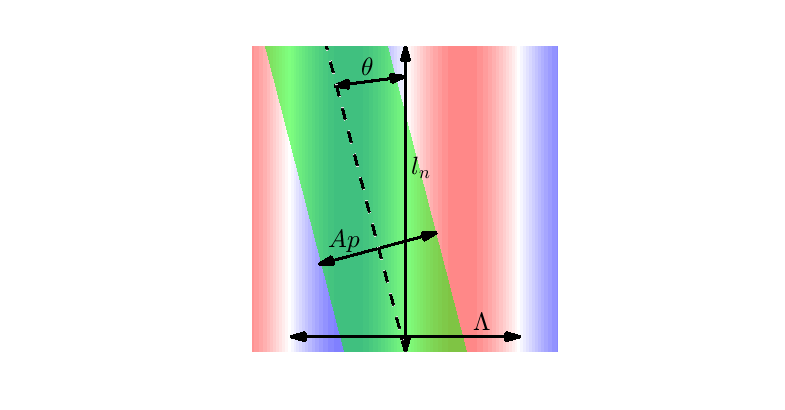
\includegraphics{../matlab/03_aero_optics_acoustics/planar_sample_domain.eps}
  \caption{General geometry for various sample calculations for showing the acoustic-optical coupling effect.}
  \label{fig:03_planar_sample_domain}
\end{figure}
For the following example, $l_n$ is the width of the acoustic disturbance (for example, the width of the wind tunnel), $\theta$ is the angle between the planar acoustic wave and the beam direction, $A_p$ is the aperture diameter of the beam, and $\Lambda$ is the wavelength of the acoustic wave.

Figure \ref{fig:03_planar_sample_calc_3} shows the time averaged $\opdrms$ per meter of beam propagation when the beam path is parallel ($\theta=0$) to the peaks and troughs of the planar acoustic wave as $\spl$ is varied.
\begin{figure}
  \centering
  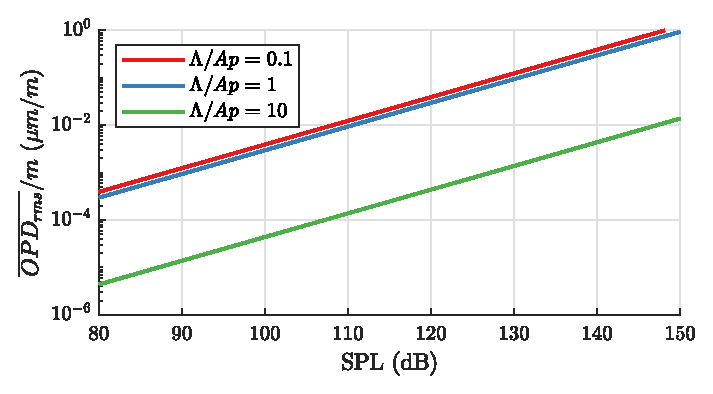
\includegraphics{../matlab/03_aero_optics_acoustics/planar_sample_calc_3.eps}
  \caption{Theoretical time-averaged $\opdrms$ per meter of beam propagation as a function of sound pressure level, $\spl$, for several $\Lambda/Ap$ ratios and $\theta=0$.}
  \label{fig:03_planar_sample_calc_3}
\end{figure}
As the sound pressure level increases the time averaged $\opdrms$ also increases and can easily reach the point of being a significant factor in the measured optical disturbance.
There is little difference between 0.1 and 1 $\Lambda/Ap$, but as the wavelength gets much larger compared to the beam diameter, then the optical effect of the noise is greatly reduced, this effect is known as aperture filtering \cite{Siegenthaler-2005-KQ2HGmfp}.

Aperture filtering is more clearly shown in Figure \ref{fig:03_planar_sample_calc_1}.
\begin{figure}
  \centering
  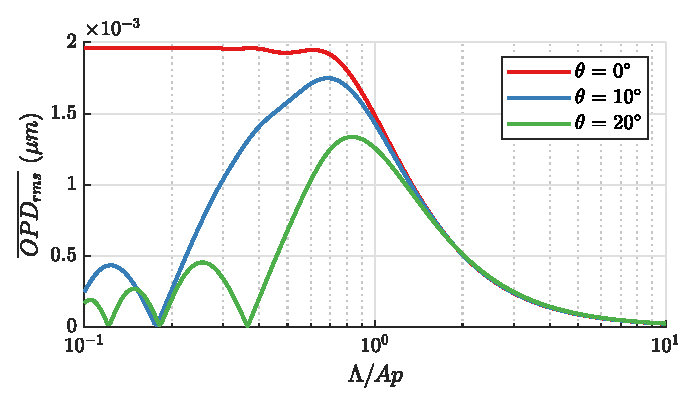
\includegraphics{../matlab/03_aero_optics_acoustics/planar_sample_calc_1.eps}
  \caption{Theoretical time-averaged $\opdrms$ for a rms sound pressure of 1 Pa ($\spl$ of 94 dB), $l_n$ of 1 m, and various angles and $\Lambda/Ap$ ratios.}
  \label{fig:03_planar_sample_calc_1}
\end{figure}
As the $\Lambda/Ap$ ratio increases from 0.1, time-averaged $\opdrms$ remains fairly constant until it starts to drop around $\Lambda/Ap$ of 0.7 and starts to asymptotically approach zero which it basically reaches by $\Lambda/Ap$ of 10.
Figure \ref{fig:03_planar_sample_calc_1} also shows the effect of changing the beam angle, $\theta$, through the acoustic field.
For nonzero $\theta$, the beam encounters alternating high and low index of refraction as it passes through the test region, so that the time-averaged $\opdrms$ begins to decrease compared to the $\theta = 0^\circ$ case below $\Lambda/Ap=1$.
There are also points of zero optical disturbance that occur at $\theta_{zero}=\tan^{-1}(n\Lambda/l_n)$ for $n\neq0$; these points occur because the peaks and valleys of the optical disturbance caused by the sound wave effectively cancel out over the length of the integration path, $l_n/\cos\theta$.

Figures \ref{fig:03_planar_sample_calc_3} and \ref{fig:03_planar_sample_calc_1} show the optical effect of plane acoustic waves in a no-flow environment.
The effect of wind-tunnel flow is to stretch (downstream-traveling waves) or compress (upstream-traveling waves) the wavelength of the acoustic noise thereby altering the filtering effect of the beam aperture.
Figure \ref{fig:03_planar_sample_calc_2} shows a typical optical disturbance from the two transverse acoustic waves (u+c and u-c) present in a wind tunnel at Mach 0.6.
\begin{figure}
  \centering
  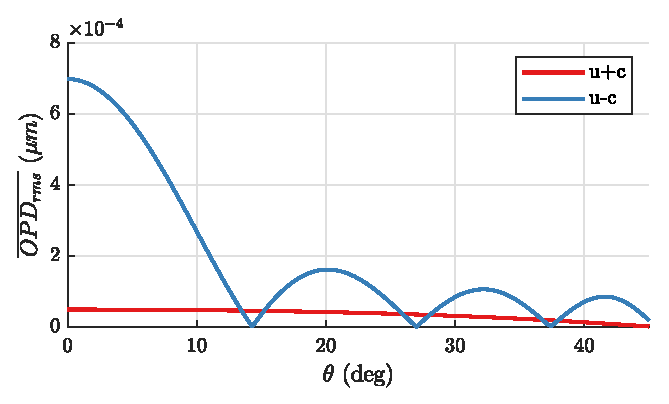
\includegraphics{../matlab/03_aero_optics_acoustics/planar_sample_calc_2.eps}
  \caption{Theoretical time-averaged $\opdrms$ for the two acoustic waves (u+c and u-c) for the blade pass frequency (534 Hz) at Mach 0.6 with a RMS sound pressure of 1 Pa ($\spl$ of 94 dB), $l_n$ of 1 m, and $Ap$ of 15 cm.}
  \label{fig:03_planar_sample_calc_2}
\end{figure}
Both waves have a RMS sound pressure of 1 Pa and the beam has an aperture of 15 cm and propagates through a 1 m acoustic field inside the tunnel.
Over a vast majority of the look back angles the upstream-traveling acoustic wave has a much greater effect on the optical disturbance compared to the downstream-traveling acoustic wave, due to the much shorter wavelength of the upstream-traveling waves which is less affected by aperture filtering.
However, the upstream-traveling wave goes through several zero points so the downstream-traveling wave dominates at some look back angles.

% In summary, Figures \ref{fig:03_planar_sample_calc_3} to \ref{fig:03_planar_sample_calc_2} give an example of how planar acoustic waves are expected to affect a beam traveling a finite distance $l_n$ at an angle $\theta$ through the acoustic field.

\subsection{Spherical Acoustic Waves}
The acoustic field from an speaker maybe assumed to be a spherical wave from a pulsating point if the frequency is sufficiently low and measurement region is far enough away from the source \cite{Randall-1951-9NtPPXPq}.
This pressure field when converted to complex pressure is represented by
\begin{equation}
  \hat{p}(r,t) = \frac{A_0}{r}\exp\left\{-j(kr-\omega t)\right\} \textrm{,}
  \label{eqn:03_spherical_pressure}
\end{equation}
where $A_0$ is the fluctuating pressure strength and $r$ is the distance from the source to the measurement point.
The RMS pressure of this field can be represented by
\begin{equation}
  p_{rms} = \frac{|A_0|}{r\sqrt{2}} \textrm{.}
  \label{eqn:03_spherical_pressure_rms}
\end{equation}

\subsubsection{Theoretical OPD Measurements}
A set of optical properties where calculated for a beam passing through a spherical acoustic field as defined by a point source using the process discribed previously in Chapter \ref{chap:03_simulated_beam}.
These calculations used an circular aperture size of 0.25-m in diameter consisting of 32x32 sub-apertures, an acoustic wavelength, $\Lambda$, of $Ap/4$ to $10Ap$, and a distance from the point source to the center of the aperture, $R$, of $5Ap$ to $25Ap$.
The beam was integrated over $\pm5$-m from the plane of the point source with 25 phase step used to calculate mean values.

The result of these simulated acoustic fields is shown in Figure \ref{fig:03_spherical_sample}.
\begin{figure}
  \centering
  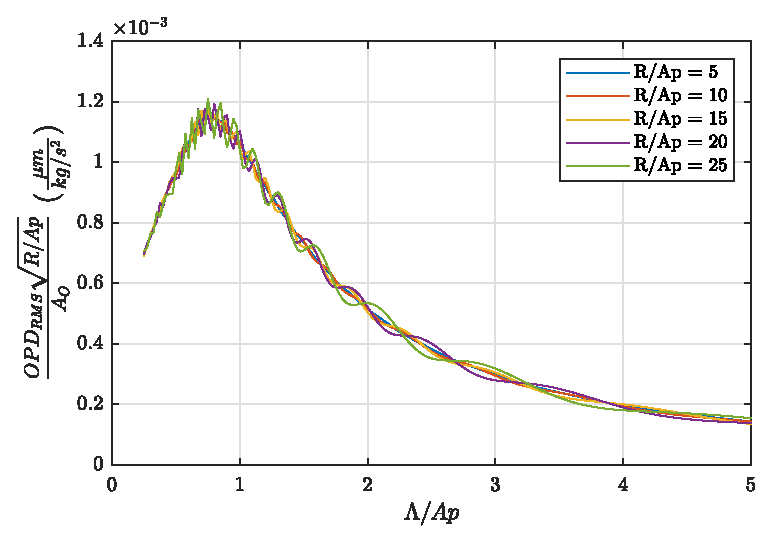
\includegraphics{../matlab/03_aero_optics_acoustics/spherical_sample.eps}
  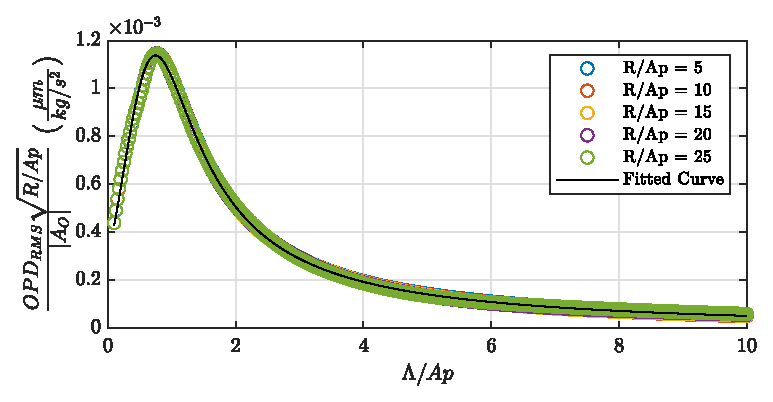
\includegraphics{../matlab/03_aero_optics_acoustics/spherical_sample_win.eps}
  \caption{Theoretical time-averaged $\opdrms$ for a spherical acoustic wave. The top plot shows a perfect spherical acoustic signal integrated over $\pm$5-m. The bottom plot shows has a Tukey window applied along the beam length to partially emulate source directivity which significantly reduces the measured oscillations.}
  \label{fig:03_spherical_sample}
\end{figure}
The top plots shows the expected optical disturbance ratio, $\opdrms/|A_0|$, for a perfectly spherical acoustic field measured over the beam length.
With the exception of some oscillations that are caused by end effects in the integration.
The oscillations can be greatly reduced by using a windowing function in the z-direction such as a Hanning or Tukey window which also can be used to roughly model directivity of the speaker's acoustic emission as shown in the bottom plot.
While this plot was calculated with a single aperture diameter, the general trend holds for all other aperture diameters that were tested, the only effect was the size and width of the oscillations.

The peak of the optical disturbance ratio, $\opdrms/|A_0|$, is located at $\Lambda/Ap\approx0.75$ for a circular aperture.
The signal is reduced above this value due to aperture filtering and below this value because the shorter wavelength have a reduced distance before alternating high and low index-of-refraction regions reduce the optical path difference.
When the acoustic source point is sufficiently far enough away from the measurement beam, $R/Ap\geq2$, the optical disturbance ratio, $\opdrms/|A_0|$ when multiplied by $\sqrt{R/Ap}$, can be collapsed onto a single curve for a range of $\Lambda/Ap$ of 0.1 to 10.
Above $\Lambda/Ap=10$ the curves start to diverge away from one another.
An approximate function fit to this data is
\begin{equation}
  \frac{\opdrms\sqrt{R/Ap}}{|A_0|} \approx \frac{p_1(\Lambda/Ap)^3+p_2(\Lambda/Ap)^2+p_3(\Lambda/Ap)+p_4}{(\Lambda/Ap)^3+q_1(\Lambda/Ap)^2+q_2(\Lambda/Ap)+q_3}
  \label{eqn:03_spherical_sample_fit}
\end{equation}
with coefficient values shown Table \ref{tab:03_speherical_sample_coeff}.
This functional fit has a $R^2$ value of 0.9991.
\begin{table}
\centering
\caption{Curve fit values for Figure \ref{fig:03_spherical_sample} and Equation \ref{eqn:03_spherical_sample_fit}}
\input{../matlab/03_aero_optics_acoustics/spherical_sample_win.txt}
\label{tab:03_speherical_sample_coeff}
\end{table}


\subsubsection{Measurement of a Spherical Acoustic Wave with an Optical Beam}
A small benchtop experiment was used to compare the simultaious optical and microphone measurements of an acoustic field from a speaker as shown in the measurement plane in Figure \ref{fig:03_speaker_test}.
\begin{figure}
  \centering
  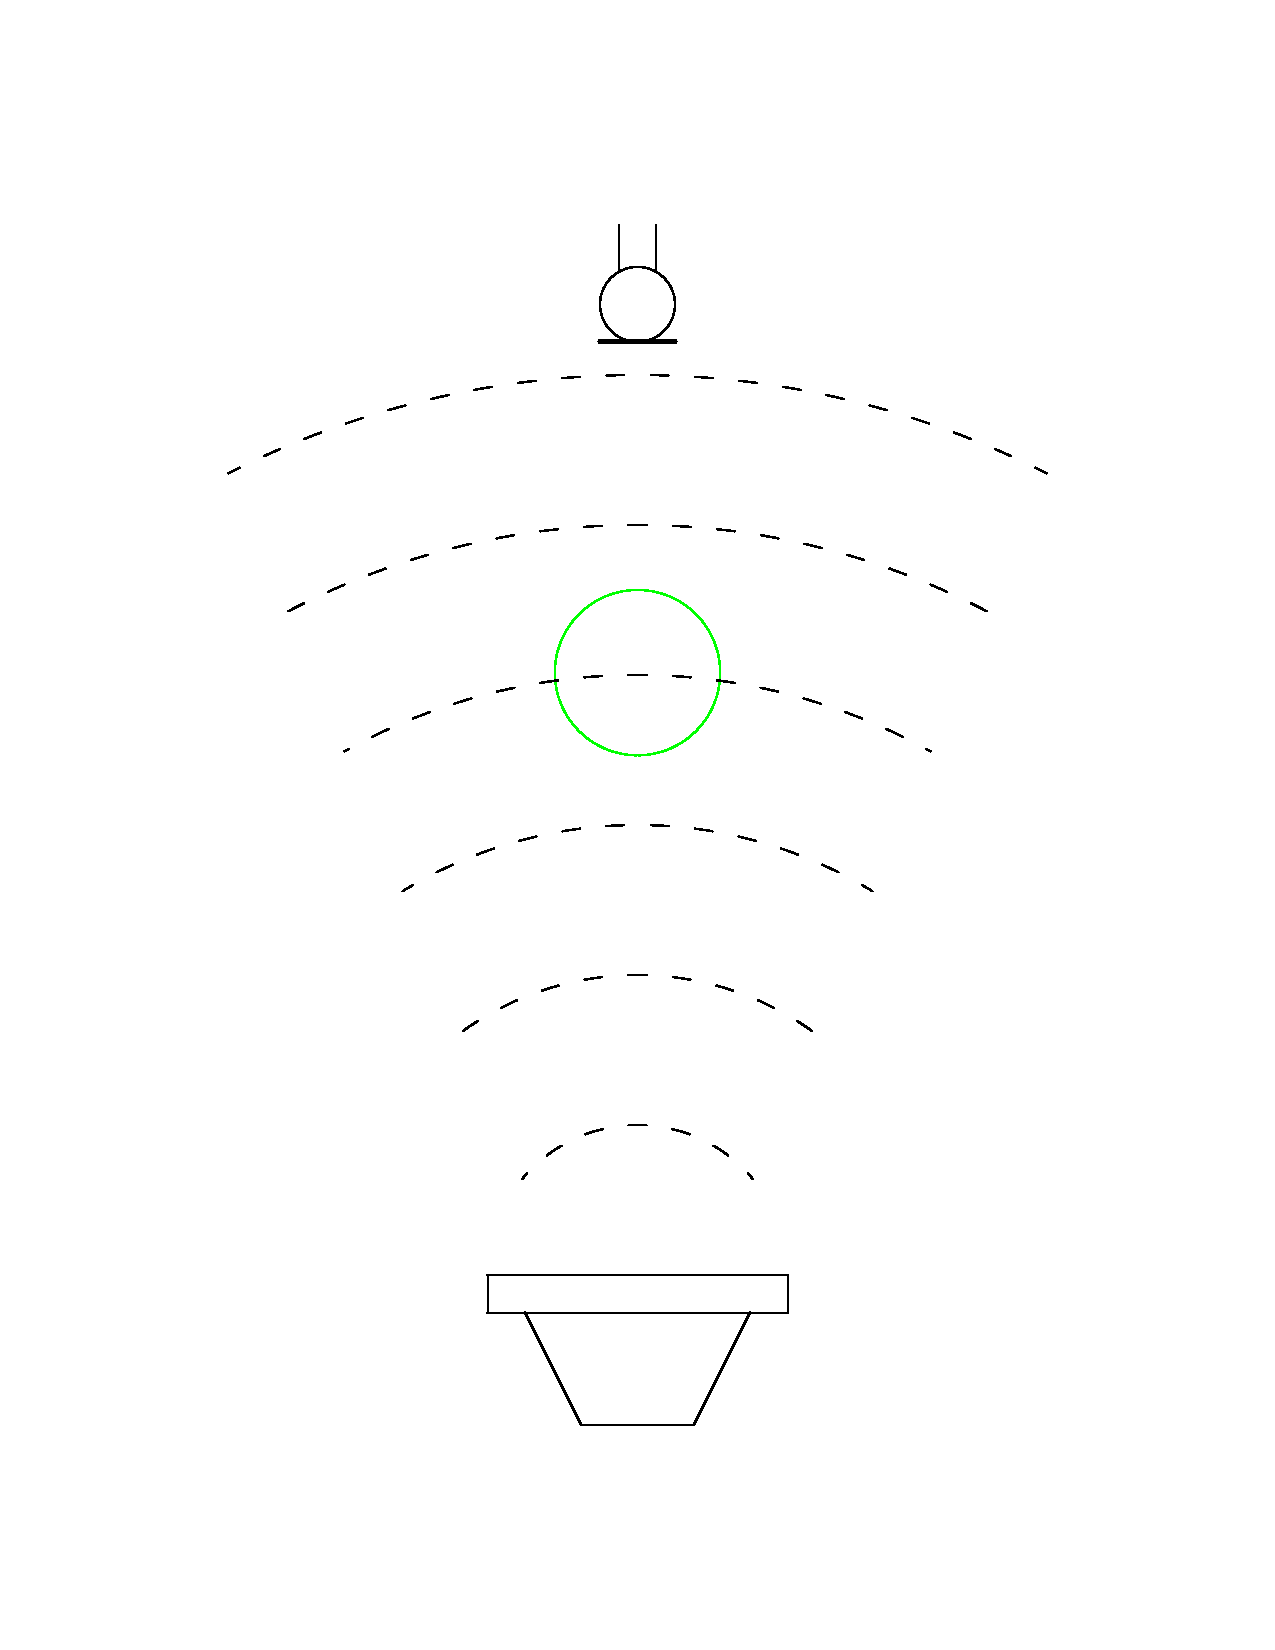
\includegraphics[width=3.5in,clip,trim=100 100 100 100]{../cad/speak_test.pdf}
  \caption{Spherical acoustic wave measurement test.}
  \label{fig:03_speaker_test}
\end{figure}
The distance from center of the beam to the speaker was 102-mm with a beam diameter of 28-mm.
A Br\"uel \& Kj\ae r model 7016B microphone was placed directly over the speaker at a distance of 158-mm.
The speaker in use was Peerless model XT25SC90-04 \cite{Peerless-XT25SC90-04-1} which has a fairly flat on-axis response from 1-kHz to 40kHz.
\cite{Bruel-Kjaer-2690}

The wavefront measurements system utilized in these measurements is similar to that shown in Figure \ref{fig:02_typical_wavefront_system} except there was no primary telescope.
The speaker was located in the center of the measurement region which was about 2-feet in length and the reimaging telescope reduced the beam diameter by a factor of two and reimaged the return mirror.
Optical wavefronts and microphone measurements were taken at 49-kHz.
The speaker was sinusoidally excited at three different frequencies (9, 14, and 18-kHz) at a variety of voltages.

The absolute value of the pulsating field strength, $|A_0|$, was calculated two different ways.
The power spectra of the microphone data was used to calculate the average $p_{rms}$ at the excitation frequency and the pulsating field strength using Equation \ref{eqn:03_spherical_pressure_rms}.
The optical wavefront was bandpass filtered at the excitation frequency using a process that will be disscussed in Chapter \ref{chap:06}.
The time averaged $\opdrms$ was used to calclate the pulsating field strength using Equation \ref{eqn:03_spherical_sample_fit}.

The results of these measurements of the pulsating field strength is shown in Table \ref{tab:03_speherical_measurement}.
The differences between the two techniques for measuring the pulsating field strength were typically with 9-11\%, with one case being at 15.5\%.
With the exception of the highest excitation case at 9-kHz, the differences between the to techniques was fairly constant for each frequency group.
For the 9-kHz cases, the wavefront estimated the pulsating field strength to be higher than the microphone estimated value.
While for the 14 and 18-kHz cases the microphone estimated the value to be higher.
Some of these differences maybe attributed to the frequency response of the microphone.
\begin{table}
  \centering
  \caption{Comparison of microphone and wavefront computation of $|A_0|$}
  \input{../matlab/03_aero_optics_acoustics/spherical_measurement.txt}
  \label{tab:03_speherical_measurement}
\end{table}

Measured and simulated wavefronts for the highest excitation cases at each frequency are shown in Figure \ref{fig:03_spherical_plot}.
\begin{figure}
  \centering
  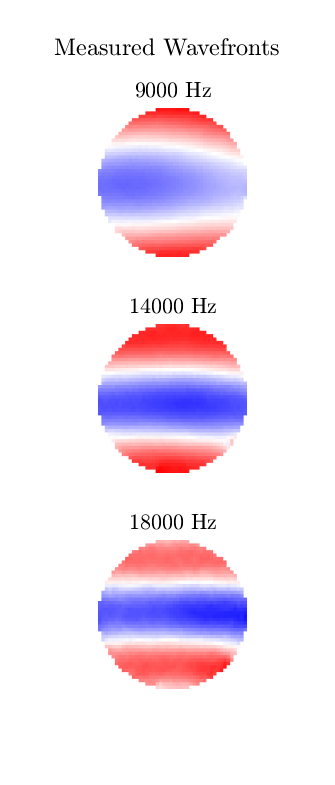
\includegraphics{../matlab/03_aero_optics_acoustics/spherical_plot_measured.eps}
  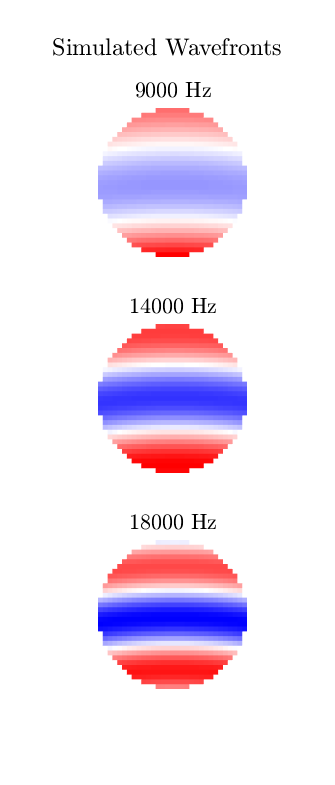
\includegraphics{../matlab/03_aero_optics_acoustics/spherical_plot_simulated.eps}
  \caption{Comparison of some of the measured wavefronts and simulated ones.}
  \label{fig:03_spherical_plot}
\end{figure}
The 9-kHz case shows some anomalies on the measured wavefront on the right side, diviating from spherical wave significantly likely contributing the significantly higher estimated pulsating field strength value when compared to the microphone estimate.
The 14 and 18-kHz cases show some remarkable agreement between the measured and simulated images.
Optical wavefront measurements can be utilized for making non-intrusive acoustic field measurements espically when the acoustic field is simple.



\section{Estimating the Acoustic Field Inside the Test-Section}



\subsection{Mode Marching Process}
\begin{enumerate}
  \item Start with a known or assumed source acoustic field, $p^n(x,y)$

  \item Calculate the transmitted pressure ratio
  \begin{itemize}
    \item Traveling with subsonic flow
      \begin{equation}
        \frac{p^t}{p^i} = \left(\frac{1+M_n}{1+M_{n+1}}\right)\left(\frac{2M_{n+1}}{M_n+M_{n+1}}\right)\left(\frac{X_{n,n}}{X_{n,n+1}}\right)\left(\frac{X_{n,n}}{X_{n+1,n+1}}\right)^{1/(\gamma-1)}
      \end{equation}
    \item Traveling against subsonic flow
      \begin{equation}
        \frac{p^t}{p^i} = \left(\frac{1-M_n}{1-M_{n+1}}\right)\left(\frac{2M_{n+1}}{M_n+M_{n+1}}\right)\left(\frac{X_{n,n}}{X_{n,n+1}}\right)\left(\frac{X_{n,n}}{X_{n+1,n+1}}\right)^{1/(\gamma-1)}
      \end{equation}
    \item Where
      \begin{equation}
        X_{a,b} = 1+\frac{\gamma-1}{2}M_aM_b
      \end{equation}
  \end{itemize}

  \item March acoustic field to next axial step,
    \begin{equation}
      p^{n+1}(x,y) = p^{n}(x,y)\frac{p^t}{p^i}\exp\{j(\omega t\mp k_{zm}^\pm z)\}
    \end{equation}

  \item Best-fit set of local duct modes coefficients, $C_m$, to acoustic field $p^{n+1}(x,y)$

  \item Calculate new acoustic field from duct mode and repeat from step 2
    \begin{equation}
      p^n(x,y) = \sum_{m=0}^{M} C_m\cdot p_m(x,y)
    \end{equation}

  \item When the end point is reached, step inlet acoustic field (rotate fan) and repeat
\end{enumerate}

    % !TEX root = catron-dissertation.tex
\epstopdfsetup{outdir=./images/04_dispersion_analysis/}

\chapter{Multidimensional Spectral Estimation of Optical Wavefronts}
\label{chap:04_dispersion}
% \begin{itemize}
%   \color{red}
%   \item
% \end{itemize}

As described in Chapter \ref{chap:01_intro}, the objective of this research is to develop methods to evaluate and, if possible, eliminate the effect of facility-related acoustic noise on aero-optical measurements.
As such, the first goal of the research is to establish analytical methods to identify and isolate acoustic sources of optical signals within a given data sample.
This is a significant challenge since, as will be shown later, acoustic sources of optical aberrations typically have a magnitude and frequency content that is in the same range as the signal that is the objective of the measurement.
This chapter will begin with a brief overview of some of the benefits to analyzing multidimensional data in this way, followed be a short discussion on how these spectra are calculated, and conclude with a more in depth discussion of the analysis of multidimensional spectral estimates.


The multi-dimensional spectral approach that is employed throughout this research helps identify and characterize acoustic sources of optical noise as well as aero-optical signals.
The spectral approach is also used as the basis for methods to filter the acoustic sources.
For measurements in multiple dimensions, such as a line of sensors that are recorded over time, a multidimensional spectral estimation not only produces temporal frequency content but can also be used to identify the direction and speed of travel of a particular wave.

The benefits of using multidimensional spectral estimation are shown in Figure \ref{fig:04_dispersion_demo}.
\begin{figure}
\centering
  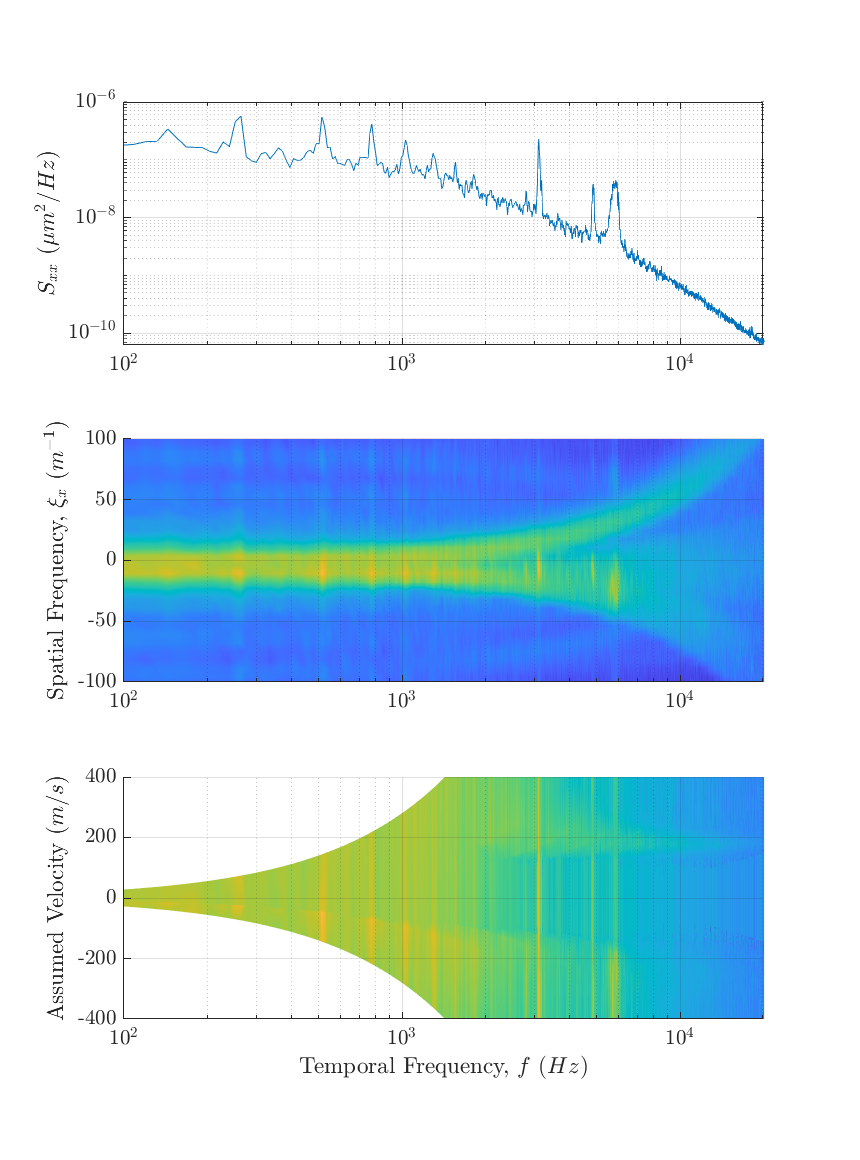
\includegraphics{../matlab/04_dispersion_analysis/dispersion_demo.eps}
  \caption{Multidimensional spectral estimation plot example and comparison to traditional power spectrum measurements. A single row of an optical wavefront measurement was used in this example. The top plot shows the typical power spectrum averaged over the entire row of data. Both the middle and bottom plots show the multidimensional spectrum plot with the y-axis as spatial frequency in the middle and velocity in the bottom assuming $u=f/\xi_x$.}
  \label{fig:04_dispersion_demo}
\end{figure}
The spectra shown in the figure were computed using the OPD measured by a single row of sub-apertures from a Shack-Hartmann optical wavefront measurement in which a 5 inch diameter beam was propagated normally through a wind-tunnel test section with a free-stream Mach number of 0.5.
This measurement was performed in the University of Notre Dame White Field Wind Tunnel in a test section that contained a model representing the fuselage of the AAOL aircraft \cite{Jumper-2013-8KtN3pue} with window that was flat and flush to the outer mold line of the fuselage.
The top plot shows a traditional power spectrum ensemble-averaged over the row of data.
Both the blade-passing frequency (517 Hz) and its sub-harmonic had similar amplitudes  with an additional five harmonics showing significant peaks.
There are three additional strong peaks at approximately 3100, 4850, and 5850 Hz that are likely due to fan vibration that limited the top speed of the tunnel for the test.

Both the middle and bottom plots show the multidimensional spectral estimation of the two-dimensional data, $\opd(x,t)$.
Since the figure is for illustrative purposes, colorbars were not shown; however, the color is representative of the logarithm of the power or variance in the wavefront signal (i.e. $\opdrms^2$) with yellow representing more power and blue representing less.
The colorbar range in this figure is the same for the middle and bottom plots and is consistent with the other plots throughout this chapter.
In the middle plot the y-axis represents the stream-wise spatial frequency, $\xi_x$ with the units of inverse meters.
It is important to note that, unlike temporal frequencies, spatial frequencies can have positive or negative values depending on the direction of travel of the disturbance,
in Figure \ref{fig:04_dispersion_demo}, waves with positive spatial frequencies are moving in the direction of flow.
In the middle plot of Figure \ref{fig:04_dispersion_demo}, there is a strong signal that roughly lies on the zero spatial frequency ($\xi_x\approx0$) axis up to a frequency of ~2000 Hz, after which the signal in the spectrum can be clearly seen to branch off into upstream- and downstream-moving disturbances.
The cause of the branching in the signal will be discussed later, however note that the reason why the signal appears to lie on $\xi_x\approx0$ at low frequencies is simply an artifact of plotting the spectrum on semilog axes (which was done to better resolve the peaks in the power spectrum in the top plot of the figure); as shown later in plots with linear axes, the signal actually branches off into upstream- and downstream-moving disturbances even at low frequencies.
The blade-passing frequency and its various harmonics can also be discerned in the center plot, by the vertical ``streaks'' that line up  with the peaks in the standard spectrum shown in the top plot; the center spectral plot shows that these fan blade-passing signals have significant broadband spatial frequency content.
All of these narrow-band signals have a majority of their signal traveling upstream.
In addition to optical disturbances branching off in the upstream and downstream moving directions there are significant disturbances along zero spatial frequency representing a collection of standing waves.
As already mentioned, he data in Figure \ref{fig:04_dispersion_demo} were plotted logarithmically along the temporal-frequency axis to better show the low frequency content around the fan blade-passing frequency, and how the peaks in the power spectrum in the top plot still appear in the multidimensional spectrum in the middle plot.
As shown later, when the multidimensional spectrum is plotted linearly, the two primary upstream and downstream traveling signals lay in a straight line.

A dispersion analysis can be performed on these multidimensional spectral estimates.
In order to obtain the velocity of a given wave we can start with the most basic forms of the wave equation,
\begin{equation}
  \hat{y} = a\exp\{j\theta\} \textrm{,}
\end{equation}
where $\theta$ is the phase of the wave and equal to $kx-\omega t$.
From here we can take the partial of $\theta$ with respect to time and set it equal to zero,
\begin{equation}
  \frac{\partial\theta}{\partial t} = 0 = \frac{\partial k}{\partial t}\frac{\partial x}{\partial t}-\frac{\partial \omega}{\partial t}\frac{\partial t}{\partial t} \textrm{,}
\end{equation}
which can be rearranged to
\begin{equation}
  u = \frac{\partial \omega}{\partial k} = \frac{\partial f}{\partial \xi} \textrm{.}
\end{equation}
If we are to assume that a wave packet intercepts the origin ($f=\xi=0$) then every point on the spectral plot can be assumed to have a disturbance velocity,
\begin{equation}
  u_{d} = \frac{f}{\xi_x} \textrm{.}
  \label{eqn:04_velocity_assumed}
\end{equation}
This relationship shows that, for a nondispersive medium such as air, the spatial frequency of a disturbance is related linearly to the temporal frequency as $1/u_d$.
The bottom plot shows the same multidimensional spectral estimation plot as the middle one but with the y-axis showing disturbance velocity $u_d$.
The bottom plot shows that the primary optical disturbance moving in the direction of flow is moving at the free-stream velocity of approximately 175 m/s.
The upstream traveling disturbance is traveling at the same speed but due to the signal being broader is more difficult to measure this way.
Note that the stationary modes along $\xi_x\approx0$ in the middle plot are nowhere to be found on the bottom plot; this is because when the disturbance velocity for this these waves is calculated their speed approaches infinity.

\section{One-Dimensional Power Spectrum Calculation}
Power spectral analysis is typically performed on one-dimensional data sets, for example, a single sensor measurement over time.
On the other hand, as shown in Figure \ref{fig:04_dispersion_demo}, if a sensor array were used, a multi-dimensional power spectrum could be computed that would also show spatial frequency information.
For a single-point measurement that varies in time, $x(t)$, the power spectrum calculation is
\begin{equation}
 S_{xx} = \frac{|\fft\{x(t)\}|^2}{Nf_{s}} \textrm{,}
 \label{eqn:04_basic_sxx}
\end{equation}
where $\fft$ is the Fast Fourier Transform, $N$ is the number of samples, and $f_{s}$ is the sample rate \cite{Blackman-1958-4QtKgDb8}.
For data that has only a real component the Fast Fourier Transform function produces magnitude and phase relations at each frequency step, $f_{s}/N$, over the range from zero-frequency up to but not including the Nyquist frequency, $f_s/w$, with a mirrored set of data that can be represented either below (starting at $-f_s/2$) or above (ending just below $f_s$) this range.
The Nyquist frequency not being included and the mirrored data is due to an assumption that is integral to the Fourier Transform, which is that the signal is assumed to be periodic.

The total energy, $\sigma^2$, of the signal must be preserved through the transform from physical space-time to frequency space
\begin{equation}
  \sigma^2 = \frac{\sum x^2(t)}{N} = \Delta f\sum S_{xx}(f) \textrm{.}
  \label{eqn:04_fft_energy_conservation}
\end{equation}
Additionally, because of the periodic nature of the Fourier Transform and a finite sample length of discrete data, spectral leakage can cause the power in one frequency bin to leak into adjacent frequency bins.
To minimize this spectral leakage, windowing functions are employed which typically force the end points of the signal to zero.
The Hann window,
\begin{equation}
 w(t) = 1/2\left[1-\cos\left(\frac{2\pi t}{T}\right)\right] \textrm{,}
 \label{eqn:04_hann_window}
\end{equation}
is one of the more commonly used windowing functions \cite{Braun-2001-qhqBfvYz} where $w(t)$ is the window function, $t$ is the time at a given sample, and $T$ is the total sample time.
Since the windowing of a data set changes the signal energy some correction is needed to be applied.
For an arbitrary windowing function the correction factor, $c_w$, can be obtained by substituting the windowing function in place of $x(t)$ in Equation \ref{eqn:04_fft_energy_conservation},
\begin{equation}
 c_w = \frac{1}{\sqrt{\sum w^2(t)/N}} \textrm{.}
 \label{eqn:04_window_correction}
\end{equation}
For a Hann window this correction factor approaches $\sqrt{8/3}$ as $N$ goes to infinity.
When Equation \ref{eqn:04_basic_sxx} is combined with a windowing function and associated correction the double sided power spectra equation in one dimension becomes
\begin{equation}
 S_{xx} = \frac{|c_w\fft\{x(t) w(t)\}|^2}{Nf_{s}} \textrm{.}
 \label{eqn:04_windowed_sxx}
\end{equation}

\section{N-Dimensional Power Spectra Calculation}
For measurements with multiple spatial and temporal dimensions the Fast Fourier Transform is applied $n$-times where $n$ is the total number of dimensions, with each application in a different dimension,
\begin{equation}
 \fftn(x) = \fft(\fft(\cdots\fft(\fft(x,1),2)\cdots,n-1),n) \textrm{,}
 \label{eqn:04_fftn}
\end{equation}
where $\fft(x,n)$ is the Fast Fourier Transform of $x$ in the $n^{th}$ dimension \cite{An-1991-QKg7heKm}.
For a $n$-dimensional array the operation becomes \cite{McClellan-1982-rGQzuZ7t}
\begin{equation}
 \mathbf{S_{xx}} =\frac{|c_w\fftn\{f(\mathbf{x}) w(\mathbf{x})\}|^2}{\prod{\overrightarrow{N}\overrightarrow{f_s}}} \textrm{,}
 \label{eqn:04_sxxn}
\end{equation}
where $\mathbf{S_{xx}}$ is the $n$-dimensional power spectra array or dispersion array, $f(\mathbf{x})$ is an $n$-dimensional set of data, $w(\mathbf{x})$ is an $n$-dimensional windowing function, $\overrightarrow{N}$ is a vector denoting the number of elements in each dimension, $\overrightarrow{f_s}$ is a vector denoting the sample rate in each dimension, and
\begin{equation}
 c_w = \frac{1}{\sqrt{\sum w^2(\mathbf{x})/\prod{\overrightarrow{N}}}} \textrm{.}
 \label{eqn:04_windown}
\end{equation}
The signal energy conservation relationship becomes
\begin{equation}
  \sigma^2=\frac{\sum\mathbf{x}}{\prod{\overrightarrow{N}}} = \prod{\overrightarrow{\Delta f_s}}\sum\mathbf{S_{xx}} \textrm{,}
  \label{eqn:04_fftn_energy_conservation}
\end{equation}
where $\overrightarrow{\Delta f_s}$ is a vector representing the frequency step sizes in each dimension.

\section{Non-Rectangular Spatial Windows}
For n-dimensional data sets that fill a rectangular array, a windowing function can be created by multiplying together a series of one-dimensional windowing functions in the direction of each dimension.
For non-rectangular data sets, such as is often the case with optical wavefront measurements, a windowing function can take some additional steps in its construction.
In cases when the spatial measurement locations are constant throughout time, the windowing function can be split into two separate components,
\begin{equation}
 w(\mathbf{x}) = w_t(t)\cdot w_s(x,y) \textrm{,}
 \label{eqn:04_window_sep}
\end{equation}
the temporal windowing function, $w_t(t)$, and the spatial windowing function, $w_s(x,y)$.
This study uses a Hann window for the temporal windowing function and a modified Hann window for the spatial windowing function.
For the case of a perfectly circular aperture, the Hann window can be reformulated to be based on the normalized radius, $\rho_N$, of the aperture,
\begin{equation}
 w_s(\rho_N) =
 \begin{cases}
  \frac{1+\cos(\pi\cdot\rho_N)}{2} & \textrm{if } \rho_N < 1 \\
  0                                & \textrm{otherwise.}
 \end{cases}
 \label{eqn:04_window_space}
\end{equation}
This modified Hann window is two-dimensional with a value of one at the center of the aperture and decreases to zero at the edge of the aperture in the same manner as a Hann windows decreases from the center to either end.

Because the wavefronts measurements often had a clipped edge or some other obscuration, a different method was employed in this study.
For an arbitrary shaped aperture, the minimum distance from any given measurement location to the edge of the aperture was used to create the spatial windows.
The minimum distance can be computed given the a set of points ($x$ and $y$) that spans the measurement range and the set of points outside of the aperture ($x_O$ and $y_O$),
\begin{equation}
 d_{min}(x,y) = \min\left\{\sqrt{(x-x_{O})^2+(y-y_{O})^2}\right\} \textrm{.}
 \label{eqn:04_window_space_arb_dist}
\end{equation}
This distance is then normalized by the maximum value and the resulting spatial window given a modified Hann window,
\begin{equation}
 w_s(x,y) = \frac{1+\cos\left\{\pi\cdot\left(1-d_{min}^{norm}(x,y)\right)\right\}}{2} \textrm{.}
 \label{eqn:04_window_space_arb}
\end{equation}
% An arbitrary aperture and its corresponding spatial window are shown in Figure \ref{fig:04_spatial_window}.
% \begin{figure}
%   \centering
%   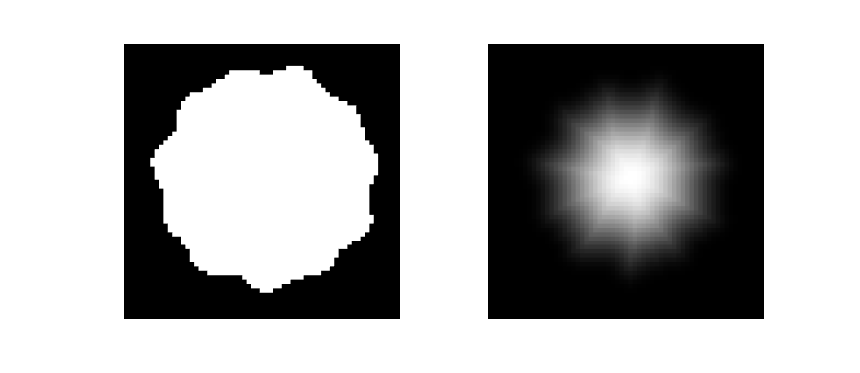
\includegraphics{../matlab/04_dispersion_analysis/spatial_window.eps}
%   \caption{An arbitrary nearly round aperture and its corresponding spatial window.}
%   \label{fig:04_spatial_window}
% \end{figure}
% This aperture is nearly circular with slight perturbations along the edge.
This same basic idea can be extended to data sets where the locations of measurements in space vary with time.

\section{Wavefront Multidimensional Spectrum}
At the beginning of this chapter a multidimensional spectral plot for data resolved in time and one spatial dimension was shown along with a typical power spectrum plot in Figure \ref{fig:04_dispersion_demo}.
This was shown to facilitate a simple discussion of some of the benefits of using multidimensional spectrum analysis on optical wavefronts.
That simple analysis was performed on only a single row of a wavefront data set and provided an insight into the disturbances that were moving in the horizontal (stream wise) direction only.
When multidimensional spectral estimation is performed over all dimensions of a wavefront (i.e. time and both spatial dimensions), as will be done for the remainder of this chapter, additional detail is available, that also enables the determination of optical disturbances moving vertically (i.e. cross-stream to the flow) or in any direction in between.
Figure \ref{fig:04_dispersion_comparison} shows a comparison between the two-dimensional single row spectrum (bottom plot) with two different representations of the same two-dimensional spectrum extracted from a three-dimensional spectral calculation.
\begin{figure}
  \centering
  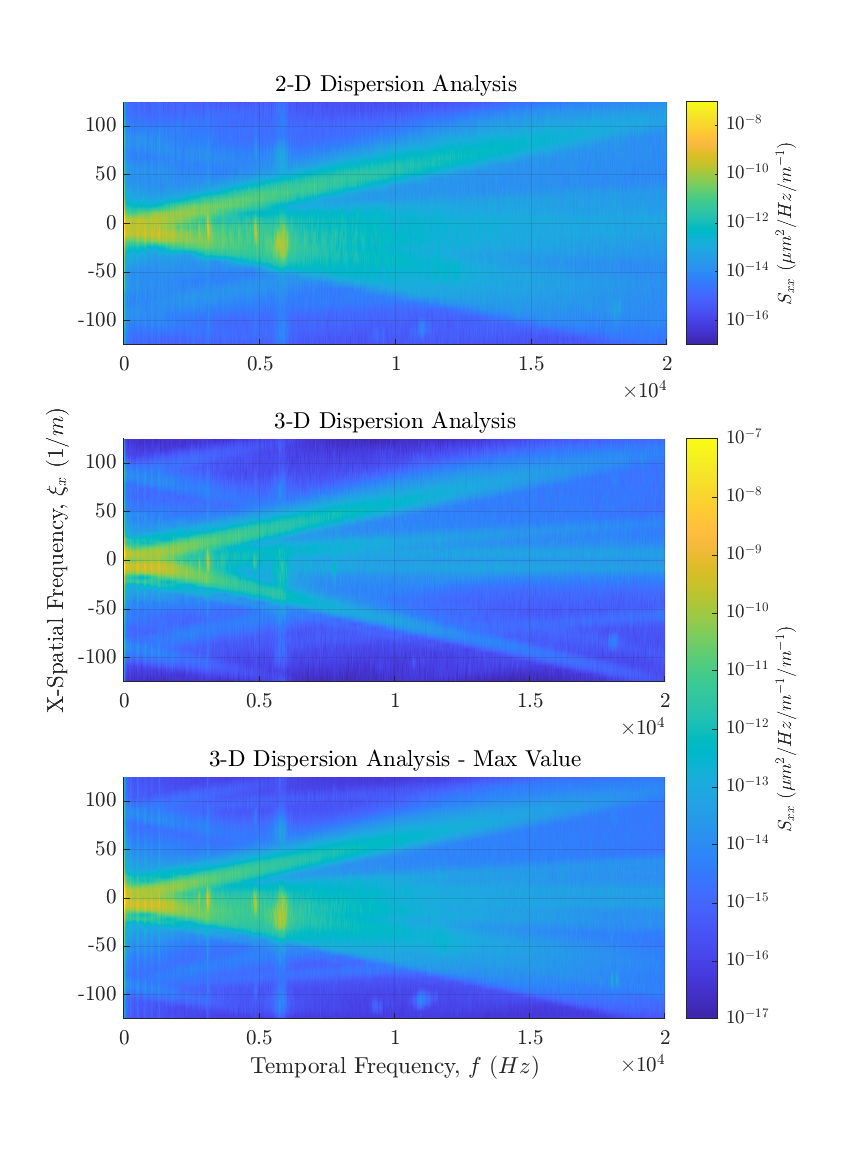
\includegraphics{../matlab/04_dispersion_analysis/dispersion_comparison.eps}
  \caption{Horizontal moving optical disturbances comparison. The top plot shows a slice of the three-dimensional spectrum focusing on the plane waves that are traveling in the horizontal direction. The middle plot is a recreation of the two-dimensional spectrum by integrating through the the vertical spatial frequencies. The bottom plot is the two-dimensional spectrum.}
  \label{fig:04_dispersion_comparison}
\end{figure}
Specifically, the top plot in Figure \ref{fig:04_dispersion_comparison} shows the ``slice'' of the three-dimensional spectral estimation plot taken at $\xi_y=0\ m^{-1}$; because this slice does not contain any information on vertically-moving disturbance, it shows planar waves traveling in the horizontal direction.
The middle plot shows the same three-dimensional spectrum integrated through the vertical spatial frequency axis to create an estimate of the two-dimensional spectrum.
The bottom plots shows the two-dimensional spectral plot that was previously shown in Figure \ref{fig:04_dispersion_demo} but this time with a linear temporal frequency axis.
Both of the two-dimensional spectra in the top two plots of Figure \ref{fig:04_dispersion_comparison}, whether directly computed or integrated show a significant increase in the signal content between the acoustic lines ($u\pm c$).

The three-dimensional spectral slice (top plot) shows significant signal energy at the same characteristic velocities of the free-stream velocity, $u$, and the acoustic lines, $u\pm c$, as the two-dimensional spectrum (bottom plot), along with some additional signal laying along the temporal-frequency axis at $\xi_y=0\ m^{-1}$.
This signal represents a collection of stationary modes at each temporal frequency.
If this were a flow-related phenomenon the velocity of the disturbance according to Equation \ref{eqn:04_velocity_assumed} would be near infinity; as such, it is more likely caused by mechanical vibration of the wind tunnel and components of the optical measurement system.
On the three-dimensional spectrum plot there are signals that run parallel to $u$ and $u-c$ that do not emanate from the origin but from $\xi_x\approx\pm80\ m^{-1}$; at present an explanation for these signals cannot be given; however, it is possible that this effect is caused by an optical ghost image.
There is also an aliased signal that runs parallel to $u+c$ starting on the right side of Figure \ref{fig:04_dispersion_comparison} top at $\xi_x\approx-50\ m^{-1}$ and decaying towards the left.
Aliased signals are due to the sample rate, either spatial or temporal, being to low.

The middle plot of Figure \ref{fig:04_dispersion_comparison} shows the integrated spectrum through the vertical spatial frequency axis.
This integration captures the energy in all vertical disturbances which effectively recreates the two-dimensional spectrum plot on the bottom of Figure \ref{fig:04_dispersion_comparison}.
A reduced order spectrum like this is calculated by
\begin{equation}
  S_{xx}^{n-1} = \int S_{xx}^n df_s^m \textrm{,}
\end{equation}
where $S_{xx}^n$ is the n-dimensional spectrum and $df_s^m$ is the differential frequency in the $m$-th dimension.
This is also shown in Figure \ref{fig:04_dispersion_max}.
\begin{figure}
  \centering
  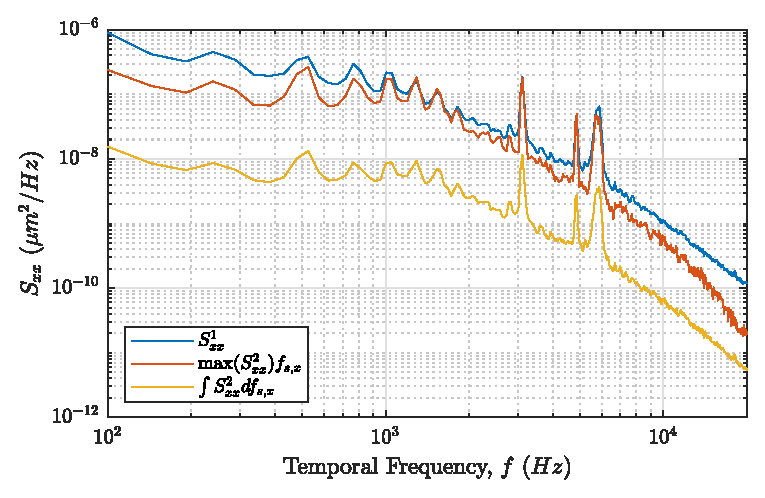
\includegraphics{../matlab/04_dispersion_analysis/dispersion_max.eps}
  \caption{Recovery of time-based power spectrum from two-dimensional spectral estimate.}
  \label{fig:04_dispersion_max}
\end{figure}
While the integrated signal over estimated the spectrum going from three-dimensions to two in Figure \ref{fig:04_dispersion_comparison}, it under estimates the spectrum going from two to one dimensions.
Unfortunately, due to the limited number of spatial sample points and the large dynamic range of the signal, this integrated value can contain a significant amount of error.

Due to the the signal containing a majority of the power in a limited number of spatial frequency bins, a reduced order spectrum can be estimated by
\begin{equation}
  S_{xx}^{n-1} \approx \max(S_{xx}^n,m)f_s^m \textrm{,}
\end{equation}
where $\max(S_{xx}^n,m)$ is the maximum value of the spectrum along dimension $m$ and $f_s^m$ is the sample rate for that dimension.
The calculated temporal power spectrum from the two-dimensional spectrum using the maximum value is a good estimation at the center of the frequency range but has some additional decay at both low and high frequencies.
The calculated reduced order spectrum in Figure \ref{fig:04_dispersion_max} (red curve) appears to follow the functional form of the actual one-dimensional spectrum (blue curve) but with a small offset.

\subsection{2-D Slices of the Multidimensional Spectral Estimation}
The full multidimensional spectrum contains information of flow features that are not only moving in the horizontal (stream-wise) direction as the two-dimensional dispersion showed but also in every direction of the two-dimensional optical wavefront.
Figure \ref{fig:04_dispersion_xy} shows two-dimensional slices of the full spectrum that on the top show the horizontal (stream-wise) moving disturbances for a vertical spatial frequency of $\xi_y=0$ $m^{-1}$ and on the bottom show the vertical (cross-stream) moving disturbances for a horizontal spatial frequency of $\xi_x=0$ $m^{-1}$.
\begin{figure}
  \centering
  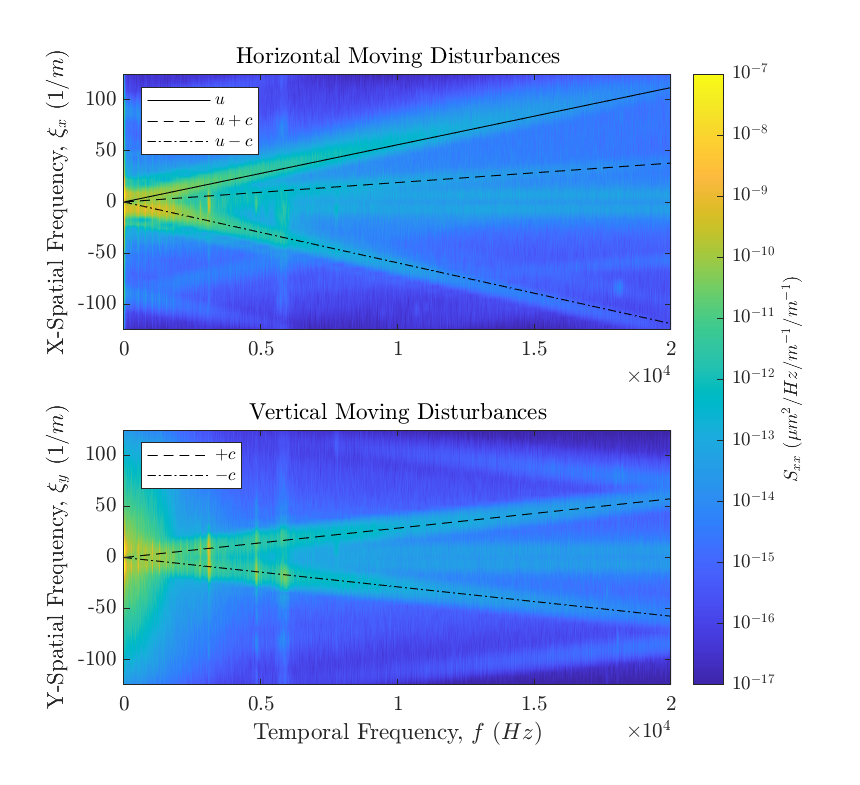
\includegraphics{../matlab/04_dispersion_analysis/dispersion_xy.eps}
  \caption{Horizontal and vertical moving optical disturbances. This is the same data as presented in Figure \ref{fig:04_dispersion_demo} but after calculating the full three-dimensional spectral estimate. These optical disturbances are plane waves that are traveling solely in their respective directions.}
  \label{fig:04_dispersion_xy}
\end{figure}
Since the wavelength is $\lambda=1/\xi$, the waves that make up the disturbances shown in these slices are plane waves that are traveling solely in the horizontal or vertical directions.

The top plot of Figure \ref{fig:04_dispersion_xy} shows the two-dimensional spectrum for horizontally moving optical disturbances that was shown previously.
There are three major flow-related structures that can be observed.
The large signal that lays along $u$ (solid line in Figure \ref{fig:04_dispersion_xy}) is the aero-optical effect of the boundary layers on both walls of the wind tunnel.
It can be seen that the boundary-layer signal has a peak slightly less than the free-stream velocity, $u$, and has a slight decay as the velocity decreases away from the peak and a sharp decay as the velocity increases.
For reference, the dotted line at the top of Figure \ref{fig:04_dispersion_xy} denotes a velocity of $0.7u$.
The velocity of the strongest aberrating structures in the boundary layer has typically been reported as approximately 0.83$u$ \cite{Gordeyev-2014-jcJndkHM}, however, this data shows the boundary layer velocity has a range of velocities at each given frequency in which the peak velocity component has some dependence on the temporal frequency.
This can be more clearly seen in two temporal frequency slices in Figure \ref{fig:04_dispersion_slices_velocity} which shows vertical spatial frequency plotted against the normalized horizontal (stream-wise) velocity.
\begin{figure}
  \centering
  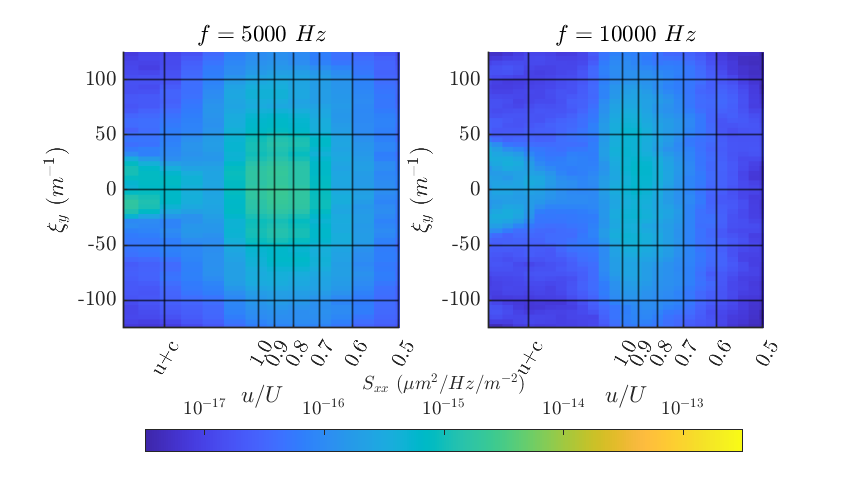
\includegraphics{../matlab/04_dispersion_analysis/dispersion_slices_velocity.eps}
  \caption{Temporal-frequency slices at 5 and 10 kHz with the various horizontal velocities labeled.}
  \label{fig:04_dispersion_slices_velocity}
\end{figure}
Again, the figure shows strong decay of the signal as the speed increases above the free-stream velocity and gradual decay as the speed decreases.
There is also additional signal decay as the absolute value of the vertical spatial frequency increases.
The velocity of this boundary layer optical disturbance will be measured in Chapter \ref{chap:06_single_filter} using a velocity filter to show a mean velocity of $0.85u$, which is near the generally accepted value of $0.83u$ \cite{Gordeyev-2014-jcJndkHM}.

The other two major flow-related structures in Figure \ref{fig:04_dispersion_xy} are related to acoustic signals traveling in both directions through the wind-tunnel, denoted by the dashed and dot-dash lines in the figure.
The downstream-traveling acoustic wave, $u+c$, has a low signal power than the upstream-traveling acoustic wave, $u-c$.
The likely explanation for this difference in signal power is that most of the acoustic energy in the wind tunnel is generated by the fan which propagates upstream and downstream within the wind-tunnel ducting.
However, sound waves that move in the flow direction have their wavelength stretched as the flow is accelerated into the test-section contraction, while sound waves moving against the flow have their wavelength contracted.
Hence the downstream-traveling waves have a longer wavelength as they pass through the measurement beam and thus more of the optical signal from the downstream-travelling waves is filtered out due to aperture filtering \cite{Siegenthaler-2008-9Yutbt6c}.
At low temporal frequencies, the blade-passing frequency (~520 Hz) and its associated harmonics appear as vertical lines with regular spacing in Figure \ref{fig:04_dispersion_xy}.
% There also appears to be some constructive interference with the BPF and some of the aliased data around $\xi_x = \pm100\ m^{-1}$.

The two main features on the vertical spectral slice plot on the bottom of Figure \ref{fig:04_dispersion_xy} are the signals moving at the speed of sound ($\pm c$) including some significant aliasing of these signals.
These two lines represent acoustic waves that are traveling either straight up or down through the measurement beam.
The blade-passing frequency and its harmonics are also visible in the vertical moving wave plots in both directions and have much less broadband spatial content in the vertical direction.
There are also high temporal frequency narrow-band signals ($\sim$3, 5, and 6 kHz) that contain most of their signal power at the speed of sound lines.
These signals have some dependence on the free-stream Mach number (see Figure \ref{fig:04_dispersion_mach}).
These maybe vibrations originating from the tunnel fan that are currently limiting the top speed of the tunnel; some older optical wavefronts collected in this tunnel under similar measurement conditions do not show these narrow-band signals.
Because the portion of these signals with the most power is traveling vertically through the test section instead of steam wise, the tunnel walls maybe excited by the fan and resonating.

The stationary modes that have been discussed previously that appear as a broad horizontal band along the temporal frequency axis in the horizontal spectral slice plot also appear in the same location in the vertical spectral slice plot.
These stationary modes appear the be constant when viewed from either direction and through out time.
As stated by Blackman and Tukey, this kind of white-noise is generally not physical unless it is bandwidth limited with a falloff of at least $1/f^2$ \cite{Blackman-1958-4QtKgDb8}.
Some of these stationary modes are likely cause by vibrations of various optical elements, especially at low temporal frequencies.
At higher temporal frequencies, the stationary modes maybe related to electronic noise from the high-speed camera, higher order optical noise from the laser, or even numerical error from the processing code.

\subsection{3-D Representations of Multidimensional Spectral Estimation}
While the two-dimensional slices are fairly informative, particularly when it comes to signal strength of various flow structures and their velocities, a three-dimensional plot allows better visualization of the overall flow structures although some details are lost because typically only one power level can be plotted at a time.
The same data that has been previously shown in two-dimensional form, is depicted in Figure \ref{fig:04_dispersion_isosurface} as an isosurface with a power of $10^{-14}$ $\mu m^2/Hz/m^{-2}$ and shown from four different views in Figure \ref{fig:04_dispersion_3d}.
\begin{figure}
  \centering
  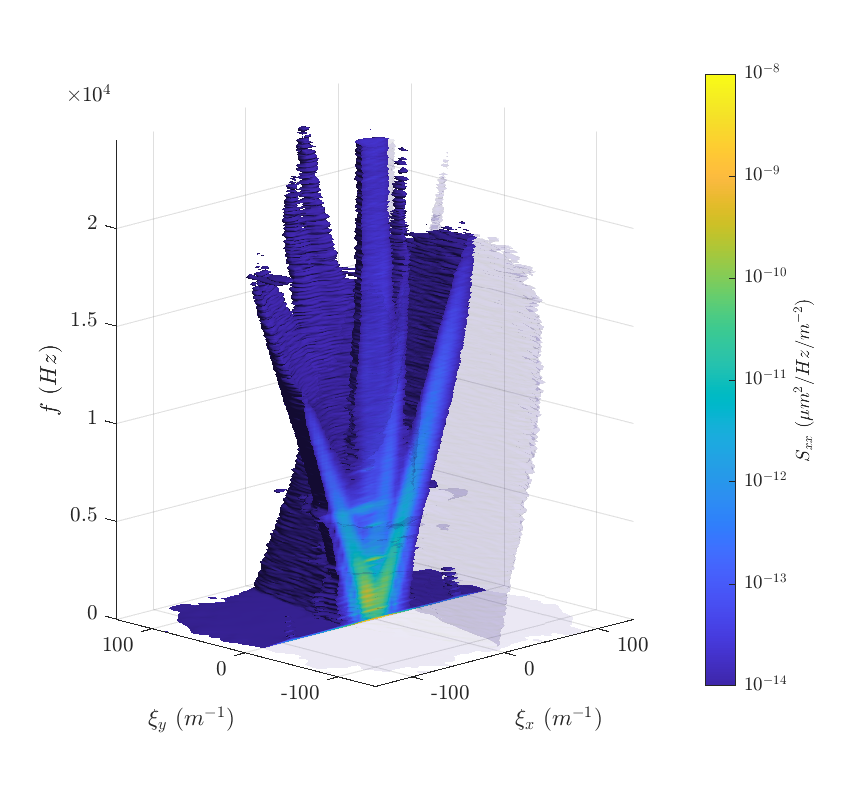
\includegraphics{../matlab/08_conclusion/dispersion_isosurface.eps}
  \put(-195,120){\rotatebox{76}{\Large Boundary Layer}}
  \put(-305,250){\rotatebox{-75}{\Large Acoustic Cone}}
  \put(-300,69){\textcolor{white}{\Large BPF $\Longrightarrow$}}
  \put(-231,180){\textcolor{white}{\rotatebox{90}{\Large Stationary Modes}}}
  \put(-235,50){\rotatebox{15}{\Large Mean-Lensing}}
  \caption{Multidimensional spectral estimation of an optical wavefront measurement made in a wind tunnel.}
  \label{fig:04_dispersion_isosurface}
\end{figure}
\begin{figure}
  \centering
  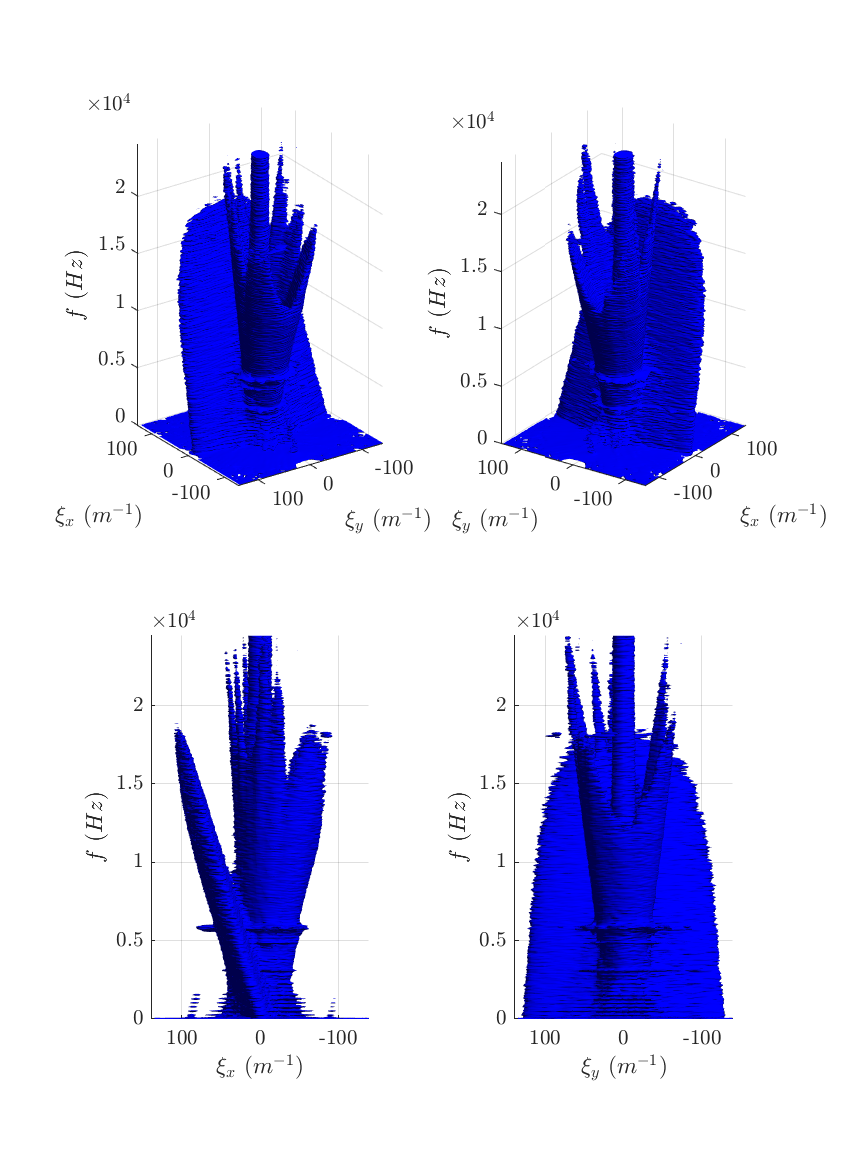
\includegraphics{../matlab/04_dispersion_analysis/dispersion_3d.eps}
  \caption{Three-dimensional view of the multidimensional spectral plot showing an isosurface at a power of $10^{-14}$ $\mu m^2/Hz/m^{-2}$.}
  \label{fig:04_dispersion_3d}
\end{figure}
The largest feature is the boundary layer signal which resembles an ellipsoidal plane that is tilted in the $f-\xi_s$ plane.
The other main feature is the acoustic signal which appears as a cone which is slightly tilted in the direction of upstream-moving disturbances.
The acoustic signal separates into several spikes at high temporal frequencies some of which are constructive interference from aliased signal ($\xi_x\approx25\ m^{-1},\ \xi_y\approx\pm60\ m^{-1}, \textrm{and}\ f\approx20 kHz$) which is better visualized in the 20 kHz temporal frequency spectral slice in Figure \ref{fig:04_dispersion_slices_velocity}.
There may also be a small number of dominant duct modes at these high temporal frequencies.
The last feature is the stationary modes which appears as the cylindrical structure along the center of the plot (near zero spatial frequency in x and y), which have a near constant shape and magnitude through all temporal frequency ranges.

Figure \ref{fig:04_dispersion_mach} shows two views of an isosurface of the multidimensional spectrum over a range of Mach numbers.
\begin{figure}
  \centering
  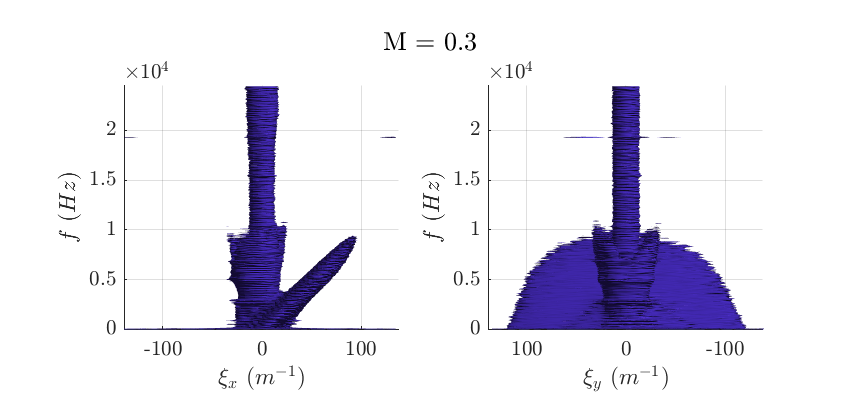
\includegraphics{../matlab/04_dispersion_analysis/dispersion_mach_0.3.eps}
  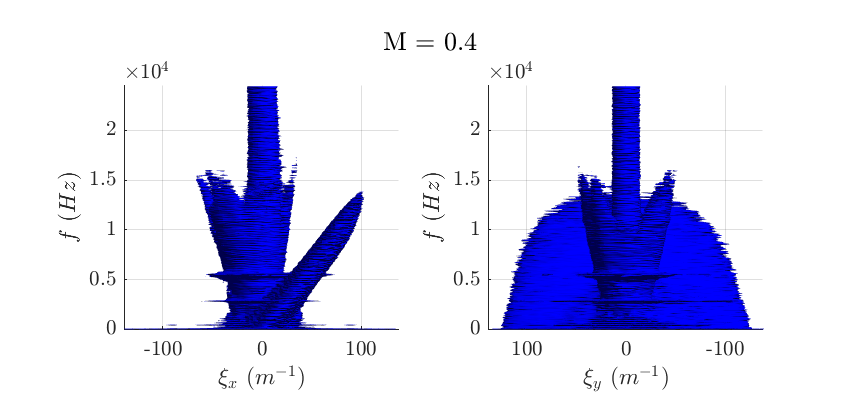
\includegraphics{../matlab/04_dispersion_analysis/dispersion_mach_0.4.eps}
  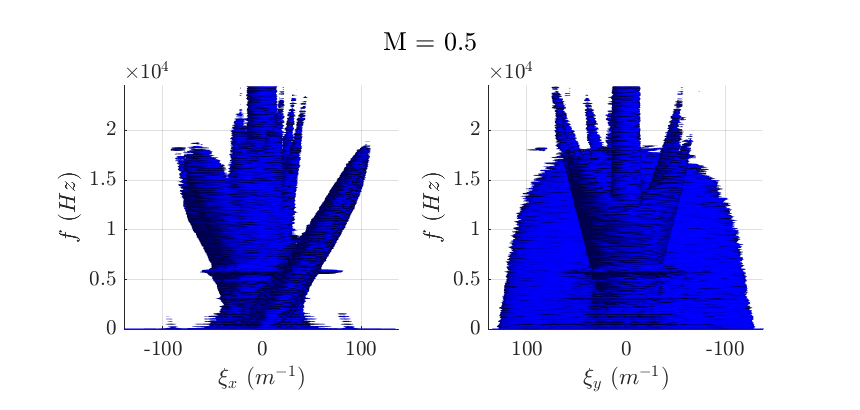
\includegraphics{../matlab/04_dispersion_analysis/dispersion_mach_0.5.eps}
  \caption{Multidimensional spectral estimate isosurfaces as the Mach number increased from 0.3 to 0.5. The isosurfaces are all shown at a power of $10^{-14}$ $\mu m^2/Hz/m^{-2}$.}
  \label{fig:04_dispersion_mach}
\end{figure}
All of these plots are of an isosurface with the same power as used in Figure \ref{fig:04_dispersion_3d}.
The stationary modes seem to be constant throughout the range of Mach numbers indicating that they are most likely not flow related.
The boundary layer signal increases in power significantly as the Mach number is increased while also the slope and thus the velocity is significantly increased as well.
As shown in  and discussed in Chapter \ref{chap:02_lit_review}, the aero-optical $\opdrms$ of the flat-plate boundary layer on the walls of the wind tunnel is expected to vary according to Equation \ref{eqn:02_opdrms_gor}.
Hence the significant increase in the power of the boundary-layer spectrum with Mach number that can be observed in Figure \ref{fig:04_dispersion_mach} is expected based on the $M^2$ dependence in Equation \ref{eqn:02_opdrms_gor}.
The increase in slope of the boundary-layer signal is also expected, and is caused by the increase in the convection speed of the boundary-layer aero-optical disturbances as the free-stream Mach number increases.
The acoustic signal sees some interesting evolution as well.
Along with the strength greatly increasing with Mach number, the slope of the upstream traveling disturbances decreases significantly while the downstream moving acoustic disturbances do not see much change other than an increase in signal strength.

As the angle of the optical beam changes as it passes through the test section the horizontal spatial frequency goes from measuring only the axial component of the optical disturbance to measuring a combination of the axial and span-wise component.
This can be seen in Figure \ref{fig:04_dispersion_angle} with the same isosurface value as shown in previous figures and at a Mach number of 0.5.
\begin{figure}
  \centering
  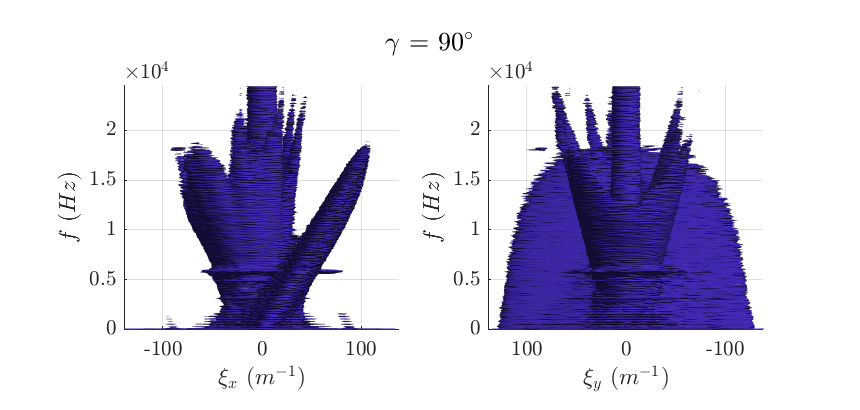
\includegraphics{../matlab/04_dispersion_analysis/dispersion_angle_90.eps}
  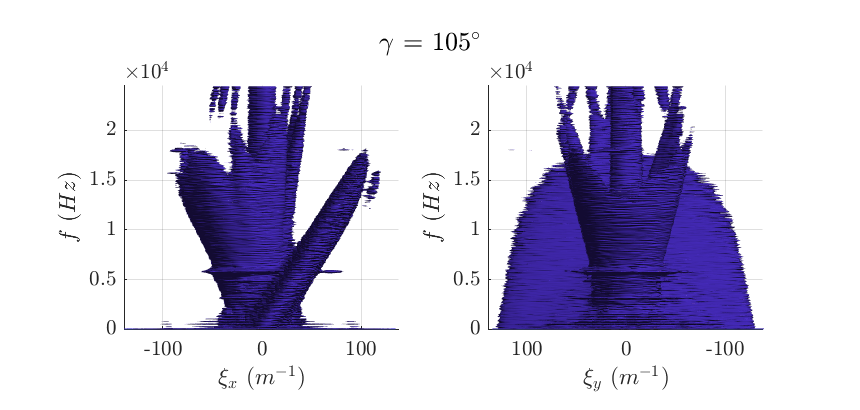
\includegraphics{../matlab/04_dispersion_analysis/dispersion_angle_105.eps}
  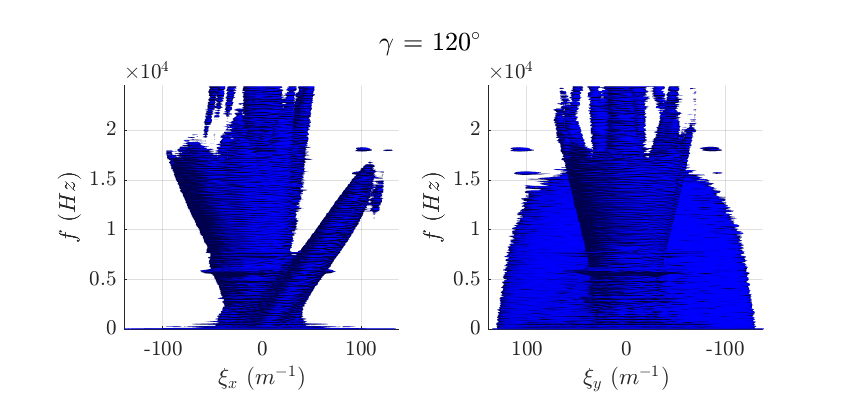
\includegraphics{../matlab/04_dispersion_analysis/dispersion_angle_120.eps}
  \caption{Multidimensional spectral estimate isosurfaces of different viewing angles through the test section at a Mach number of 0.5. The isosurfaces are all shown at a power of $10^{-14}$ $\mu m^2/Hz/m^{-2}$.}
  \label{fig:04_dispersion_angle}
\end{figure}
The $90^\circ$ beam case at the top of Figure \ref{fig:04_dispersion_angle} has been shown previously and the vertical component of the optical  disturbance sees little change as the viewing angle is increase except a small reduction in the boundary layer signal and some additional signal at the high temporal frequencies in the acoustic cone.
As the angle is increased the side of the acoustic cone traveling in the direction of flow is significantly increased in power, with a large amount of the signal being aliased into the upstream-traveling side appearing as `stalactites' at odd angles.
The upstream-traveling acoustic signal is also increased in power but to a lesser extent.
The stationary mode pillar experiences some change as well as the viewing angle hits $120^\circ$ and is stretched in the horizontal direction.As the beam angle increases, the acoustic duct modes begin to overlap one another in spectral space causing significant constructive interference.
This will be shown and discussed more fully later in Section \ref{sect:04_acoustic_cone}.
The effective velocity of the optical disturbances is reduced for the disturbances traveling in the same direction as the flow and increased for the disturbances traveling in the opposite direction.


While these three-dimensional isosurfaces offer some significant insight into the overall structure of the various optical disturbances they do not fully show the spectral details.
Plots of spatial vs temporal frequencies for the horizontal and vertical plane waves were shown in Figure \ref{fig:04_dispersion_xy} while Figure \ref{fig:04_dispersion_slices} shows slices at various temporal frequencies.
\begin{figure}
  \centering
  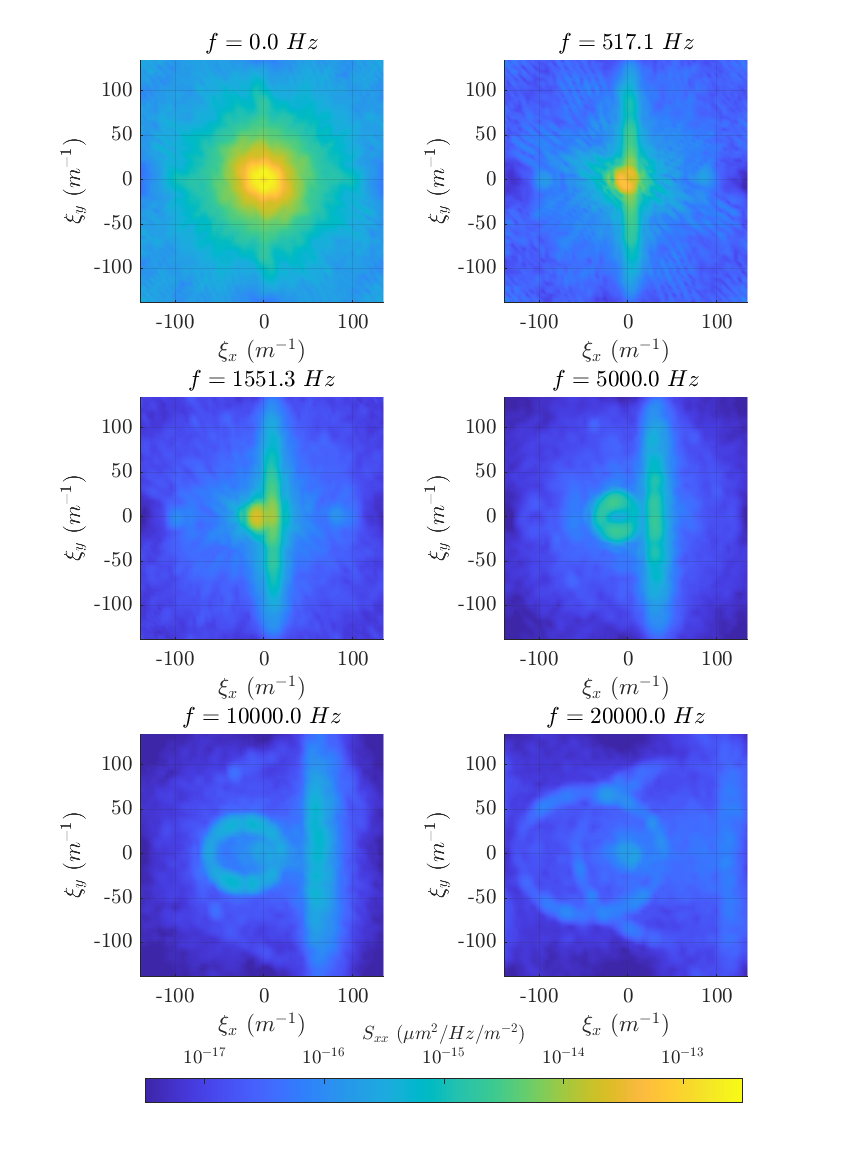
\includegraphics{../matlab/04_dispersion_analysis/dispersion_slices.eps}
  \caption{Multidimensional spectral estimate slices at various temporal frequencies.}
  \label{fig:04_dispersion_slices}
\end{figure}
The temporal frequencies spectral slices shown are at: 0 Hz, the blade-passing frequency at 517 Hz, the second harmonic of the blade-passing frequency at 1551 Hz, and additional slices at 5, 10, and 20 kHz.
The slice at 0 Hz temporal frequency shows the spatial frequencies of the wavefront disturbance that does not change with time.
This temporally constant wavefront disturbance is typically called the ``mean lensing''component of the wavefront measurement, since it is has an effect similar to a lens placed in the beam.
The mean lensing slice at 0 Hz shows a mostly axisymmetric pattern with most of its power concentrated at low spatial frequencies.
There appear to be the occasional spike radiating out from the center, most noticeably in line with the boundary layer signal.

The next four slices, for $f$=517.1 Hz to 10 kHz, show a vertical line associated with the boundary layers aero-optical disturbance, which  progressively moves towards positive x-spatial frequencies with increasing frequency.
The boundary-layer disturbance appears to be rotated slightly counter-clockwise indicating that the interrogation beam is slightly rotated between the test section and the wavefront sensor.
The boundary layer signals at the lower temporal frequencies appear to have equal decay in both the positive and negative $\xi_x$ directions while at the higher frequencies, the decay is much more gradual in the positive $\xi_x$ direction.
This could be indicative of the lower temporal frequency disturbances in the boundary layer typically traveling at a more uniform speed very near the free-stream velocity likely being either in the outer boundary layer or free-stream tunnel turbulence.
The higher temporal frequency disturbances seem to have a much wider range of velocities that approach the free-stream velocity and are likely small structures that reside in different parts of the boundary layer and hence travel with a wide range of convection velocities.

The acoustic disturbances show an interesting evolution as the temporal frequency increases.
At low temporal frequencies, the acoustic disturbances are concentrated near zero spatial frequency and with strong power.
At high temporal frequencies the acoustic disturbances appear as elliptically shaped rings.
At 20 kHz, there are two elliptical shapes that are easily identifiable, the smaller one is the signal that is actually present at that frequency while the other one is aliased data due to the limited temporal sample rate.
There is constructive interference where the two acoustic rings intersect.
The 10 kHz slice also shows a small amount of acoustic aliasing
Both the 10 and 20 kHz acoustic rings show some a non-uniform signal power throughout the circumference which are also visible in the three-dimensional views as the spikes at the high temporal frequencies.

\subsection{Acoustic Cone}
\label{sect:04_acoustic_cone}
The shape of the acoustic cone can be visualized by plotting the relationship between the temporal frequency and the vertical (i.e. cross-stream) and axial (i.e. stream-wise) wavenumbers for a series of acoustic duct modes .
Figure \ref{fig:04_dispersion_sound} shows the acoustic cone mode lines for a small set of duct modes at various Mach numbers for a duct that is 1 meter square and a beam passing through the duct at 90$^\circ$ to the flow.
\begin{figure}
  \centering
  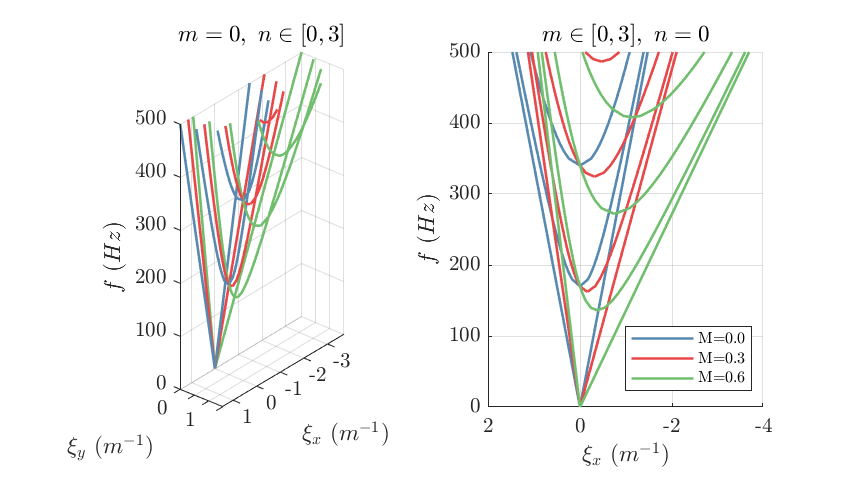
\includegraphics{../matlab/04_dispersion_analysis/dispersion_sound.eps}
  \caption{Acoustic duct mode lines showing the spatial frequency location as a function of temporal frequency, Mach number, and mode number.}
  \label{fig:04_dispersion_sound}
\end{figure}
The lines here represent the solutions to Equation \ref{eqn:02_kzm} for a series of cross-sectional acoustic modes; essentially, these are $f-\xi_x$ planar ``slices'' of the cone-shaped acoustic part of the spectrum, at various discrete values of $xi_y$.
The cross-sectional wavenumbers are $k_x = m\pi/l_x$ and $k_y = n\pi/l_y$ with the vertical spatial frequency, $\xi_y=\pm k_y/2\pi$.
The horizontal spatial frequency is related to the axial wavenumbers, Equation \ref{eqn:02_kzm}, for sound traveling upstream or downstream.
Note that there is a 90$^\circ$ rotation between the duct and beam coordinate systems (Equation \ref{eqn:03_coord_transform}).

The plot on the left of Figure \ref{fig:04_dispersion_sound} shows the acoustic cone when $m=0$ and $n\in [0,3]$ at Mach numbers of 0, 0.3, and 0.6.
Only shown is the positive vertical spatial frequency.
As the vertical spatial frequency of a duct-mode varies only with the mode number $n$ each set occupies a distinct plane, $\xi_y=\pm n/2l_y$.
Only acoustic cone modal lines representing the cut-on duct modes are shown.

The plot on the right of Figure \ref{fig:04_dispersion_sound} shows the acoustic modal lines at $\xi_y=0$ for $n=0$ which fill the inside of the acoustic cone.
The Mach number has a far greater impact on the acoustic cone for the waves traveling upstream.
As the Mach number increases, the cut-on frequency (minimum value in $f$) decreases and the horizontal spatial frequency at the cut-on frequency also decreases.
This effect is more pronounced at higher mode numbers.
The phase velocity of a downstream-traveling acoustic wave can travel upstream.

It may be possible to individually resolve the separate acoustic duct modes using optical wavefronts if the spatial frequency resolution were high enough.
To measure of the vertical mode number, $n$, the spatial frequency resolution would need to be $\Delta\xi_y\ge 1/2l_y$ for a square duct.
With a single beam going through the duct perpendicularly, the axial wave number is directly measurable but its sensitivity is diminished as the temporal frequency is increased.
It would be most sensitive to measuring modes that have just been cut-on.

When the optical beam is passing through a duct at an angle other than $\gamma=90^\circ$ (parallel to the x-axis of the duct), it will measure a combination of the axial wavenumber and the wavenumber along the x-axis (assuming beam is rotating in the $x-z$ plane of the duct),
\begin{equation}
  k^+_{hm} = k^+_{zm}\sin(\gamma)-k_x\cos(\gamma)
\end{equation}
and
\begin{equation}
  k^-_{hm} = -k^-_{zm}\sin(\gamma)+k_x\cos(\gamma) \textrm{.}
\end{equation}
The effective horizontal wavenumber, is related to the spatial frequency via $\xi_x = k^\pm_{hm}/2\pi$.
Figure \ref{fig:04_dispersion_sound_angle} shows the acoustic duct mode lines at Mach number of 0.6 over a range of beam angles.
\begin{figure}
  \centering
  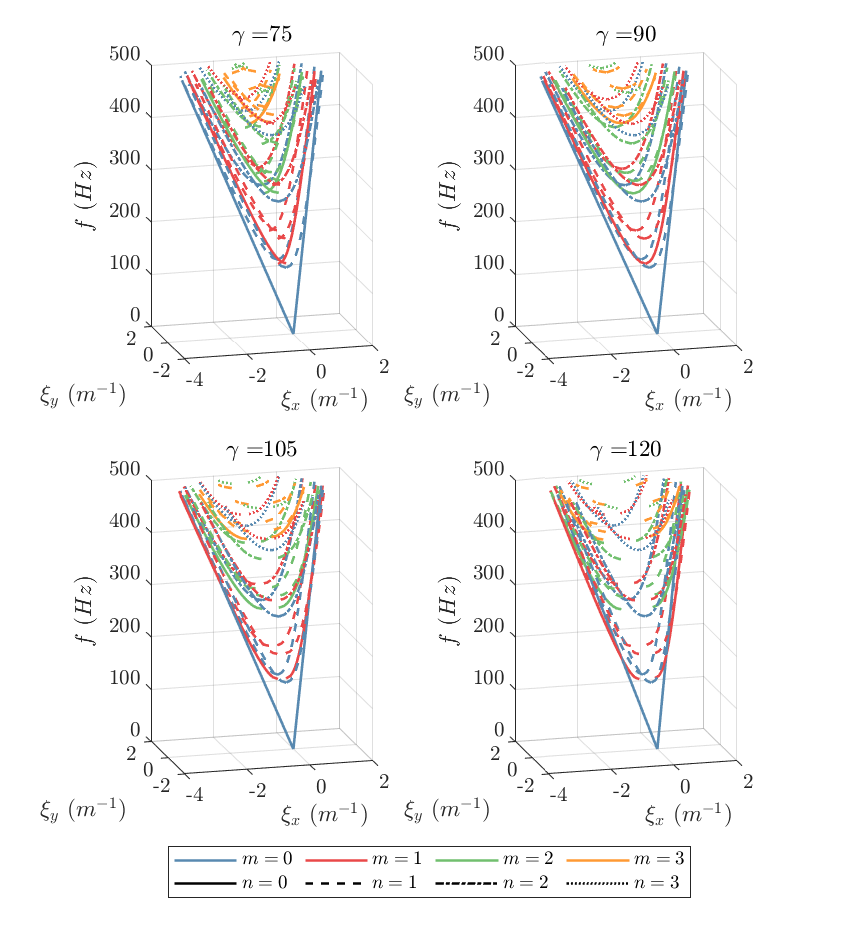
\includegraphics{../matlab/04_dispersion_analysis/dispersion_sound_angle.eps}
  \caption{Acoustic duct mode lines as a function of viewing angle, $\gamma$, at a Mach number of 0.6.}
  \label{fig:04_dispersion_sound_angle}
\end{figure}
As the beam angle is changed from $90^\circ$ the node lines for $m\neq0$ begin to be split at the cut-on frequency with the lines moving outward along $\xi_x$ for angles greater than 90$^\circ$, while for angles less than 90$^\circ$, the node lines cross and travel in the opposite direction.
This causes some of the node lines to begin to overlap near the sonic lines causing constructive interference among the signals which explains the increase in signal observed on the downstream-traveling acoustic waves as the angle increased in Figure \ref{fig:04_dispersion_angle}.
As the angle continues to either 0 or $180^\circ$ the beam is only capable of measuring $k_x$ and $k_y$ with the node lines being parallel to the temporal frequency axis and starting at the cut-on frequency.

\subsection{Signal Aliasing}
In the spectral slices shown in Figure \ref{fig:04_dispersion_xy}, when a signal crosses a plane represented by one of the temporal or spatial Nyquist frequencies (positive or negative) it is transposed to the conjugate Nyquist frequency plane and continues on with the same gradient as before.
This behavior is illustrated in Figure \ref{fig:04_dispersion_tiling} by tiling the base (measured) spectrum, which is shown as the slices of the horizontal moving (stream-wise) disturbances.
\begin{figure}
  \centering
  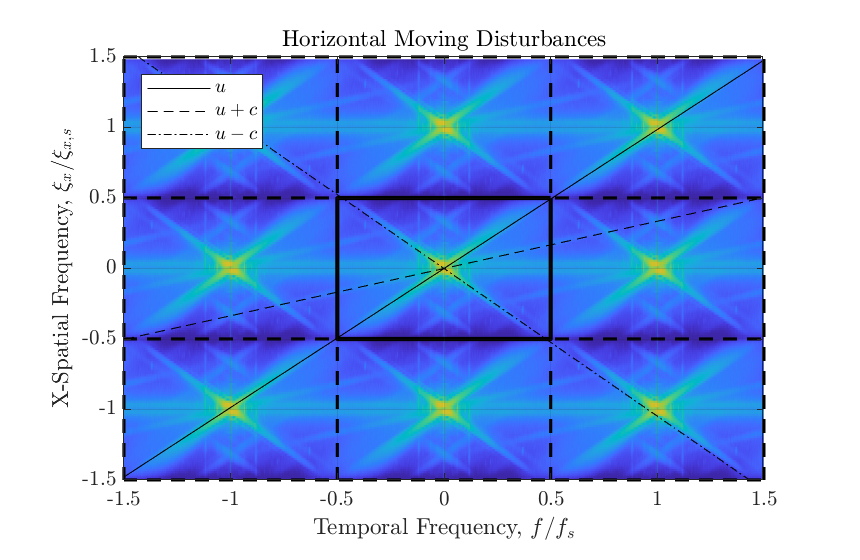
\includegraphics{../matlab/04_dispersion_analysis/dispersion_tiling.eps}
  \caption{Spectrum tiling method to identify aliased data. Shown here as the horizontal moving (stream-wise) disturbance slices, along with lines representing the various characteristic velocities. The thick outline shows the extent of the base spectrum with the thick dashed outlines representing the various tiles of that base spectrum.}
  \label{fig:04_dispersion_tiling}
\end{figure}
The thick outline represents the base spectrum, while the thick dashed outline represent the base spectrum in the tiled positions.
The tiling process for the spectral slices,
\begin{equation}
  S_{xx,T}^{\xi_y=0} = \left[
    \begin{array}{c c c}
      S_{xx}^{\xi_y=0} & S_{xx}^{\xi_y=0} & S_{xx}^{\xi_y=0} \\
      S_{xx}^{\xi_y=0} & S_{xx}^{\xi_y=0} & S_{xx}^{\xi_y=0} \\
      S_{xx}^{\xi_y=0} & S_{xx}^{\xi_y=0} & S_{xx}^{\xi_y=0}
    \end{array}
  \right] \textrm{,}
\end{equation}
where $S_{xx}^{\xi_y=0}$ is the base spectral slice showing the horizontal moving disturbances at $\xi_y=0$ and $S_{xx,T}^{\xi_y=0}$ is the tiled variant.
The temporal frequency is tiled,
\begin{equation}
  \left. f\right|_{tiled} = \left[
    \begin{array}{c c c}
      f-f_s & f & f+f_s
    \end{array}
  \right] \textrm{,}
\end{equation}
where the other frequencies are similarly tiled.
This tiling process works because the negative half ($f<0$) of the spectrum is a duplication of the positive half ($f\ge0$) of the spectrum.
In this research, the spectrum is typically only shown for positive temporal frequencies.
The spectral power at any point in frequency space ($\pm f,\pm\xi_x,\pm\xi_y$) will be equal to the conjugate of that point ($\mp f,\mp\xi_x,\mp\xi_y$).
This tiling process could be used on the full multidimensional spectrum with the tiling occurring on each axis.
While only a three-by-three tiling process was shown, the tiling process in theory needs to be extended to infinity but in practice, with real signals being bandwidth limited, only a finite number of tiles are required.
This process has the effect of artificially increasing the sampling rate \cite{Lynch-2021-DygYkEGU}, especially for spectra that are primarily two-dimensional with structures traveling in only one direction (i.e. supersonic boundary-layers).

Figure \ref{fig:04_dispersion_supersample} shows a zoomed in portion of the Figure \ref{fig:04_dispersion_tiling}.
\begin{figure}
  \centering
  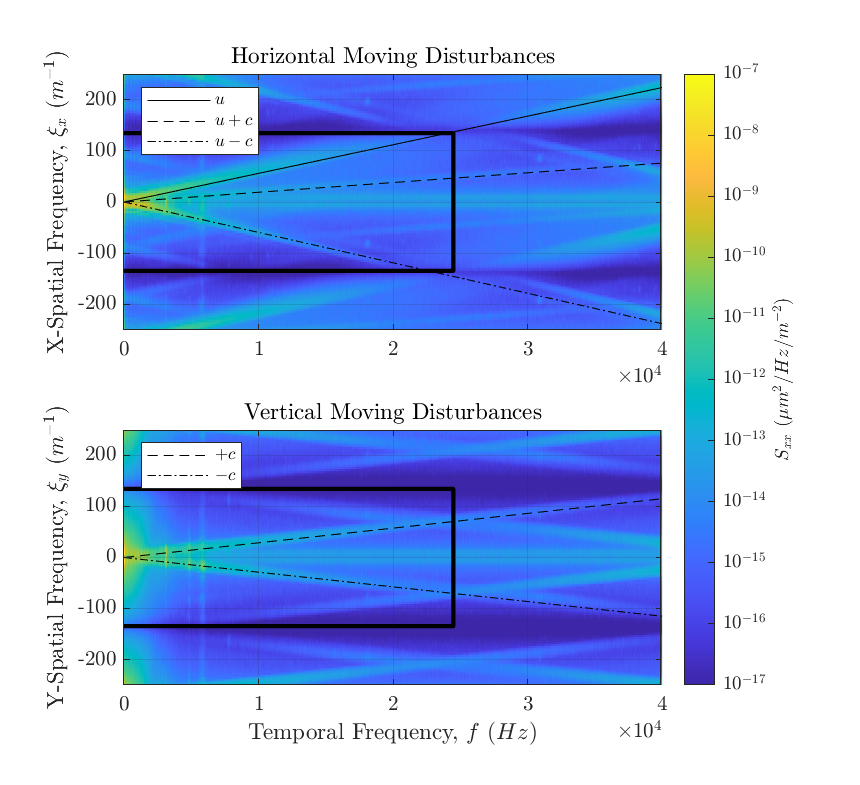
\includegraphics{../matlab/04_dispersion_analysis/dispersion_supersample.eps}
  \caption{Artificially increased temporal sample rate using a dispersion analysis. The black box represents original dispersion plot.}
  \label{fig:04_dispersion_supersample}
\end{figure}
The black box again represents the base spectrum along with lines representing the free-stream velocity and the sonic lines.
When these characteristic lines are extended past the original sample rate, aliased information becomes more apparent.
On the upstream moving disturbance side there is some noticeable aliasing that is present including a significant spike at 18 kHz (-80 $m^{-1}$) while aliased and about 31 kHz (-200 $m^{-1}$) when it has been unaliased.
As that upstream moving acoustic disturbance crosses the spatial Nyquist frequency, the signal strength drops significantly to local background levels.
The boundary layer signal is unfortunately to well aligned with its tiled self for any aliased data to be noticeable.
The vertically moving disturbances have some significant temporal aliasing but little to no spatial aliasing.

There maybe some circumstances when aliased data cannot even be identified, such is likely the case for the boundary layer signal shown in the horizontal moving disturbances plot because the signal is directly inline with its aliased self.
This may also cause an issue when trying to analyze the original spectrum, particularly at the higher frequencies where the aliased data is sufficiently strong and overlapping the true signal.
To avoid this the sample rate velocity,
\begin{equation}
  V_s=f/\xi \textrm{,}
\end{equation}
should sufficiently different enough from the disturbance's characteristic velocity.
This difference will vary for the depending on the spectral width of the signal.
The sample rate velocity of the spectrum in Figure \ref{fig:04_dispersion_supersample} is 176.4 m/s, the free-stream velocity is 174.3 m/s and the boundary layer has a significant spectral with to the signal such that it would be difficult to separate the real and aliased signals.
The upstream-traveling acoustic wave however is a fairly thin signal that is distinguishable from the aliased signal and it has a characteristic velocity of -173.0 m/s.

Figure \ref{fig:04_dispersion_3d_tile} shows a portion of the spectrum that has been tiled three-dimensionally.
\begin{figure}
  \centering
  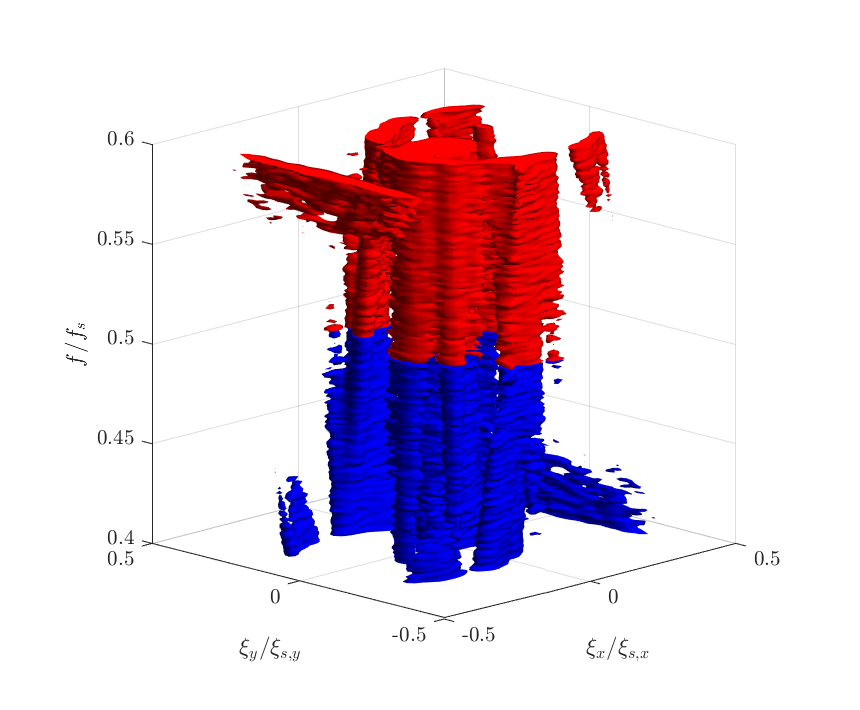
\includegraphics{../matlab/04_dispersion_analysis/dispersion_3d_tile.eps}
  \caption{Three-dimensional tiling of an isosurface of the spectrum at a power of $10^{-14.5}$ $\mu m^2/Hz/m^{-2}$.}
  \label{fig:04_dispersion_3d_tile}
\end{figure}
The power level of the isosurface in this plot is different from those previously shown ($10^{-14.5}$ $\mu m^2/Hz/m^{-2}$).
The level for the previous isosurface plots was chosen because it showed minimal signal aliasing.
In Figure \ref{fig:04_dispersion_3d_tile} the base spectrum is colored in blue and the tiled portion is shown in red.
This plot shows only the portion of the spectrum between 40 and 60\% of the temporal sample rate.
The acoustic cone is the primary structure in this plot that can be seen to having aliasing present.
The `stalactites' that became apparent at higher beam angles are also apparent at this power level and are a continuation from the tiled spectrum above.
With spectra that have significant three-dimensional content, this process is most useful for identifying portions of the signal that are aliased.
There is future work that can be done in both filtering the aliased data and artificially increasing the sample rate of the wavefront measurement.

\section{Summary}
The use of multidimensional spectral estimation on optical wavefronts can provide significant additional insight to the various components that are being measured, including the desired aero-optical signal but also various forms of noise including sound and vibration.
The process of filtering these multidimensional spectra will be discussed in Chapters \ref{chap:06_single_filter} and \ref{chap:07_multiple_filter}.

    % !TEX root = catron-dissertation.tex
\epstopdfsetup{outdir=./images/05_synthetic_wavefront/}

\chapter{Synthetic Wavefront}
\label{chap:05_synthetic}

In the preceding chapter, the way that wavefront data appears in multidimensional spectra was shown using data acquired in Notre Dame’s White Field wind tunnel, for a representative wind-tunnel aero-optical test setup shown in Figure \ref{fig:02_typical_wavefront_system}.
The spectra and accompanying discussion showed how individual sources of optical aberration can be identified in the spectra, such as boundary-layer aero-optical signals, acoustic noise sources, mechanical vibration, etc.
In following chapters of this dissertation, filtering techniques will be presented for extracting or removing signals or noise sources from wavefront data such as shown in Chapter \ref{chap:03_optical_acoustics}.
As a first step towards this objective of developing and examining filtering approaches, this chapter presents methods used to construct a ``synthetic'' wavefront that contains typical optical and aero-optical signals, which will be used to test and examine different filtering techniques described in Chapter \ref{chap:06_single_filter}.

In order to best understand how some basic filters perform on a set of data, a fully known synthetic wavefront was generated such that all of the various components could be generated separately with the combined product filtered and compared to the synthetic wavefront containing only relevant aero-optical data.
This was done by constructing a multidimensional spectrum where each source component was separately generated with parameters that can be modified to alter the output signal as necessary.
The resulting multidimensional spectrum could then be used to create the equivalent spatial- and temporally-resolved wavefront signal in the physical domain by inverse Fourier transforming the spectrum.

This synthetic wavefront generation technique produces a qualitative representation that closely matches the measured wavefront but leaves room for improvement in producing a more physically accurate synthetic wavefront.
It should be stressed that, although physical models for the spectral behavior are presented for some of the signal components, the shape of the spectrum for each signal component was largely constructed to qualitatively match details observed in the spectra for experimental data such as shown in Chapter \ref{chap:03_optical_acoustics}.
This qualitative character to the constructed spectrum for some components should not influence the ability to use the synthesized spectral and wavefront data for examination of filtering approaches, since the constructed data still have the important behaviors exhibited by measured data.

The synthetic wavefront was generated to approximate the same sampling conditions used to acquire the data first presented in Section \ref{sect:03_summary}; these sampling conditions are reasonably typical for Shack-Hartmann wavefront measurements at the time of writing.
The sample rate was 200 m$^{-1}$ (i.e. 200 lenslets/m equivalent in the measurement beam) with 64 ($2^6$) samples in the spatial dimensions and 30,000 Hz with 8192 ($2^{13}$) samples in the temporal dimension.
% The speed of sound was chosen to be 340 m/s, with a Mach number of 0.6, and a boundary layer velocity of 163.2 m/s ($0.8U_\infty$).
Figure \ref{fig:05_dispersion_comp_real} shows the multidimensional spectra estimation of the measured wavefront that was used for the model.
\begin{figure}
  \centering
  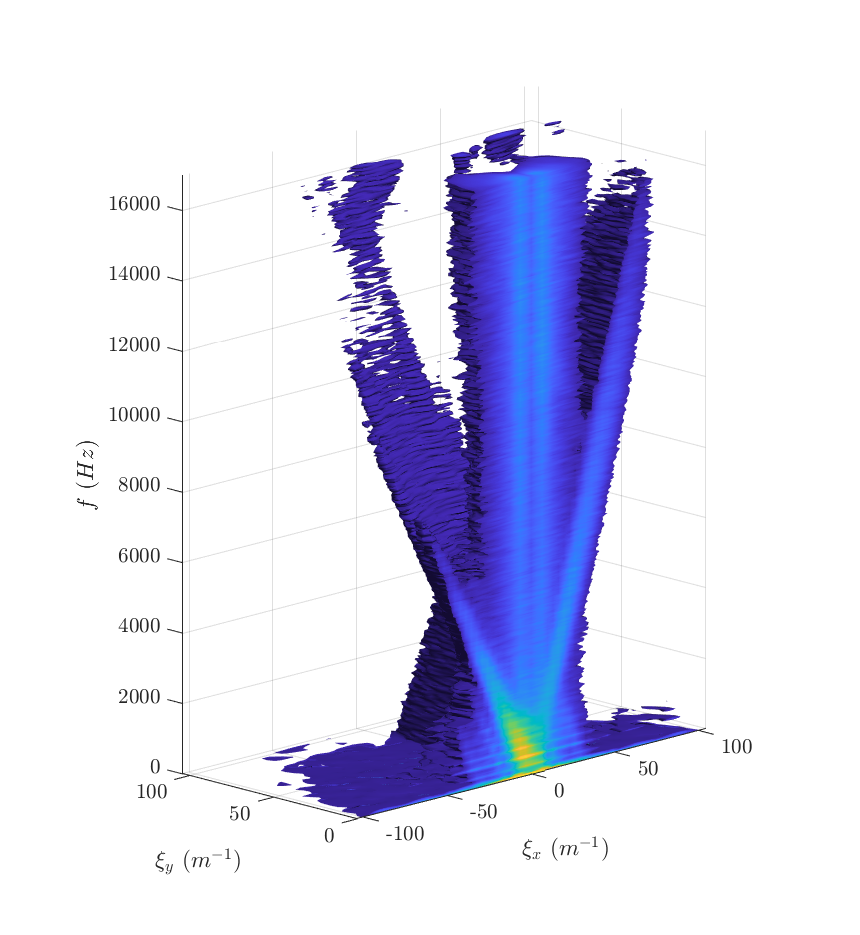
\includegraphics{../matlab/05_synthetic_wavefront/dispersion_comp_real.eps}
  \caption{Multidimensional spectral estimation that the synthetic wavefront is based on.}
  \label{fig:05_dispersion_comp_real}
\end{figure}
The optical wavefront was measured in the University of Notre Dame Whitefield wind tunnel at a Mach number of 0.6 with a 10-inch diameter beam.
The beam angle through the test section was $90^\circ$.

The signals that were assumed to be statistically independent from one another, such as the boundary layer signal, were converted into dimensional space separately and then summed together, while signals that were assumed to be related to one another, such as the sound and vibration components, were first summed together in frequency space.
Figure \ref{fig:05_synthetic_dispersion_input} shows the input dispersion plot with each signal component separately colored.
\begin{figure}
 \centering
 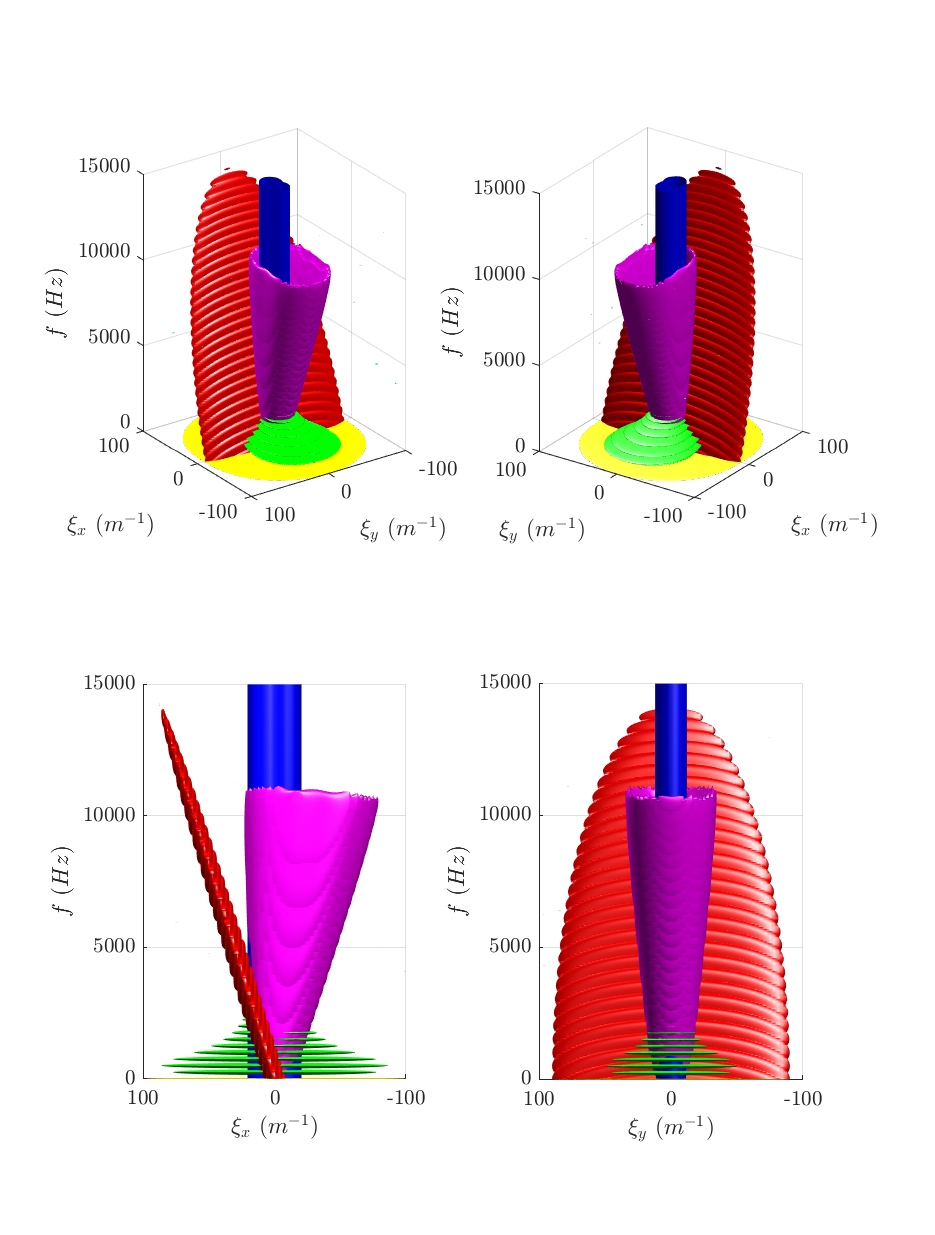
\includegraphics{../matlab/05_synthetic_wavefront/synthetic_wavefront.eps}
 \caption{Synthetic wavefront input dispersion plot of an aero-optical signal and various signal corruption components.  The aero-optical signal is shown in red, the stationary modes in blue, duct acoustics in magenta, blade-passing frequency related corruption in green, slowly varying mean-lensing in yellow, and background in cyan.}
 \label{fig:05_synthetic_dispersion_input}
\end{figure}
The aero-optical signal is shown in red, the stationary modes in blue, duct acoustics in magenta, blade-passing frequency related noise in green, slowly varying mean-lensing in yellow, and background noise in cyan.

\section{General Spectrum Construction}
The general process of developing most of the component signals was to determine an approximate shape, normalize it in the appropriate dimensions, and scale the result by using a function derived from a hyperbola,
\begin{equation}
 \frac{\log_{10}(WF)-b}{b^2}-\frac{\xi_{\rho_N}^2}{a^2} = 1 \textrm{,}
 \label{eqn:05_scaling_hyperbola}
\end{equation}
such that the signal strength at unity of the normalized radial frequency, $\log_{10}(WF(\xi_{\rho_N}=1))$, and the limiting slope, $a/b$, are inputs.
This results in the signal strength of the wavefront being
\begin{equation}
 \log_{10}(WF) = b-\sqrt{\frac{\xi_{\rho_N}^2}{m^2}+b^2} \textrm{,}
 \label{eqn:05_wavefront_strength}
\end{equation}
where
\begin{equation}
 b = \frac{1}{2\log_{10}(WF(\xi_{\rho_N}=1))}\cdot\left(\log_{10}(WF(\xi_{\rho_N}=1))^2-\frac{1}{m^2}\right) \textrm{.}
 \label{eqn:05_wavefront_strength_b}
\end{equation}
% The code used to generate the synthetic wavefront used in this section is shown in Appendix \ref{code:sc_synthetic_wavefront}.

\section{Aero-Optical Signal}
The aero-optical signal was generated to approximate an optical beam passing perpendicularly through a test section with boundary layers on each of the test section walls.
An ellipsoid was chosen to approximate the boundary-layer signal because it is the simplest shape that best resembles the aero-optical signal in Figure \ref{fig:05_dispersion_comp_real}.
This signal was approximated by creating an ellipsoid,
\begin{equation}
  \xi_{\rho_N}^2 = (\xi_{x,R}/a_x)^2+(\xi_{y,R}/a_y)^2+(f_R/a_t)^2
\end{equation}
which had been rotated into the plane representing the boundary-layer's dispersion velocity,
\begin{equation}
  \left[\begin{array}{c} \xi_{x,R} \\ \xi_{y,R} \\ f_R \end{array}\right] = \left[\begin{array}{c c c} \cos\theta_u & 0 & \sin\theta_u \\ 0 & 1 & 0 \\ -\sin\theta_u & 0 & \cos\theta_u \end{array}\right]\left[\begin{array}{c} \xi_{x} \\ \xi_{y} \\ f \end{array}\right]
\end{equation}
where $\theta_u=\tan^{-1}(-1/u_{BL})$.
Equations \ref{eqn:05_wavefront_strength} and \ref{eqn:05_wavefront_strength_b} were then used to calculate the multidimensional spectrum of the boundary layer signal.
% The code used to generate the multidimensional spectrum of the boundary layer signal are shown in lines 18-31 of Appendix \ref{code:sc_synthetic_wavefront} and
The values used are shown in Table \ref{tab:05_boundary_layer}.
In Figure \ref{fig:05_synthetic_dispersion_input} the aero-optical signal is shown in red.
\begin{table}
  \centering
  \caption{Values used in the construction of the multidimensional spectrum for the boundary layer signal}
  \begin{tabular}{c c}
    Variable & Value \\
    \hline \hline
    $a_x$ & 8 \\
    $a_y$ & 90 \\
    $a_t$ & 175 \\
    $m$ & -0.13 \\
    $u_{BL}$ & 163.2 m/s \\
    $\log_{10}(WF(\xi_{\rho_N}=1))$ & -14.5
  \end{tabular}
  \label{tab:05_boundary_layer}
\end{table}

\section{Stationary Mode Signals}
The collection of stationary modes is a temporally constant signal at low spatial frequencies that is often has a cross-section in the plane of spatial-frequencies that is circular.
In the particular case that is being modeled, the stationary modes have a cross-section of two circular regions offset along the $\xi_x$-axis that just overlap one another.
A smooth function was chosen to approximate this overlapping circle type stationary mode,
\begin{equation}
 \xi_{\rho_N} = \frac{\xi_\rho}{\xi_{\rho_0}\sqrt{10-6\cos{(2\xi_\theta+\pi)}}} \textrm{.}
 \label{eqn:05_epicycloid_simple}
\end{equation}
This spectrum for the stationary modes component is shown in blue in Figure \ref{fig:05_synthetic_dispersion_input}.
 % and the relevant code shown in Lines 33-40 of Appendix \ref{code:sc_synthetic_wavefront}.
Table \ref{tab:05_stationary_modes} shows the values used in generating the spectrum.
\begin{table}
  \centering
  \caption{Values used in the construction of the multidimensional spectrum for the signal of the stationary modes}
  \begin{tabular}{c c}
    Variable & Value \\
    \hline \hline
    $m$ & -0.175 \\
    $\xi_{\rho_0}$ & 5 \\
    $\log_{10}(WF(\xi_{\rho_N}=1))$ & -14.5
  \end{tabular}
  \label{tab:05_stationary_modes}
\end{table}

\section{Sound and Vibration Signals}
The sound and vibrating component signals are comprised of two parts.
The first of these is the blade-passing frequency and its harmonic disturbances (shown in green in Figure \ref{fig:05_synthetic_dispersion_input}) and the second is the acoustic duct modes (shown in magenta).

\subsection{Blade-Passing Frequency Disturbance}
Like the stationary modes, the blade-passing frequency disturbances were modeled with the same cross-sectional shape as the stationary mode, Equation \ref{eqn:05_epicycloid_simple}, but as narrow-band discs,
\begin{equation}
  \xi_{\rho_N}^2 = \frac{\sqrt{\xi_x^2+(AR\xi_y)^2}}{\xi_{\rho,BPF}\sqrt{10-6\cos(2\xi_\theta+\pi)}}+\left(\frac{f\pm BPF n}{f_T}\right)^2
  \label{eqn:05_blade_passing_frequency}
\end{equation}
where $AR$ is the aspect ratio of the cross-sectional shape, $n$ is the harmonic number, $f_T$ is the disc thickness, and $\xi_{rho,BPF}$ is
\begin{equation}
  \xi_{rho,BPF} = \frac{\xi_{\rho_0}}{\sqrt{1+\frac{BPF n-BPF}{f_c}}}
\end{equation}
where $f_c$ is the effectively cutoff frequency for modulating the strength of each disc as the harmonic number increased from $n=0.5$ to $n=5$ in steps of 0.5.
% The code for the blade-passing frequency disturbances is shown in Lines 42-60 of Appendix \ref{code:sc_synthetic_wavefront} with
A list of values is shown in Table \ref{tab:05_bpf}.
\begin{table}
  \centering
  \caption{Values used in the construction of the multidimensional spectrum for the blade-passing frequency disturbance}
  \begin{tabular}{c c}
    Variable & Value \\
    \hline \hline
    $AR$ & 1 \\
    $BPF$ & 500 Hz \\
    $f_c$ & 500 Hz \\
    $f_T$ & 100 Hz \\
    $m$ & -0.13 \\
    $\xi_{\rho_0}$ & 20 \\
    $\log_{10}(WF(\xi_{\rho_N}=1))$ & -14
  \end{tabular}
  \label{tab:05_bpf}
\end{table}


\subsection{Acoustic Cone}
The acoustic duct mode disturbances form a cone which in the $f-\xi_x$ plane is defined by the lines $u\pm c$, while in the $f-\xi_y$ plane is defined by the speed of sound.
At each temporal frequency step an ellipse was defined based on the constraining lines and the distance to that ellipse used to calculate a normalized radial frequency,
\begin{equation}
  \xi_{\rho_N}^2 = \frac{\sqrt{(\xi_x-\xi_{x_0})^2+(\xi_y-\xi_{y_0})^2}}{\sqrt{\xi^2_{x_a}\cos^2\xi_\theta+\xi^2_{y_a}\sin^2\xi_\theta-1}} \frac{\sqrt{\xi^2_{x_a}\cos^2\xi_\theta+\xi^2_{y_a}\sin^2\xi_\theta}}{\xi_{\rho_T}} \textrm{,}
\end{equation}
where $\xi_{x_0}$ and $\xi_{y_0}$ are the midpoint between the sonic lines in the x and y directions as a function of $f$, $\xi_{x_a}$ and $\xi_{y_a}$ are the distances from the midpoint to the sonic lines as a function of $f$, and $\xi_{\rho_T}$ is the thickness of the ellipse.
The strength of the disturbance was decreased logarithmically as a function of $|f|$ from $f=0$ to $f=f_s/2$ with Equation \ref{eqn:05_wavefront_strength_b} becoming,
\begin{equation}
  b(f) = \frac{1}{2b_0(f)}\left(b_0^2(f)-\frac{1}{m^2}\right) \textrm{,}
\end{equation}
where
\begin{equation}
  \begin{aligned}
    b_0(f) =& \frac{\log_{10}(WF(\xi_{\rho_N}=1,f=f_s/2))-\log_{10}(WF(\xi_{\rho_N}=1,f=0))}{f_s/2}|f| \\ &+\log_{10}(WF(\xi_{\rho_N}=1,f=f_0)) \textrm{.}
  \end{aligned}
\end{equation}

Two low-pass spatial filters (more discussion in Chapter \ref{chap:06_single_filter}) were used to replicate some of the signal attenuation that happens at the low spatial frequencies in the x-direction.
First a low-pass filter in $\rho$ was used,
\begin{equation}
  WF = WF\sqrt{\frac{1}{1+\left(\frac{\xi_\rho}{\xi_{c_\rho}}\right)^2}} \textrm{,}
\end{equation}
followed by a low-pass filter in the x-direction,
\begin{equation}
  WF = WF\sqrt{\frac{1}{1+\left(\frac{\xi_x}{\xi_{c_x}}\right)^2}} \textrm{.}
\end{equation}
The values used in creating the spectrum are shown in Table \ref{tab:05_cone}.
 % and the code is shown in lines 74-93 of Appendix \ref{code:sc_synthetic_wavefront}.
\begin{table}
  \centering
  \caption{Values used in the construction of the multidimensional spectrum for the acoustic cone disturbance}
  \begin{tabular}{c c}
    Variable & Value \\
    \hline \hline
    $m$ & -0.3 \\
    $\xi_{c_x}$ & 115 m$^{-1}$ \\
    $\xi_{c_\rho}$ & 200 m$^{-1}$ \\
    $\xi_{\rho_T}$ & 8 m$^{-1}$ \\
    $\log_{10}(WF(\xi_{\rho_N}=1,f=0))$ & -13 \\
    $\log_{10}(WF(\xi_{\rho_N}=1,f=f_s/2))$ & -16
  \end{tabular}
  \label{tab:05_cone}
\end{table}

\section{Mean-Lensing Signal}
The mean lensing part of the optical signal is the integrated effect of steady optical aberrations added by lenses, mirror, windows, etc, in the beam path.
The aberrations are effectively random and a physical model cannot be developed for them.
The mean-lensing signal (shown in yellow in Figure \ref{fig:05_synthetic_dispersion_input}) uses same cross-sectional as the blade-passing frequency disturbances and represents the slowly varying spatial disturbance,
\begin{equation}
  \xi_{\rho_N}^2 = \frac{\sqrt{\xi_x^2+(AR\xi_y)^2}}{\xi_{\rho_0}\sqrt{10-6\cos(2\xi_\theta+\pi)}}+\left(\frac{f}{f_T}\right)^2 \textrm{.}
  \label{eqn:05_mean_lensing}
\end{equation}
% The relevant code is shown on lines 62-72 of Appendix \ref{code:sc_synthetic_wavefront} with values shown in Table \ref{tab:05_mean_lensing}.
Table \ref{tab:05_mean_lensing} shows a list of the values used in creating this component of the wavefront signal.
\begin{table}
  \centering
  \caption{Values used in the construction of the multidimensional spectrum for the mean-lensing disturbance}
  \begin{tabular}{c c}
    Variable & Value \\
    \hline \hline
    $AR$ & 0.55 \\
    $f_T$ & 50 Hz \\
    $m$ & -0.5 \\
    $\xi_{\rho_0}$ & 25 \\
    $\log_{10}(WF(\xi_{\rho_N}=1))$ & -14.5
  \end{tabular}
  \label{tab:05_mean_lensing}
\end{table}

\section{Background Noise Signal}
Background noise in the wavefront data originates from sources which are random in nature.
The background noise disturbance (with a few small spots shown in cyan in Figure \ref{fig:05_synthetic_dispersion_input}) was simulated using normally distributed random noise with a mean noise level, $\mu(\log_{10}(WF))=-18$, and deviation, $\sigma(\log_{10}(WF))=0.75$.
% The relevant code is shown in lines 95-100 of Appendix \ref{code:sc_synthetic_wavefront}.

\section{Synthetic Wavefront Creation}
A synthetic signal can be created from a power spectrum by solving for $x$ in Equation \ref{eqn:04_basic_sxx} and using the Inverse Fast Fourier Transform,
\begin{equation}
 x(t) = \real\left[\ifft\left\{\sqrt{S_{xx}\cdot N\cdot f_{samp}}\cdot\exp{i\phi}\right\}\right] \textrm{,}
 \label{eqn:05_ifft}
\end{equation}
where $\real$ is the real component and $\phi$ is a random set of phases for each point in the measurement space.
As shown previously this relation can be extended into $n$-dimensions,
\begin{equation}
 f(\mathbf{x}) = \real\left[\ifftn\left\{\sqrt{\mathbf{S_{xx}}\cdot\prod{\overrightarrow{N}\cdot \overrightarrow{f}_{samp}}}\cdot\exp{i\mathbf{\phi}}\right\}\right] \textrm{.}
 \label{eqn:05_ifftn}
\end{equation}
Care should be taken when constructing the random set of phases, as the zero-frequency component has zero phase, $\phi(0,0,0) = 0$, and the phases on either side of it are conjugates of one another, $\phi(\pm\xi_x,\pm\xi_y,\pm f)=-\phi(\mp\xi_x,\mp\xi_y,\mp f)$.
% The code for creating a wavefront from a multidimensional spectrum is shown in lines 196-202 of Appendix \ref{code:sc_synthetic_wavefront} and is specifically creating the wavefront for the aero-optical signal but other signals are generated using the same basic code.
% Note that the first three lines are to get the set of phases properly configured that creates conjugate phases rotated about the origin.

It was assumed that the aero-optical signal, the stationary modes, the background noise, and the sound and vibration combination of modes were statistically independent of one another and, as such, could be separately transformed into physical space.
The components of the sound and vibration sources, the blade-passing frequency, the acoustic cone, and the mean-lensing, were assumed to be related to one another and thus were summed together in frequency space prior to being transformed into physical space.
Once the separate components were in physical space the total wavefront was obtained by summing up the separate components with the aero-optical signal saved along side the total wavefront.
Some frames from the synthetic wavefront are shown in Figure \ref{fig:05_synthetic_frames} with the total wavefront shown on top and the aero-optical only signal shown on the bottom.
\begin{figure}
 \centering
 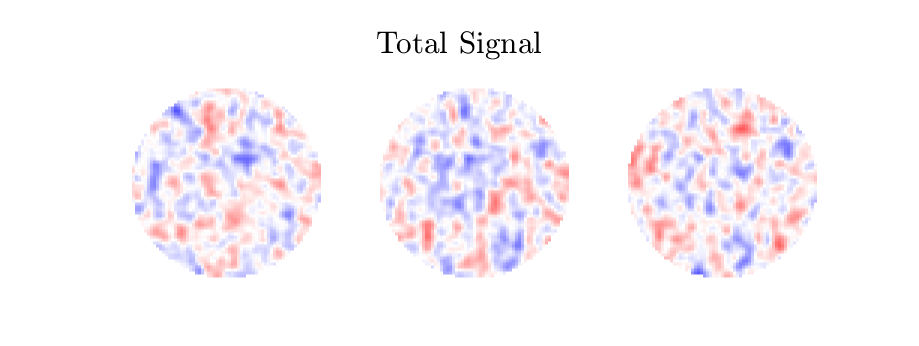
\includegraphics{../matlab/05_synthetic_wavefront/synthetic_frames_total.eps}
 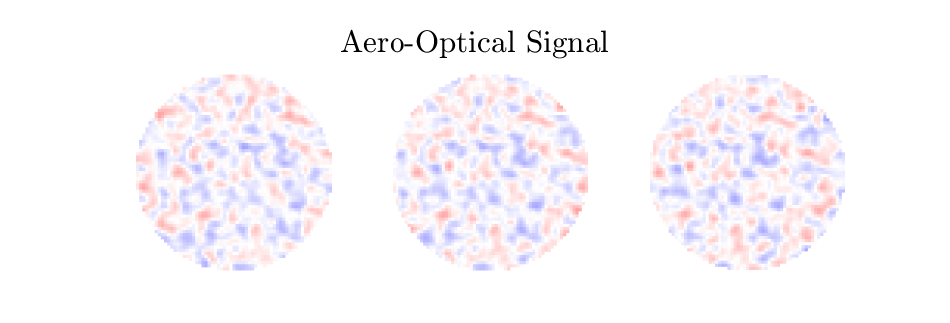
\includegraphics{../matlab/05_synthetic_wavefront/synthetic_frames_ao.eps}
 \caption{Sample frames from the synthetic wavefront with the total wavefront signal on top and the aero-optical only signal bottom.  Flow is from right to left.}
 \label{fig:05_synthetic_frames}
\end{figure}
Flow is from right to left.
The aero-optical signal is noticeable to some degree in the total wavefront signal, but can be overpowered by the various noise sources.

\section{Comparison to Measured Data}
A multidimensional spectral plot of the total synthetic wavefront is shown in Figure \ref{fig:dispersion_comp_synthetic}.
\begin{figure}
 \centering
 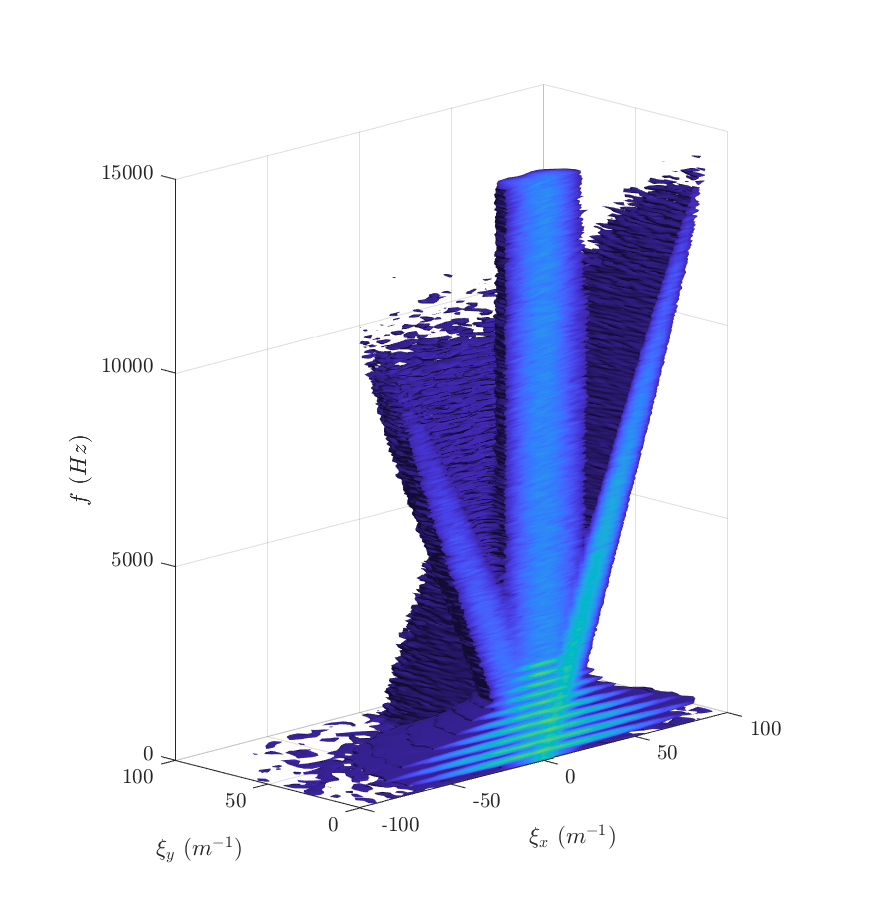
\includegraphics{../matlab/05_synthetic_wavefront/dispersion_comp_synthetic.eps}
 \caption{Synthetic wavefront output dispersion plot of an aero-optical signal and various signal corruption components.}
 \label{fig:dispersion_comp_synthetic}
\end{figure}
In this view the aero-optical signal is more noticeable but there still remains some significant overlap with the various noise sources.
While the mean-lensing component is not as visible in this isosurface, the rest of the dispersion plot in a good representation of the input dispersion plot shown in Figure \ref{fig:05_synthetic_dispersion_input}.
The blade-passing frequency was depicted as symmetric in the synthetic wavefront while measured data (shown in Figure \ref{fig:04_dispersion_3d}) shows more signal on the side traveling in the direction of flow.
The harmonics of the BPF are more on the upstream traveling side of the dispersion and are a little less pronounced in the measured data.
The total synthetic wavefront has a $\opdrms$ of $0.0112\pm0.0006\mu m$ with the aero-optical only signal having a $\opdrms$ of $0.0073\pm0.0003\mu m$.
The measured wavefront presented in Figure \ref{fig:04_dispersion_3d} had a $\opdrms$ of $0.0874\pm0.0263\mu m$.
The overall $\opdrms$ of the synthetic wavefront was $12.8\%$ when compared to the measured wavefront indicating that the algorithms used to generate the wavefront are not representative of reality and can provide a future path of research in order to produce more realistic synthetic wavefronts.

    % !TEX root = catron-dissertation.tex
\epstopdfsetup{outdir=./images/06_single_sensor_filtering/}

\chapter{Single Sensor Filtering Techniques}

\textcolor{red}{Show some dispersions of POD modes and discuss whether or not POD filtering maybe a viable option.}

A filter is a function, $G(\mathbf{\omega})$, that describes the gain a signal will experience in frequency space.
In the simplest case, the filtered signal is the inverse Fourier transform of the gain multiplied by the Fourier transform of the signal.
Additionally, a windowing function, $W(\mathbf{x})$, can be used to help suppress finite sampling effects,
\begin{equation}
 f_F(\mathbf{x}) = \real\left(\frac{\ifftn[G(\mathbf{\omega})\cdot\fftn\{f(\mathbf{x})\cdot W(\mathbf{x})\}]}{W(\mathbf{x})}\right) \textrm{,}
 \label{eqn:06_filter_function}
\end{equation}
where $f$ is the signal function and $f_F$ is the filtered signal.
Depending on the windowing function some data could be destroyed during this process if there is a zero present due to the possibility of dividing by zero.

A basic MATLAB code for applying a filter to a wavefront using a separate function for both generating and applying the gain function which is presented in Listing \ref{code:sc_basic_wavefront_filters}.
This code generates a windowing function as described by Equations \ref{eqn:04_hann_window}, \ref{eqn:04_window_sep}, and \ref{eqn:04_window_space_arb}.
The temporal windowing function was generated with an additional two terms such that the end points which are equal to zero could be removed to prevent the first and last frames from being destroyed.
Likewise, the spatial window used the arbitrary aperture function which ensures that all of the points inside of the aperture are non-zero.
In some cases, a windowing function was not used due to filtered wavefront having a far greater magnitude in some places despite the precautions used.
The filter presented in this code sample is a second order temporal high-pass filter with a cut-off frequency of 2000 Hz.
The function \lstinline{WFfilter} takes input based on a normalized cut-point in reference to the sample rate.

\section{Temporal Filter Methods}
The methods presented in this section are based on Butterworth filters \cite{Butterworth-1930-DvDrjKha} but could easily be extended to other types of filters.
The basic gain function,
\begin{equation}
 G(f) = \frac{1}{\sqrt{1+\left(\frac{f}{f_c}\right)^{\pm2n}}} \textrm{,}
 \label{eqn:06_butterworth}
\end{equation}
where $f_c$ is the cut-off frequency, $n$ is the filter order (number of filters in a series), and $\pm$ represents either a low-pass ($+$) or high-pass ($-$) filter.
In this particular formulation, only the magnitude is attenuated, circuit based Butterworth filters or their digital copies will have some variable phase attenuation as well.
Additionally, a band-pass filter can be constructed by placing a low-pass in series with a high-pass filter and a band-stop by placing the two types in parallel.

As a large portion of the wavefront contamination is at low frequencies, a high-pass filter is the most useful in temporal space for removing unwanted contamination, as shown in Figure \ref{fig:06_filter_temporal}.
\begin{figure}
 \centering
 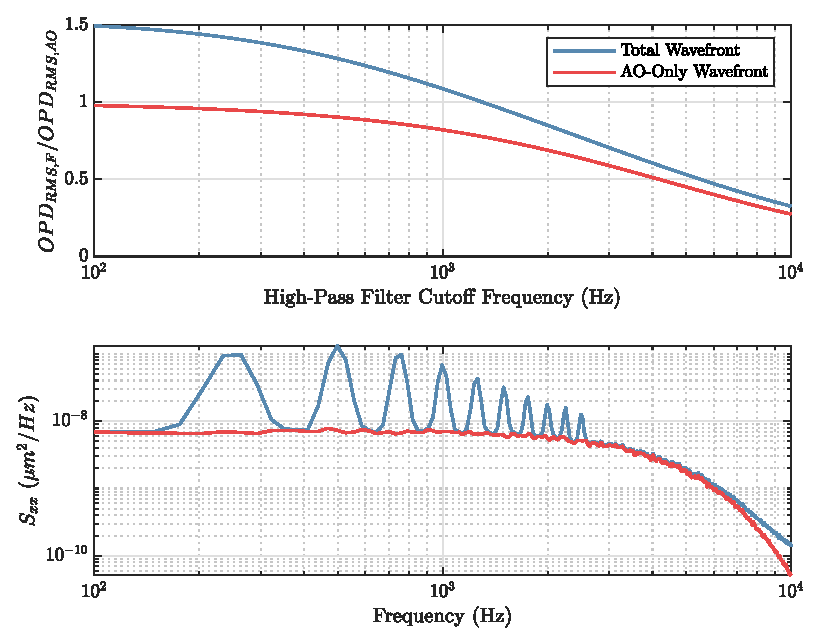
\includegraphics{../matlab/06_single_sensor_filtering/filter_temporal.eps}
 \caption{OPD time-averaged spatial-RMS of high-pass temporal filters relative to the aero-optical only unfiltered wavefront.}
 \label{fig:06_filter_temporal}
\end{figure}
This figure shows the time-averaged spatial-RMS of both the total and aero-optical only wavefronts with various cut-off high-pass filters relative to that of the aero-optical only wavefront unfiltered.
The total wavefront ratio crosses unity around 1200 Hz, which is about halfway between the second and third harmonic of the blade-passing frequency in this simulated wavefront.
While approximately 75\% of the aero-optical signal remains at this cut-off frequency, that difference is made up by the remaining contamination.
This can provide a computationally cheap way estimating the aero-optical portion of the wavefront for calculations that rely on the spatial-RMS of a wavefront.
While it is easy to determine a cut-off frequency for this synthetic wavefront, a measured wavefront will likely take some knowledge or expectation of the contamination that is present in the measurement.

% \ref{tab:test}
% \begin{table}
% \centering
% \caption{Test Table}
% \input{../matlab/04_basic_filtering/filter_temporal.txt}
% \label{tab:test}
% \end{table}

An example of band-pass and band-stop filtering is shown if Figure \ref{fig:06_filter_temporal_bandpass}.
\begin{figure}
 \centering
 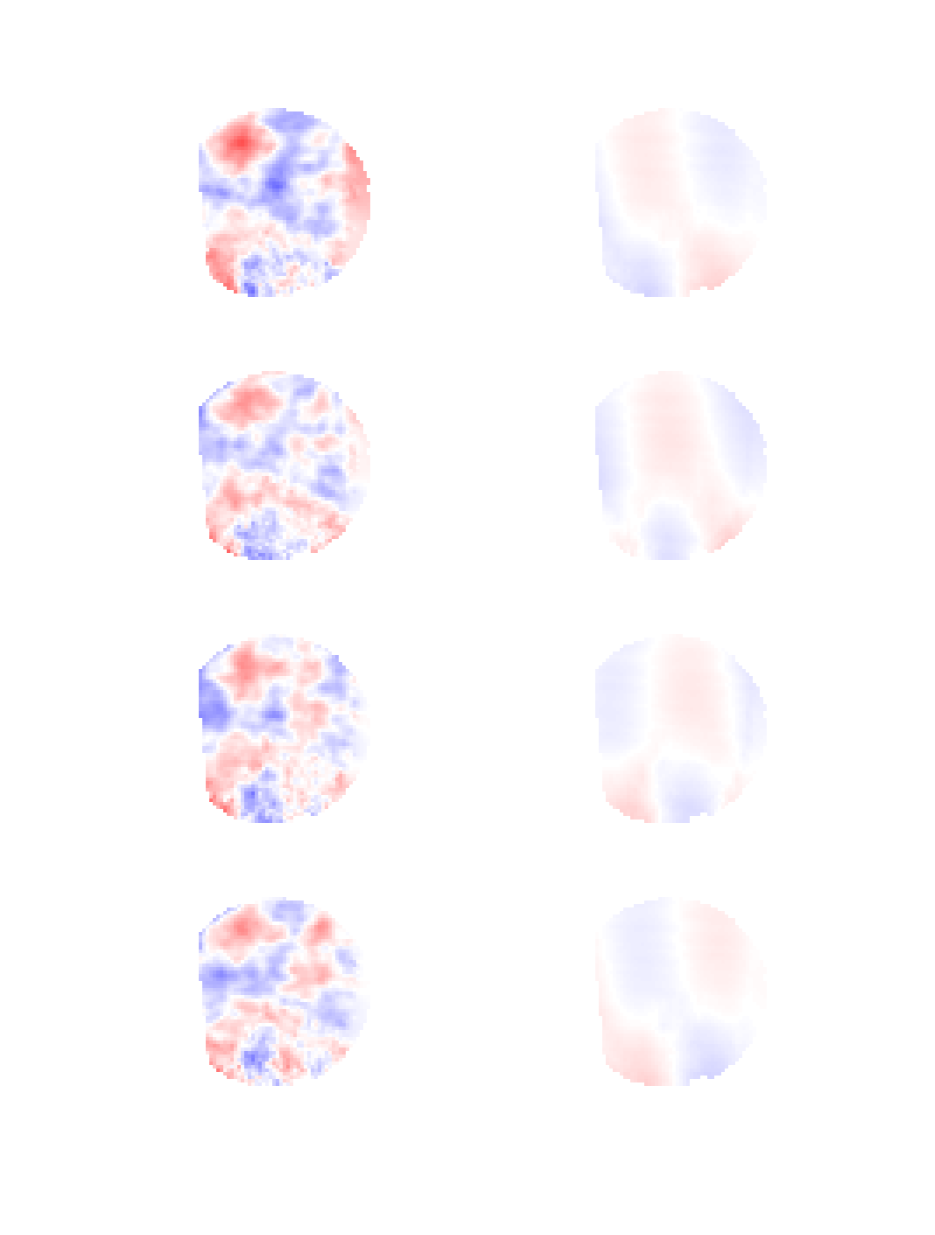
\includegraphics{../matlab/06_single_sensor_filtering/filter_temporal_bandpass.eps}
 \caption{Measured wavefronts filtered at the blade-passing frequency (532$\pm$10 Hz).  The left column is band-stop filtered while the right is band-pass filtered.}
 \label{fig:06_filter_temporal_bandpass}
\end{figure}
The figure shows measured data that is band-stop filtered in the left column and band-pass filtered in the right column in several different frames.
The flow is from right-to-left and the band-pass filtered wavefront clearly shows upstream-moving optical disturbances associated with acoustic duct modes traveling upstream from the fan.
The band-stop shows a much slower moving optical disturbance that is in general moving in the direction of the flow, but it still possess the optical disturbances of the blade-pass frequency harmonics.

One thing of note, MATLAB's builtin filter functions only work in one-dimension of frequency space and are unable to determine the direction that a signal is traveling.
They also only apply the filter to the positive frequencies and zero-out the negative ones which both reduces the signal by two and also switches all disturbances to moving in the same direction.
So even for a filter that operates in one-dimension, it is best to apply the filter over both positive and negative frequencies to the n-dimensional Fourier transform in order to preserve the direction of travel of a signal.
This additionally allows several filters to be applied in series with one another without having to perform a Fourier and inverse Fourier transform for each successive filter.
\textcolor{red}{I should maybe show this matlab filter issue in an appendix.}

Some additional uses of temporal filters would be in sizing and/or designing an adaptive optics system.
A low-pass filter with a cut-off at the bandwidth of either a fast-steering or deformable mirror would help determine the signal that a system would need to reject.
A control system may need to have the bandwidth reduced in order to keep a mirror's travel within limits.
While a high-pass filter would inform designers of the remaining optical aberrations that cannot be corrected.




\section{Upstream/Downstream Moving}
For the filtering of upstream and downstream moving optical disturbances a logistic function was chosen,
\begin{equation}
 f(x) = \frac{1}{1+\exp\{-kx\}} \textrm{.}
 \label{eqn:06_logistic}
\end{equation}
This function needs to be expanded into two-dimensions ($x$ and $t$) with the filter ideally returning a value of one in both the first and third quadrants and zero otherwise for a filter outputs disturbances moving in the direction of flow.
To accomplish this the logistic curve in each dimension is scaled and offset to output values between negative one and positive one,
\begin{equation}
 G_t(f) = \frac{2}{1+\exp\{-k_tf\}}-1
 \label{eqn:06_logistic_time}
\end{equation}
and
\begin{equation}
 G_x(\xi_x) = \frac{2}{1+\exp\{\pm k_x\xi_x\}}-1 \textrm{,}
 \label{eqn:06_logistic_space}
\end{equation}
where $\pm$ determines whether the filter is obtaining upstream traveling disturbances ($+$) or downstream traveling ($-$).
These two gain functions are then multiplied together and scaled to output values between zero and one,
\begin{equation}
 G(\xi_x,f) = \frac{(G_t\cdot G_x)+1}{2} \textrm{.}
 \label{eqn:06_up_down_filter}
\end{equation}
As the values of $k_x$ and $k_t$ go to infinity an ideal case is obtained.
Downstream traveling disturbances have a gain of one in the first and third quadrants, zero in the second and forth quadrants, and a value of $1/2$ when either frequency is zero.

The dispersion analysis using an ideal downstream moving filter on the synthetic wavefront is shown in Figure \ref{fig:06_filter_downstream} along side the dispersion of the unfiltered wavefront.
\begin{figure}
 \centering
 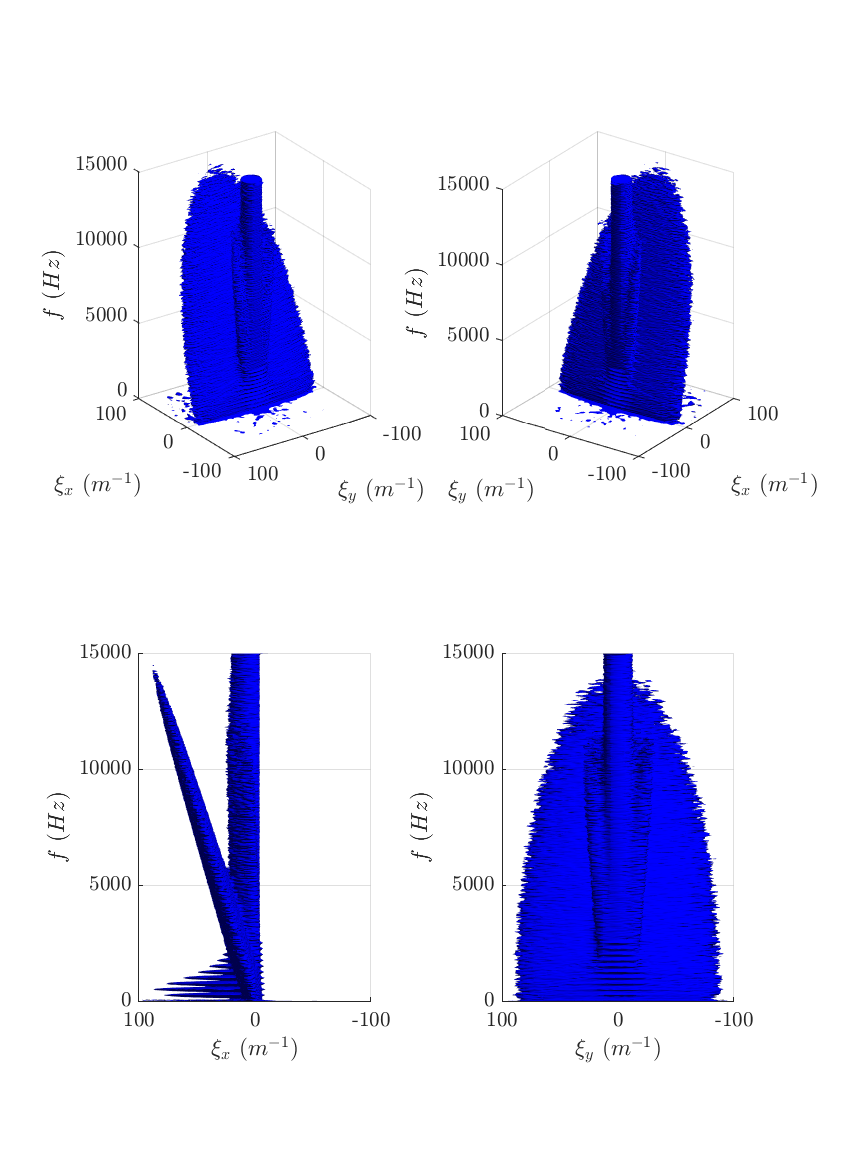
\includegraphics{../matlab/06_single_sensor_filtering/filter_downstream.eps}
 \caption{Dispersion isosurface of the synthetic wavefront with a downstream filter in place.}
 \label{fig:06_filter_downstream}
\end{figure}
All of the upstream traveling disturbances are removed and the disturbances at $\xi_x=0$ m$^{-1}$ are significantly reduced.
Some of the stationary modes remain while only the acoustic and vibration signals that are propagating in the direction of flow remain.
The aero-optical signal is clipped slightly at $\xi_x=0$ due to the spatial width of the signal.
The ratio of the time-averaged spatial-RMS of the filtered signal when compared to the aero-optic only signal was 1.24 while the unfiltered ratio was 1.53.
When the filter was applied to only the aero-optic signal the ratio was 0.96.
This filter method will retain any disturbance that is traveling in the direction of flow.
Even with an ideal filter there is some slight attenuation of the aero-optical signal due to signal having some spectral width that crosses into upstream-moving portion of the dispersion plot.


\section{Velocity Filtering}
The dispersion plot shows flow structures that are traveling at a given speed as having a constant slope.
A plane in the dispersion plot can be used to measure a flow structure's velocity in both $x$ and $y$-directions.
The distance from any given point in the dispersion plot to a plane described by the velocities $v_x$ and $v_y$ can be computed by
\begin{equation}
 d = \frac{|v_x\xi_x+v_y\xi_y-f|}{\sqrt{v_x^2+v_y^2+1}} \textrm{.}
 \label{eqn:06_dist_point_2_plane}
\end{equation}
A low-pass or high-pass filter can then be used to retain only disturbances that are traveling at that velocity, or to exclude those disturbances respectively.

A low-pass velocity-filter of the synthetic wavefront is shown in Figure \ref{fig:06_filter_velocity}.
\begin{figure}
 \centering
 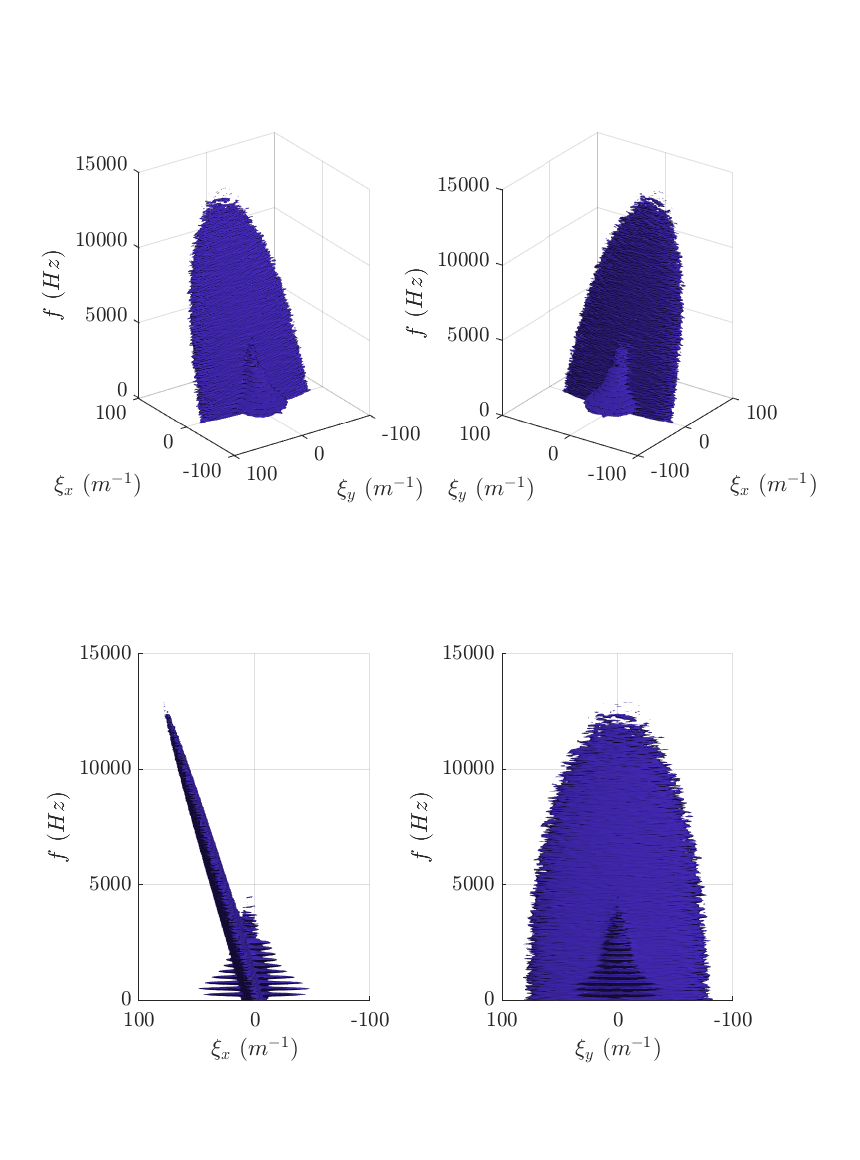
\includegraphics{../matlab/06_single_sensor_filtering/filter_velocity.eps}
 \caption{Dispersion isosurface of the synthetic wavefront with a low-pass velocity-filter in place.}
 \label{fig:06_filter_velocity}
\end{figure}
The filtered dispersion plot shows primarily only the aero-optic signal remains with some additional low-frequency content from the blade-passing frequency and harmonic disturbances as well as some stationary and acoustic disturbances.
The ratio of the time-averaged spatial-RMS relative to that of the aero-optical only signal went from 1.53 in the unfiltered case to 1.01 in the filtered case.
This method can provide a very effective way in quickly estimating the clean spatial-RMS of a contaminated wavefront.

Another use of the synthetic wavefront is measuring the speed of a broadband disturbance such as the aero-optical signal of a boundary layer.
This is done by finding the velocity that maximizes the output spatial-RMS of the velocity filter, see Figure \ref{fig:06_filter_velocity_measure}.
\begin{figure}
 \centering
 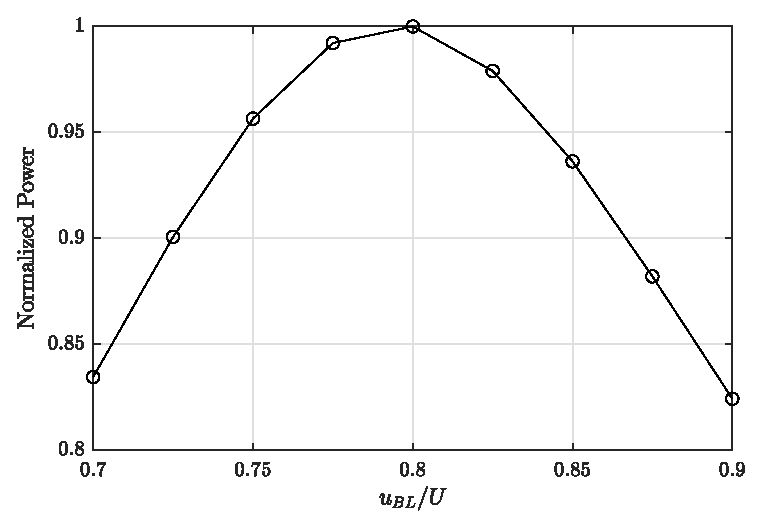
\includegraphics{../matlab/06_single_sensor_filtering/filter_velocity_measure.eps}
 \caption{Velocity low-pass filter used to determine the mean disturbance velocity.  The maximum value corresponds with the actual value used in the creation of the synthetic wavefront.}
 \label{fig:06_filter_velocity_measure}
\end{figure}
In this case boundary layer speed was determined to be 163 m/s which corresponds to the design velocity of the synthetic signal of $0.8U$.
If the velocity range used is to large, a false result can be obtained due to the inclusion of disturbance structures not related to the aero-optical signal.
For signals that have a mean-velocity component that is not aligned with an axis both velocity components can be varied as shown in Figure \ref{fig:06_filter_velocity_real}.
\begin{figure}
 \centering
 \includegraphics{../matlab/06_single_sensor_filtering/filter_velocity_real.eps}
 \caption{Velocity low-pass filter used to determine the mean disturbance velocity of measured data presented in Figure \ref{fig:06_dispersion_real}.  The velocity in the x-direction was measured to be 207 m/s and -17 m/s in the y-direction.}
 \label{fig:06_filter_velocity_real}
\end{figure}
In this case a variable low-pass velocity filter was employed with a high-pass spatial filter operating in the radial direction.
This helped eliminate some of the low-frequency stationary disturbances as well as some of the disturbances related to the blade-passing frequency.
The velocity was measured using the optical disturbances in the dispersion plot to be approximately 207 m/s in the x-direction and -17 m/s in the y-direction.

\section{Basic Filter Summary}
Three different basic wavefront filters were shown and discussed in this chapter.
The temporal filter is most useful when separating an optical wavefront into frequency bands.
Adaptive optics system performance can be evaluated by using both high-pass and low-pass temporal filters.
High-pass filters can be used to determine a systems performance that cannot be corrected while low-pass filters can be used to sizing the travel of active optical components.
Band-pass filters are helpful in analyzing a wavefront over a narrow-band to examine the optical aberrations at specific frequencies that significantly contribute to the overall optical disturbance.

Filters that separate upstream and downstream-moving disturbances are useful as most of the optical contamination comes from acoustic signals that are traveling upstream form a wind-tunnel fan.
These filters would also be useful for separating out an aero-optical signal that has a broad range of velocities that can occur in a span wise measurement of a boundary layer.
\textcolor{red}{Use some of sontag's data and site his dissertation.}

The velocity filter is the most useful for isolating the aero-optical portion of a wavefront measurement given the aero-optical signal has a fairly narrow and constant velocity range.
By using this filter to maximize the power over a range of velocities it can be used to measure the speed in both x and y-directions of an optical disturbance.

    % !TEX root = catron-dissertation.tex
\epstopdfsetup{outdir=./images/07_multiple_sensor_filtering/}

\chapter{Combination of Filters}
\label{chap:07_multiple_filter}
% \textcolor{red}{
%   \begin{itemize}
%     \item Figure 7.2 - ylabel OPDRMS(t)
%     \item Figure 7.3,7.4 - Backward Moving Filter
%     \item Add figure showing the combined Velocity_LSE_MSPOD multidimensional spectrum
%   \end{itemize}
% }

The previous chapter investigated a series of filters that were applied in a singular fashion to a set of optical wavefronts.
This chapter will discuss combining several of these filters together in series.


\section{Velocity and LSE-SPOD Filter}
In addition to the LSE-SPOD filter using all 16 additional sensors that was shown in Chapter \ref{chap:06_single_filter}, a velocity filter was applied to the wavefront first.
Table \ref{tab:07_lse_mspod_table_vel} shows the summary of these filters when used separately or together.
The LSE-SPOD was shown previously to remove vibration noise from wavefront measurements with an approximately 85\% reduction in $\opdrms$ at Mach of 0.3 \cite{DeLucca-2014-RAJvGdv7}.
Similar results were observed using the combination of optical tip/tilt removal and LSE-SPOD on both single dimension (temporal) and multidimensional spectra.
Optical tip/tilt removal alone accounted for a 78.6\% reduction in $\opdrms$, with a combination of 16 microphones and accelerometers and the LSE-SPOD bringing the reduction in $\opdrms$ to 83.9\% at Mach of 0.3.
The combination of tip/tilt removal and the velocity filter showed a greater reduction of 82.3\%.
At a Mach number of 0.5, the use of optical tip/tilt removal, the velocity filter, and 16 sensors in LSE-SPOD, the $\opdrms$ was brought down to 0.0181 $\mu m$ and stilled showed a significant amount of narrow-band signals (see Figure \ref{fig:07_lse_spod} and \ref{fig:07_lse_mspod}).
This is about a 30\% reduction when compared with the other filters used in Table \ref{tab:08_filter_summary}, and represents almost entirely an additional reduction in contamination to the aero-optical signal by removing the broadband disturbances.
This was also significantly above the estimated $\opdrms$ of 0.0142 $\mu m$ for the $M=0.6$ case (See Section \ref{sect:02_BL_OPD} and \cite{Gordeyev-2014-jcJndkHM}).
\begin{table}
  \centering
  \caption{$\opdrms$ ($\mu m$) comparison of using LSE-MSPOD filtering process when combined with a velocity filter.}
  \input{../matlab/07_multiple_sensor_filtering/lse_mspod_table_vel.txt}
  \label{tab:07_lse_mspod_table_vel}
\end{table}

With the LSE-SPOD method the more sensors that were used in the filtering process the greater the reduction in the $\opdrms$, as can be seen in Figure \ref{fig:08_lse_summary}.
\begin{figure}
  \centering
  \includegraphics{../matlab/08_conclusion/lse_summary.eps}
  \caption{Percent reduction in $\opdrms$ from the tip/tilt removed case using LSE-SPOD filtering.}
  \label{fig:08_lse_summary}
\end{figure}
The combination of the DAQ and preamplifier used for the duct-mounted microphones had a significantly lower dynamic range when compared to the other sensors, possibly leading to a diminished reduction in the performance of the four-sensor filtering.
The signal reduction using all 16 sensors was fairly uniform with frequency, as shown in Figure \ref{fig:08_lse_mspod_freq}.
\begin{figure}
  \centering
  \includegraphics{../matlab/07_multiple_sensor_filtering/lse_mspod_freq.eps}
  \caption{Reduction in $\opdrms(t)$ as a function of temporal frequency using 16 sensors with LSE-SPOD in the M=0.5 case when compared to tip/tilt removal.}
  \label{fig:08_lse_mspod_freq}
\end{figure}
On average there was a 1.3dB/Hz reduction in the $\opdrms$ with slight peaks at some of the significant narrow-band signals.
At the blade-passing frequency (517 Hz) there was a 2dB/Hz reduction and for the narrow-band signals around 3 and 6 kHz there was a 3dB/Hz reduction.
The first, second, and third harmonics of the blade-passing frequency, at 1034 Hz, 2068 Hz, and 4136 Hz, had a below average reduction in the signal.

While the use of additional sensor measurements to aid in filtering of optical wavefront measurements using LSE-SPOD showed little benefit in this study (at least compared to the single sensor filtering techniques), it could show significant benefit in future measurements.
Specifically, for measurements with models that are likely to create narrow-band signal noise, additional sensor information could be used in conjunction with a baseline filter for determining which narrow-band signals that need to be retained in the spectrum.


\section{Backward, Velocity, and Baseline Filter}
Among the filters discussed, three are useful for isolating aero-optical signals from a wavefront.
The first of these is a filter for separating the portion of the optical disturbances that are moving either upstream or downstream to the flow (Section  \ref{chap:06_up_down_filter}).
An undesirable effect of this filter is that it may remove some of the aero-optical signal, which can happen to the boundary-layer signal\footnote{These low frequency aero-optical disturbances may be a combination of the outer boundary layer and free-stream turbulence.} at low temporal frequencies.
The second useful filter is the low-pass velocity filter which preserves the signal that is moving within a narrow velocity range (Section \ref{chap:06_velocity_filter}).
The third is the baseline estimator (Section \ref{chap:06_baseline}), which removes the narrow-band signals associated with the blade-passing frequency and its harmonics, the mean-lensing component, and other temporally narrow-band signals.
However, some of these removed narrow-band signals could include part of the aero-optical signal of the wind-tunnel model.

Figure \ref{fig:08_dispersion_filters} shows the multidimensional spectra of the output of these three filters individually plus the spectra of these three filters combined.
\begin{figure}
  \centering
  \includegraphics{../matlab/08_conclusion/dispersion_filters.eps}
  \caption{Multidimensional spectra of three single sensor filtering techniques and a combination filter.}
  \label{fig:08_dispersion_filters}
\end{figure}
The backward moving filter, that removes all upstream-moving disturbances (Figure \ref{fig:08_dispersion_filters} top left), does remove some of the boundary-layer signal at low temporal frequencies.
The portion of the acoustic cone and stationary modes that are on the downstream-moving portion of the spectrum are retained.
The velocity filter (Figure \ref{fig:08_dispersion_filters} top right) removes most of the broadband signal from the various noise sources.
There is a portion of the acoustic cone and stationary modes that intersect or lay near the boundary-layer signal that is slightly attenuated, producing a slight hump on the upstream-moving side of the boundary-layer that extends up to about 10 kHz and along the $\xi_y$ axis over the range of about $\pm25\ m^{-1}$.

The baseline filter (Figure \ref{fig:08_dispersion_filters} bottom left) removes all of the temporal narrow-band signals including the mean-lensing portion of the spectra.
The noisy surface of the spectra is removed which also eliminates some the boundary-layer aero-optical signal.
The combination filter (Figure \ref{fig:08_dispersion_filters} bottom right) applies the velocity and backward moving filter to the baseline filter.
This filter loses some of the boundary-layer signal due to the noisy surface being smoothed out and the portion that crosses into the upstream-traveling portion of the spectrum.
The portion of the acoustic cone and stationary modes that is the most contaminating in the velocity filter is removed due to the backward moving and baseline filter.

A zoomed in slice of the multidimensional spectra is shown in Figure \ref{fig:08_dispersion_filters_slices} for the horizontal moving plane waves.
\begin{figure}
  \centering
  \includegraphics{../matlab/08_conclusion/dispersion_filters_slices.eps}
  \caption{Multidimensional spectral slices for the various single sensor filtering techniques showing the horizontal moving plane waves.}
  \label{fig:08_dispersion_filters_slices}
\end{figure}
A large portion of the signal contamination happens at the blade-passing frequency and its harmonics as well as in the mean-lensing region.
This contamination is present in all of the multidimensional spectra that do not utilize the baseline filter.
Even with the velocity filter there is significant contamination on the upstream-moving portion of the spectra due to these narrow-band signals as well as due to the presence of the acoustic cone and stationary modes.
While the backward moving filter removes some of the boundary-layer signal it removes significantly more of the noise signals that would otherwise be present in the spectra with just the velocity and baseline filters applied.

Representative wavefronts were generated from these multidimensional spectra using the same process as generating a synthetic wavefront from the synthetic spectra in Chapter \ref{chap:05_synthetic} in order to calculate the $\opdrms$.
Table \ref{tab:08_filter_summary} shows the $\opdrms$ values for the various filters used in Figure \ref{fig:08_dispersion_filters_slices}.
\begin{table}
  \centering
  \caption{Summary of single sensor filters}
  \input{../matlab/08_conclusion/dispersion_filters.txt}
  \label{tab:08_filter_summary}
\end{table}
Both the backward moving and baseline filters reduced the $\opdrms$ of the wavefront a similar amount of 36 and 40\% respectively.
The velocity filter only reduced the $\opdrms$ a small amount of 8.5\% due to the retention of the strongest portion of the narrow-band signals.
The combination of the velocity and baseline filters reduced the $\opdrms$ of the wavefront by 46\% but those still retain a significant portion of the acoustic cone and stationary mode signal.
By combining these three single sensors filters, the $\opdrms$ was reduced 58\% but this is likely under the true value due to some loss of the boundary-layer signal from the backward moving filter at low temporal frequencies and the removal of the fluctuations from the baseline filter.
There could be some narrow-band signals that would be generated by a model that would be removed with this filtering scheme.
The estimated $\opdrms$ from Gordeyev \cite{Gordeyev-2014-jcJndkHM} (Equations \ref{eqn:02_opdrms_gor} and \ref{eqn:02_opdrms_gor_fit}) is $0.0142\ \mu m$ for a double boundary layer, which puts the velocity and baseline filter combination in good agreement.

    % !TEX root = catron-dissertation.tex
\epstopdfsetup{outdir=./images/08_conclusion/}

\chapter{Conclusion}
\label{chap:08_conclusion}

When aero-optical measurements are made in a wind tunnel, there are a number of sources that contaminate the measurement with noise.
This can be seen in Figure \ref{fig:08_dispersion_isosurface} which shows a multidimensional spectral estimation of an optical wavefront measurement made in a wind tunnel.
\begin{figure}
  \centering
  \includegraphics{../matlab/08_conclusion/dispersion_isosurface.eps}
  \put(-195,120){\rotatebox{76}{\Large Boundary Layer}}
  \put(-305,250){\rotatebox{-75}{\Large Acoustic Cone}}
  \put(-300,69){\textcolor{white}{\Large BPF $\Longrightarrow$}}
  \put(-231,180){\textcolor{white}{\rotatebox{90}{\Large Stationary Modes}}}
  \put(-235,50){\rotatebox{15}{\Large Mean-Lensing}}
  \caption{Multidimensional spectral estimation of an optical wavefront measurement made in a wind tunnel.}
  \label{fig:08_dispersion_isosurface}
\end{figure}
Figure \ref{fig:08_dispersion_isosurface} shows the full multi-dimensional spectrum for wavefront data acquired in a wind tunnel, including streamwise and vertical spatial frequencies ($\xi_x$ and $\xi_y$), and temporal frequencies ($f$); however, in
in Figure \ref{fig:08_dispersion_isosurface}, the half of the isosurface which represents the portion of the signal that has a component that is traveling vertically downward has been made transparent to show some of the internal auto-spectral density of planar waves that are traveling parallel to the direction of flow.

In Figure \ref{fig:08_dispersion_isosurface}, the aero-optical signal that is considered to be the objective of the measurement is the boundary layer which resembles a thin ellipsoid that has an angle in the $x-\xi_x$ plane (where the $xi_x$-coordinate represents spatial frequencies in the stream-wise direction) by an amount related to the free-stream velocity (see Equation \ref{eqn:04_velocity_assumed}).
Acoustic duct modes make up a temporally broadband signal that forms a cone and have a significant portion of the signal that travels upstream.
In the $\xi_x-f$ plane the outer surface of the acoustic cone is limited by the sonic lines at $u\pm c$, while in the $\xi_y-f$ plane the limit is at $\pm c$.
The wind-tunnel fan produces temporally narrow-band acoustic and vibration modes that are able to contaminate the wavefront measurement at the blade-passing frequency (BPF) and its various harmonics.

Sources of noise shown in Figure \ref{fig:08_dispersion_isosurface} not related to the acoustics include stationary modes and mean-lensing.
The stationary modes do not travel in any direction, their spatial frequencies are near zero and their signal strength is fairly constant in time.
Due to the temporally white-noise nature of this signal, it is likely not physically relevant and could be optical mode noise from the laser, electronic noise in the camera, or even numerical noise from the processing code.
At lower frequencies, especially around the blade-passing frequency or its harmonics, there is likely a significant number of stationary modes that are due to vibration of various optical elements.
The mean-lensing portion of the signal ($\lessapprox 100$ Hz) is a slowly varying signal with large spatial frequency content.
A color coded multidimensional spectral estimation plot that allows for easier identification of the various component signals is shown in Figure \ref{fig:05_synthetic_dispersion_input} and was used for generating a synthetic wavefront.
As such, a major contribution of this dissertation research is an improved understanding of the signals and contamination that appear in aero-optical data, and how those signals appear in multi-dimensional spectra. This information provides a better understanding of aero-optical data, as well as guidance towards methods of filtering out contaminating noise sources.

\section{Filtering of Optical Wavefronts}
Two main families of filtering techniques were examined in this dissertation.
The first family was single sensor filters, Chapter \ref{chap:06_single_filter}, which operate on the optical wavefronts without knowledge of any other time resolved data.
Some of these filters may rely on additional information about the average sampling conditions used to measure the wavefronts.
The second family was multiple sensor filters, Chapter \ref{chap:07_multiple_filter}, which filter the optical wavefront using time resolved measurements from additional sensors.

\subsection{Single Sensor Filters}
The single sensors filters operated directly on the optical wavefront measurements.
Most of these filters are based on Butterworth filters \cite{Butterworth-1930-DvDrjKha} that operate in the multidimensional Fourier domain using a transfer function, $\hat{H}(\xi_x,\xi_y,f)$,
\begin{equation}
  \widehat{WF}(\xi_x,\xi_y,f) = \hat{H}(\xi_x,\xi_y,f)\fftthree(wf(x,y,t)) \textrm{,}
\end{equation}
which can be inverse Fourier transformed back into the physical domain or be used for calculating the multidimensional spectrum.
Filtering can also be performed on the multidimensional spectrum using the gain function, $G^2 = \hat{H}\hat{H}^*$,
\begin{equation}
  S_{xx}(\xi_x,\xi_y,f) = G^2(\xi_x,\xi_y,f)S_{xx}(\xi_x,\xi_y,f) \textrm{.}
\end{equation}
The only filter that was investigated that was not based on basic filters was a baseline spectrum estimator \cite{Schulze-2012-GmyAqzC7}.
This filter removes narrow-band peaks and noise peaks along the temporal frequency axis smooth spectrum.

\section{Other Useful Products}

\subsection{Synthetic Wavefront}
A synthetic wavefront was developed in Chapter \ref{chap:05_synthetic} to test various filters used in Chapter \ref{chap:06_single_filter}.
In the process used to create the synthetic wavefront, each of these signal components was generated separately in the multidimensional spectrum.
While this synthetic wavefront generation technique produced a qualitative approximation of a wavefront, it provided a useful set of fully known data to test various filters.
There is some significant room for improvement in the process of creating synthetic wavefronts that are more physically accurate.
Even without improvement this process may be useful in generating a set of synthetic wavefronts with a known aero-optical and noise components that can be used for training a neural network to filter \cite{Lo-1994-W6aWeuaT} wavefront measurements.
A neural network based filter may be able to separate the overlapping component signals at low frequencies.

\subsection{Measuring Acoustic Field Optically}
In section \ref{sect:03_examples_spherical}, optical wavefront were shown to have a fairly good agreement with a microphone for measuring the fluctuating field strength of a spherical wave generated by a speaker.
The optical wavefront measurement however had issues when the acoustic field diverged from being nearly spherical.
Optical wavefronts can be a method to non-intrusively measure an acoustic field, although the beam-path integrated results of the wavefront measurement require additional interpretation to extract information on the acoustic field.

\subsection{Acoustic Mode-Marching}
An acoustic mode-marching method was developed to quickly estimate the acoustic field within a wind-tunnel test-section assuming that the primary noise source was the wind-tunnel fan.
Although, this is likely to have limited application in filtering of optical wavefronts, it is useful for assisting researchers in determining whether specific narrow-band signals are produced by the wind-tunnel fan and can be filtered out.
Since there may be upstream-traveling components of the aero-optical signal such as that produced by recirculation zones or sound produced by the test model, the capability to definitively identify the optical signal produced by the wind-tunnel main fan is useful information.
There also maybe some application during the initial design of a tunnel for estimating the acoustic field in some critical components.

\section{Recommendations For Future Research}

Future research is needed to better validate these filtering techniques as well as aid in the development of future filtering techniques.
This in part can be accomplished by making a series of measurements on different models that differ only in scale.
For turrets the aero-optical signal can be normalized \cite{Jumper-2013-8KtN3pue},
\begin{equation}
  \opd_{NORM} = \frac{\opd}{\left(\frac{\rho_0}{\rho_{SL}}\right)M^2D} \textrm{,}
\end{equation}
where $\rho_0$ is the free-stream total density of the flow around the turret, $\rho_{SL}$ is the density of air at sea-level, and $D$ is the turret diameter.
This equation allow the aero-optical signal to be scaled to different models.
Test results from different scale models should be in agreement after the signal contamination is removed.

A detailed set of measurements should be produced capturing not only the aero-optical mesurements but also simultaneous sound and vibration measurements.
This has been partially done before with hemispherical and hemisphere-on-cylinder turrets, but other geometries such as partial-hemisphere or generic-pod-based geometries need a test database as well.
Optical wave-front measurements behind a turbulent wake from a cylinder may even prove to be useful.

There is a lot of research that can still be done on various filtering techniques to remove signal contamination of aero-optical wavefront measurements.
This is especially true for filters that can utilize additional sensor measurements.
The process for creating the synthetic wavefronts used in this research was a qualitative approximation that can be made more physically accurate.
Synthetic signal algorithms could be developed for types other aero-optical disturbances such as sheer layers \cite{Jumper-2017-8UnkaeqW}.
Synthetic wavefront signals could aid in the testing of algorithms used on adaptive optic systems.
The acoustic mode-marching analysis could be expanded to the case where a simple model in the wind-tunnel test section.


  % \appendix
  %   % !TEX root = catron-dissertation.tex
\chapter{Sample Code}

\lstinputlisting[label=code:sc_simpleSXX, caption={A simple function for computing the power spectra for vector \lstinline{x} given an arbitrary windowing function.}, language=Matlab]{../matlab/00_functions/simpleSXX.m}

\lstinputlisting[label=code:sc_simpleSXXn, caption={A simple function for computing the dispersion or n-dimensional power spectra of \lstinline{x} given an arbitrary windowing function.}, language=Matlab]{../matlab/00_functions/simpleSXXn.m}

\lstinputlisting[label=code:sc_synthetic_wavefront, caption={MATLAB code used to generate the synthetic wavefront used in Chapter \ref{chap:wavefront_filtering}.}, language=Matlab]{../matlab/05_synthetic_wavefront/synthetic_wavefront.m}

\lstinputlisting[label=code:sc_basic_wavefront_filters, caption={MATLAB code used to filter wavefronts in Chapter \ref{chap:wavefront_filtering}.}, language=Matlab]{../matlab/00_functions/WFfilter.m}

% \lstinputlisting[label=code:sc_spatial_window, caption={MATLAB code used to generate a spatial windowing function for an arbitrary two-dimensional mask.}, language=Matlab]{../matlab/00_functions/createSpatialWindow.m}

% \lstinputlisting[label=code:wfdispersion, caption={Dispersion analysis code}, language=Matlab]{../matlab/00_functions/WFdispersion.m}

    % % !TEX root = catron-dissertation.tex

\chapter{N-Dimensional Power Spectral Density}
\label{chap:ap_nd_psd}

This appendix will go through the process of obtaining a n-dimensional form of the power spectral density formula.
For a point in physical space or time, the variable $x$ will be used, while frequency space will use the variable $\xi$.


\section{1-Dimensional Continuous}
\begin{equation}
  F(\xi) = \int_{-\infty}^{+\infty} f(x)\exp\{-2\pi j x \xi\} dx
\end{equation}
\cite{Kammler-2007-ypxvyGCJ}


\begin{equation}
  S_{xx}(\xi) = \lim_{X \to \infty}\frac{1}{X}|F(\xi)|^2
\end{equation}
\cite{Miller-2012-2E7ckWtR}

\section{1-Dimensional Discrete}
\begin{equation}
  F[\xi] = \frac{1}{N}\sum_{n=0}^{N-1}f[n]\exp\{-2\pi jn\xi/N\}
\end{equation}
\cite{Kammler-2007-ypxvyGCJ}

\begin{equation}
  S_{xx}[\xi] = \frac{1}{N}   |F[\xi]|^2
\end{equation}


\section{1-Dimensional Comparison}


\section{N-Dimensional Continuous}
\begin{equation}
  F(\mathbf{\xi}) = 
\end{equation}


  \backmatter
    \bibliographystyle{nddiss2e}
    \bibliography{99_references.bib}
\end{document}
